% dissertaion.tex
%
% Based on the example from Paul Vojta.
% Note: Requires the Noto Sans Mono CJK TC font, download the .otf definition (free online) and on OS X install by double clicling, then selecting install.

\documentclass{ucbthesis}
\usepackage[style=authoryear-icomp,backref,sorting=nyt,sortcase=false,backend=biber,maxbibnames=999]{biblatex}

% If the Grad. Division insists that the first paragraph of a section
% be indented (like the others), then include this line:
% \usepackage{indentfirst}

\newtheorem{theorem}{Jibberish}

\bibliography{dissertation}
\usepackage{xspace}
\usepackage{url}
\usepackage{latexsym}
\usepackage{multirow}
\usepackage{graphicx}
\usepackage{amsmath}
\usepackage{ulem}
\usepackage{fancyvrb}
\usepackage{pdflscape}
\usepackage{qtree}
\usepackage{rotating}
\usepackage{color}
\usepackage[chapter]{algorithm}
\usepackage{algpseudocode}
\usepackage{synttree}
\usepackage{array}
\usepackage{arydshln}
\usepackage{xcolor,colortbl}
\usepackage{multicol}
\usepackage{framed}
\usepackage{tikz}
\usepackage{pgf}
\usepackage{tikz-qtree}
\usepackage{subcaption}
\usepackage{mdwlist}
\usepackage{makeidx}
%%%\usepackage{showframe}
\usepackage{fix-cm}
\usepackage{etoolbox}
\usepackage{mdframed}

% Chinese handling
\usepackage{ifxetex}
\ifxetex
    \usepackage{xeCJK}
    \setCJKmainfont{Noto Sans Mono CJK TC} % A freely available font made by Google and Adobe
    \setmainfont[Ligatures=TeX,Mapping=tex-text]{Times}
    \usepackage[final,protrusion=true]{microtype}
    \SetProtrusion{encoding=*,family=rm*}{
    {,}={,800},
    {-}={,850},
    {.}={,500},
    {;}={,500},
    {:}={,500}
    }
\fi
\usepackage{linguex}

% Last intentionally
\usepackage{hyperref}



% For printing, set hidelinks=true 
\hypersetup{colorlinks=true,
plainpages=false,
backref=section,
linktocpage=true,
linkcolor=blue,% normal internal document links
menucolor=blue,% colour for 'menu' links (not sure what these are, it matched linkcolor before)
anchorcolor=black,% text of the anchor
citecolor=gray,% bib refs
urlcolor=magenta,% URLs
pdftitle={Algorithms for Identifying Syntactic Errors and Parsing with Graph Structured Output},
pdfauthor={Jonathan K. Kummerfeld},
pdfsubject={Natural Language Processing},
pdfpagelayout=OneColumn}

\usetikzlibrary{arrows.meta,backgrounds,positioning,fit,calc,intersections,shapes}

\tikzset{% 
  not allowed/.style={%
    densely dotted,
    thick,
    color=red
  }
}
\tikzset{% 
  required directed/.style={%
    shorten >=1pt,
    >=Stealth,
    ->
  }
}
\tikzset{% 
  required undirected/.style={%
  }
}

\setcounter{tocdepth}{2}
\setcounter{secnumdepth}{2}

\definecolor{mygrey}{rgb}{0.8,0.8,0.8}

\newcommand{\candc}{{\small C\&C}\xspace}
%%%\newcommand{\ccg}{\textsc{ccg}\xspace}
%%%\newcommand{\cfg}{\textsc{cfg}\xspace}
%%%\newcommand{\cky}{\textsc{cky}\xspace}
%%%\newcommand{\depgr}{\textsc{dg}\xspace}
%%%\newcommand{\dop}{\textsc{dop}\xspace}
%%%\newcommand{\evalb}{\textsc{evalb}\xspace}
%%%\newcommand{\gb}{\textsc{gb}\xspace}
%%%\newcommand{\hpsg}{\textsc{hpsg}\xspace}
%%%\newcommand{\lfg}{\textsc{lfg}\xspace}
%%%\newcommand{\ltag}{\textsc{ltag}\xspace}
%%%\newcommand{\mytag}{\textsc{tag}\xspace}
%%%\newcommand{\nlp}{\textsc{nlp}\xspace}
%%%\newcommand{\parseval}{\textsc{parseval}\xspace}
%%%\newcommand{\pos}{\textsc{pos}\xspace}
%%%\newcommand{\ptb}{\textsc{ptb}\xspace}
%%%\newcommand{\pctb}{\textsc{pctb}\xspace}
%%%\newcommand{\wsj}{\textsc{wsj}\xspace}

\newcommand{\ccg}{CCG\xspace}
\newcommand{\cfg}{CFG\xspace}
\newcommand{\cky}{CKY\xspace}
\newcommand{\depgr}{DG\xspace}
\newcommand{\dop}{DOP\xspace}
\newcommand{\evalb}{EVALB\xspace}
\newcommand{\gb}{GB\xspace}
\newcommand{\hpsg}{HPSG\xspace}
\newcommand{\lfg}{LFG\xspace}
\newcommand{\ltag}{LTAG\xspace}
\newcommand{\mytag}{TAG\xspace}
\newcommand{\nlp}{NLP\xspace}
\newcommand{\parseval}{PARSEVAL\xspace}
\newcommand{\pos}{POS\xspace}
\newcommand{\ptb}{PTB\xspace}
\newcommand{\pctb}{PCTB\xspace}
\newcommand{\wsj}{WSJ\xspace}

\newcommand{\myeg}{e.g.\@\xspace}
\newcommand{\myie}{i.e.\@\xspace}
\newcommand{\myvs}{vs.\@\xspace}
\newcommand{\oneEC}{one-EC}

% To get URL breaking in bib working always
\setcounter{biburllcpenalty}{7000}
\setcounter{biburlucpenalty}{8000}
\setlength{\bibnamesep}{1.5\itemsep}

% For showing translations (e.g. Chinese)
\newcommand{\Trans}[1]{\textit{#1}}
\newcommand{\glos}[2]{{#1} \Trans{#2}}

% Like a framebox, but with only some sides
\newmdenv[bottomline=false,rightline=false]{lefttopbot}
\mdfdefinestyle{mdftight}{skipabove=0pt,innerleftmargin=3pt,innerrightmargin=0pt,innertopmargin=0pt,innerbottommargin=0pt}

\DeclareMathOperator{\abs}{abs}

% Modifying Algorithm to have a comment below
\makeatletter
\AfterEndEnvironment{algorithm}{\let\@algcomment\relax}
\AtEndEnvironment{algorithm}{\kern2pt\hrule\relax\vskip3pt\@algcomment}
\let\@algcomment\relax
\newcommand\algcomment[1]{\def\@algcomment{\footnotesize#1}}
\renewcommand\fs@ruled{\def\@fs@cfont{\bfseries}\let\@fs@capt\floatc@ruled
  \def\@fs@pre{\hrule height.8pt depth0pt \kern2pt}%
  \def\@fs@post{}%
  \def\@fs@mid{\kern2pt\hrule\kern2pt}%
  \let\@fs@iftopcapt\iftrue}
\makeatother
 
\newcolumntype{x}[1]{%
>{\raggedleft\hspace{0pt}}p{#1}}%
 
\newcommand{\mathscale}{0.75}
\newcommand{\invmathscale}{1.42}
\newcommand{\textexample}[1]{\textsf{#1}}
\newcommand{\onlygraphs}[1]{\textcolor{blue}{\scalebox{0.95}{\fbox{$#1$}}}}
\newcommand{\cf}[1]{\mbox{$#1$}}   % category font

\newcommand{\finalequation}[1]{
  \begin{center}
    \small
    #1
  \end{center}
  \vspace{3mm}
}

% TODO - switch away from syntax tree entirely
% Syntax-tree settings
\branchheight{0.33in}
\trianglebalance{50}
\childsidesep{1em}
\childattachsep{0.5in}
\newcommand{\derivscale}{1.0}
\newcommand{\inlinederivscale}{0.8}
\newcommand{\derivspace}{\vspace{0mm}}
\newcommand{\derivaftercompress}{\vspace{0mm}}

\setcounter{totalnumber}{500}
\setcounter{topnumber}{500}
\setcounter{bottomnumber}{500}
 
\newcommand{\missingnode}[1]{\textcolor{blue}{\textbf{\fbox{#1}}}}
\newcommand{\extranode}[1]{\textcolor{red}{\textbf{\fbox{#1}}}}

% Used for the bar diagrams in the error analysis work
% Change these lengths inside the environment:
%%% \setlength\fboxsep{0mm}
%%% \setlength\fboxrule{0.05mm}
\newcommand{\mybarheight}{2mm}
\newcommand{\myboxwidth}{8mm}
\newcommand{\mybar}[1]{\framebox[\myboxwidth][l]{\rule{#1mm}{\mybarheight}}}

% Set spacing above and below environments to be 0.
% Main use here is to avoid having space inserted before an align environment when inside a minipage.
\newcommand{\zerodisplayskips}{%
  \setlength{\abovedisplayskip}{0pt}
  \setlength{\belowdisplayskip}{0pt}
  \setlength{\abovedisplayshortskip}{0pt}
  \setlength{\belowdisplayshortskip}{0pt}}

% Example of specifying allowed hyphenation within a word
\hyphenation{ana-ly-sis}

\begin{document}

% Declarations for Front Matter
\pagenumbering{roman}

\title{Algorithms for Identifying Syntactic Errors and Parsing with Graph Structured Output}
\author{Jonathan K. Kummerfeld}
\degreesemester{Summer}
\degreeyear{2016}
\degree{Doctor of Philosophy}
\chair{Professor Dan Klein}
\othermembers{Professor Marti A. Hearst \\
  Associate Professor Line Mikkelsen}
\numberofmembers{3}
\field{Computer Science}
\campus{Berkeley}

\maketitle
%%%\approvalpage % Only needed for physical hand in
\copyrightpage
\begin{abstract}

Representation of syntactic structure is a core area of research in Computational Linguistics, disambiguating distinctions in meaning that are crucial for correct interpretation of language.
Development of algorithms and statistical models over the past three decades has led to systems that are accurate enough to be deployed in industry, playing a key role in products such as Google Search and Apple Siri.
However, syntactic parsers today are usually constrained to tree representations of language, and performance is interpreted through a single metric that conveys no linguistic information regarding remaining errors.

In this dissertation, we present new algorithms for error analysis and parsing.
The heart of our approach to error analysis is the use of structural transformations to identify more meaningful classes of errors, and to enable comparisons across formalisms.
For parsing, we combine a novel dynamic program with careful choices in syntactic representation to create an efficient parser that produces graph structured output.
Together, these developments allowed us to evaluate the outstanding challenges in parsing and to address a key weakness in current work.

First, we present a search algorithm that, given two structures, finds a sequence of modifications leading from one structure to the other.
We applied this algorithm to syntactic error analysis, where one structure is the output of a parser, the other is the correct parse, and each modification corresponds to fixing one error.
We constructed a tool based on the algorithm and analyzed variations in behavior between parsers, types of text, and languages.
Our observations shine light on several assumptions about syntactic errors, showing some to be true and others to be false.
For example, prepositional phrase attachment errors are indeed a major issue, while coordination scope errors do not hurt performance as much as expected.

Next, we describe an algorithm that builds a parse in one syntactic representation to match a parse in another representation.
Specifically, we build phrase structure parses from Combinatory Categorial Grammar derivations.
Our approach follows the philosophy of \ccg, defining specific phrase structures for each lexical category and generic rules for combinatory steps.
The new parse is built by following the \ccg derivation bottom-up, gradually building the corresponding phrase structure parse.
This produced significantly more accurate parses than past work, and enabled us to compare performance of several parsers across formalisms.

Finally, we address a weakness we observed in phrase structure parsers: the exclusion of syntactic trace structures for computational convenience.
We present an efficient dynamic programming algorithm that constructs the graph structure that has the highest score under an edge-factored scoring function.
We define a parse representation compatible with the algorithm, and show how certain linguistic distinctions dramatically impact coverage.
We also show various ways to modify the algorithm to improve performance by exploiting properties of observed linguistic structure.
This approach to syntactic parsing is the first to cover virtually all structure encoded in the Penn Treebank.

\end{abstract}


\begin{frontmatter}

%%%\begin{dedication}
%%%\null\vfil
%%%\begin{center}
%%%Dedicate?
%%%\end{center}
%%%\vfil\null
%%%\end{dedication}

\tableofcontents
\clearpage
\listofalgorithms
\addcontentsline{toc}{chapter}{List of Algorithms}
\clearpage
\listoffigures
\clearpage
\listoftables
\begin{acknowledgements}
Acknowledgements!
\end{acknowledgements}


\end{frontmatter}

\pagestyle{headings}
\pagenumbering{arabic}

\chapter{Introduction}

Communication is a fundamental part of human society, enabling the transfer of information between people.
Textual language in particular is found throughout our daily lives;
when asking a question, we type it into a search engine and usually read an answer from either Wikipedia or discussions between other people;
to find out what is happening in the world we read newspapers or listen to a newsreader;
for entertainment we read stories, listen to podcasts, or watch TV shows (virtually all of which contain dialogue);
and for personal communcation we write electronic messages in a variety of formats.
One of the keys to all of this communication is the use of structure to convey meaning.
Part of this structure is visible--by convention you are looking at this page from left to right and top to bottom, treating each connected component of ink (or light) as a character, combining a sequence of characters into words, and so on to progressively larger levels of structure.
The focus of this dissertation, syntax, is the mostly invisible structure that exists somewhere between characters and sentences.
People are able to identify syntactic structure by drawing on knowledge from a range of sources, and in the process they discard a vast array of alternative interpretations for a given utterance.
In the past century, artificial symbolic processing by machines has advanced dramatically, to the point where computers can start to engage in textual communication, both understanding what people have written and writing back.
Approaching human-level communication will require systems to resolve syntactic ambiguities in text, either explicitly with an interpretable syntactic structure or implicitly with some other intermediate representation.

Over the past two decades there has been rapid development in systems for the syntactic parsing task, where the input is a single sentence and the output is a structure that encodes syntactic relationships between words in the sentence.
This development has largely been driven by development of new statistical methods for constructing models of language from resources manually labeled with syntactic structures by linguists.
In addition to variations in statistical and engineering approaches, research has explored various syntactic representations.
These representations are based on different linguistic theories, which sometimes encode the same phenomena in different ways and sometimes differ on what phenomena should be disambiguated within syntax.

In this thesis, we present new algorithms that extend the capabilities of various systems related to syntax.
The first area of research we consider is how we evaluate our systems to understand their strengths and weaknesses.
We propose a search algorithm that finds the set of errors present in a parse.
Using the algorithm, we compare a range of systems, a range of text domains, and two languages.
The second aspect of syntax we consider is conversion between different linguistic formalisms.
Our system uses a bottom-up approach that more flexible and more effective than previous work.
Finally, we explore how to extend parsing algorithms beyond tree structured output.
We introduce a new algorithm that can efficiently find the max or sum over all possible structures for a sentence, scored with an edge-factored model.
We define a new representation that is compatible with the algorithm while representing virtually all forms of linguistic structure in the Penn Treebank.

\section{Syntax}
\label{sec:syntax}

\begin{figure}
  TODO FIGURE
  \caption{
  \label{fig:syntax}
  dependency, 
%%%  Ellen nsubj (x2), one dashed
%%%  enjoys 
%%%  reading xcomp
  constituency, 
%%%  (ROOT
%%%    (S
%%%      (NP-1 Ellen)
%%%      (VP enjoys
%%%          (S
%%%            (NP *-1)
%%%            (VP running)))))
  and categorial forms of the sentence \textexample{Ellen enjoys running}.
%%%  Ellen NP
%%%  enjoys (S\NP)/(S\NP)
%%%  reading S\NP
%%% beneath
%%%  Ellen NP -> S / (S\NP)
%%%  enjoys (S\NP)/(S\NP)
%%%  reading S\NP 
  }
\end{figure}

One of the core research areas in linguistics is syntax, the study of processes that determine word order in sentences.
For the purposes of this thesis, it is important to understand a few general properties of the syntactic theories we consider.
Each theory encodes relationships between words using structure, but the form of those structures varies considerably.
Figure~\ref{fig:syntax} shows how the sentence \textexample{Ellen enjoys running} is represented in the three syntactic formalisms we use.

In the leftmost case, which uses dependency grammar \parencite[\depgr][]{dependency-grammar}, each edge indicates a relationship between two words.
The label expresses the type of dependency, out of 40-50 types \parencite{ud,sd}.
The arrow points from the word that is the \textit{dependent} / \textit{child} to the word that is the \textit{head} / \textit{parent}\footnote{The direction of the arrow is a convention we are following from linguistics. Note that this is the reverse of the convention in graph theory.}.
The dashed edge is often excluded in order to make the edges form a tree (a structure that connects all words, but does not contain a cycle).

The middle case, which uses Government and Binding Theory \parencite[\gb][]{gb}, has a hierarchical phrase structure.
Each symbol is a \textit{constituent}, capturing the idea that the set of words beneath it constitute a single functional unit.
Consistituents are linked together to form larger constituents according to rules.
This figure also shows a null element between \textexample{enjoys} and \textexample{running}, which is used to encode the relationship between \textexample{Ellen} and \textexample{running}.
As with the dashed edge in the dependency case, the null element is often removed from this structure to make it a tree.

The rightmost case, categorial grammar \parencite{categorial-grammar}, also has a hierarchical structure, but uses complex lexical categories that are then combined according to a small set of inference rules.
This particular example uses Combinatory Categorial Grammar \parencite[\ccg][]{Steedman:2000}, a variant in which combinatory logic is used to construct both syntactic and semantic forms in parallel.
Immediately beneath each word is its lexical category, which can either by an atomic symbol, or a complex structured combination of symbols.
A small set of generic combinators define how pairs of adjacent categories can be combined to produce a new structure.
The two structures shown have different surface structures, but produce the same semantic expression.
This ability to have different structures encode the same meaning is a form of derivational or spurious ambiguity\footnote{\textcite{Steedman:2000} explores the possibility that this ambiguity could encode variations in prosody.}.
Note that unlike the previous two approaches, here the connection between \textexample{Ellen} and \textexample{running} is retained while keeping the structure a tree.
This is possible because the relation has been threaded through the tree via the categories.

%%%Comparing these three representations of syntax we can see some axes of variation:
%%%\begin{itemize}
%%%  \item[Lexical heads]
%%%  Explicit in \depgr. Implicitly encoded by \ccg via the direction of composition. Not represented in \gb.
%%%  \item[Constituents]
%%%  Explicit in \gb and \ccg. Can be inferred in \depgr by considering all descendants of a word (note, not necessarily a continuous span).
%%%  \item[Number of rules vs. number of labels]
%%%  \ccg has a small set of general combinators, but many categories. \gb has many rules, but only a few labels. \depgr has a small number of both.
%%%  \item[Structural properties]
%%%  \ccg derivations are always trees, but have spurious ambiguity, while \depgr and \gb do not have spurious ambiguity but cannot represent all relations in a tree.
%%%\end{itemize}

While syntactic formalisms are used in a variety of ways, our focus is on the automatic production of syntactic structures by computer programs.
These programs take a sentence as input, consider possible structures and return the one that is best according to some model\footnote{The sentence is assumed to be grammatical--a parse is always returned.}.
Individually considering every possible structure for a sentence is infeasible.
Instead, programs incrementally build the parse, and as a result they either lose the guarantee of finding the optimal parse according to the model, or give up flexibility in the definition of the model.
This work follows the second approach, with models being restricted to give the complete structure a score that is the sum of individual scores for each of its components.
With this restriction we can apply dynamic programming methods, where the larger problem (find the optimal parse) is decomposed into independent sub-problems (find the optimal parse for part of the sentence) whose solutions can be used to solve the original problem (take the best solution from one half of the sentence and combine it with the best solution from the other half).
The specific form of dynamic programming applied to the task of finding optimal parses structures is the CKY algorithm (CITE).

\section{Error Analysis}

The standard resource for parsing research is the Wall Street Journal section of the Penn Treebank \parencite{ptb}, a collection of one million words of text from 1989 issues of the Wall Street Journal that have been annotated by experts with syntactic structure in a \gb style.
The standard measure of constituent parser performance is the F-Score, the harmonic mean of precision and recall on labeled nodes in the parse.
Performance on \wsj section 23 has exceeded $90$ F\textsubscript{1} \parencite{Petrov-Klein:2007}, and $92$ F\textsubscript{1} when using self-training and reranking \parencite{McClosky-Charniak-Johnson:2006,Charniak-Johnson:2005}. 
While these results give a useful measure of overall performance, they provide no information about the nature, or relative importance, of the remaining errors.

Broad investigations of parser errors beyond the \parseval metric \parencite{Black-etal:1991} have either focused on specific parsers, \myeg \parencite{Collins:2003}, or have involved conversion to \depgr \parencite{Carroll-etal:1998,King:2003}.
In all of these cases, the analysis has not taken into consideration how a set of errors can have a common cause, \myeg a single mis-attachment can create multiple node errors.

In the first part of the thesis, we propose a new method of error classification using tree transformations.
Errors in the parse tree are repaired using subtree movement, node creation, and node deletion.
Each step in the process is then associated with a linguistically meaningful error type, based on factors such as the node that is moved, its siblings, and parents.  
Using our method we analyse the output of thirteen constituency parsers on newswire.
Some of the frequent error types that we identify are widely recognised as challenging, such as prepositional phrase (PP) attachment.
However, other significant types have not received as much attention, such as clause attachment and modifier attachment.
We also investigate where reranking and self-training improve parsing, and where performance decreases when parsing out-of-domain text.
Previously, these were all analysed only in terms of their impact on F-score.

\section{Fromalism Conversion}

As shown above, there are many ways of expressing syntactic structure.
Extensive work has gone into converting the Penn Treebank \parencite[\ptb][]{Marcus-Marcinkiewicz-Santorini:1993} to other formalisms, such as \hpsg \parencite{Miyao-Ninomiya-Tsujii:2004}, \lfg \parencite{Cahill-etal:2008}, \ltag \parencite{Xia:1999}, and \ccg \parencite{CCGBank},
These conversions are complex processes that render linguistic phenomena in formalism-specific ways.
Tools for reversing these conversions are desirable for downstream parser use and parser comparison.
However, reversing conversions is difficult, as corpus conversions may lose information or smooth over PTB inconsistencies.
Clark and Curran (2009) developed a CCG to PTB conversion that treats the CCG derivation as a phrase structure tree and applies hand-crafted rules to every pair of categories that combine in the derivation.
Because their approach does not exploit the generalisations inherent in the CCG formalism, they must resort to ad-hoc rules over non-local features of the CCG constituents being combined (when a fixed pair of CCG categories correspond to multiple PTB structures).
Even with such rules, they correctly convert only 39.6\% of gold CCGbank derivations.

In the second chapter, we describe a conversion method that assigns a set of bracket instructions to each word based on its CCG category, then follows the CCG derivation, applying and combining instructions at each combinatory step to build a phrase structure tree.
This requires specific instructions for each category (not all pairs), and generic operations for each combinator.
We cover all categories in the development set and correctly convert 51.1\% of sentences.
Unlike Clark and Curran's approach, we require no rules that consider non-local features of constituents, which enables the possibility of simple integration with a CKY-based parser.
The most common errors our approach makes involve nodes for clauses and rare spans such as QPs, NXs, and NACs.
Many of these errors are inconsistencies in the original PTB annotations that are not recoverable.
These issues make evaluating parser output difficult, but our method does enable an improved comparison of \ccg and \ptb parsers.

\section{Graph Parsing}

In Section~\ref{sec:syntax} we saw that some edges in the dependency parse, and the traces in the Government and Binding structure, break context free assumptions, leading to graphs and/or discontinuous structures.
In the Penn Treebank, the traces are distinguished from the core projective tree structure, and are used to represent control structures, wh-movement and more.
However, most parsers and the standard evaluation metric ignore these edges and all null elements.
By leaving out parts of the structure, they fail to provide all predicates to downstream tasks such as question answering.
While there has been work on capturing some parts of this extra structure, it has generally either been through post-processing on trees \parencite{Johnson:2002,Jijkoun:2003,Campbell:2004,Levy:2004,Gabbard:2006}, or has only captured a limited set of phenomena via grammar augmentation \parencite{collins:1997,dienes-dubey:2003,schmid:2006,cai-chiang-goldberg:2011}.
In both cases phenomena such as shared argumentation are completely ignored.
Similarly, most work on the Abstract Meaning Representation \parencite{amr}, has removed edges to turn all structures into trees.

\begin{figure}
  \centering
  \scalebox{1.0}{
    \begin{tikzpicture}
[ every node/.style={
    node distance=2ex,
    inner sep=0pt
  },
  structural/.style={
    ->,
    >=stealth',
    thin,
  },
  trace/.style={
    ->,
    >=stealth',
    thin,
    dashed
  },
]

% Split head form
  \node (sntR0) at (0, 1.8) {\strut ROOT};

  \node (snt00) [right=1em of sntR0.east] {\strut NP\textsubscript{SBJ}};
  \node (sw0) [below=-0.3ex of snt00] {\strut Sam};
%%%  \draw (sw0.north) -- (snt00.south);

  \node (snt10) [right=1em of snt00.east] {\strut S};
  \node (snt11) [right=1ex of snt10.east] {\strut VP};
  \draw (snt10.east) -- (snt11.west);
  \node (sw1a) at ($(snt10.west)!0.5!(snt11.east)$) {\strut};
  \node (sw1) [below=-0.3ex of sw1a] {\strut told};
%%%  \draw (sw1.north) -- (sw1a.south);

  \node (snt20) [right=1em of snt11.east] {\strut NP};
  \node (sw2) [below=-0.3ex of snt20] {\strut Alex};
%%%  \draw (sw2.north) -- (snt20.south);

  \node (snt30) [right=1.5em of snt20.east] {\strut -};
  \node (sw3) [below=-0.3ex of snt30] {\strut to};
%%%  \draw (sw3.north) -- (snt30.south);

  \node (snt50) [right=1em of snt30.east] {\strut S};
  \node (snt51) [right=1ex of snt50.east] {\strut VP};
  \draw (snt50.east) -- (snt51.west);
  \node (snt52) [right=1ex of snt51.east] {\strut VP};
  \draw (snt51.east) -- (snt52.west);
  \node (sw5a) at ($(snt50.west)!0.5!(snt52.east)$) {\strut};
  \node (sw5) [below=-0.3ex of sw5a] {\strut run};
%%%  \draw (sw5.north) -- (sw5a.south);

  \draw [structural,out=60,in=120] (snt00.north) to (snt10.north west);
  \draw [structural,out=120,in=60] (snt10.north) to (sntR0.north);
  \draw [structural,out=120,in=60] (snt20.north) to (snt11.north east);
  \draw [trace,out=30,in=150] (snt20.north) to node[midway,above=1pt] {\scriptsize NP\textsubscript{SBJ}} (snt50.north west);
  \draw [structural,out=120,in=60] (snt50.north) to (snt11.north);
  \draw [structural,out=60,in=120] (snt30.north) to (snt51.north);

% Standard form
  \node (w0) [above=8ex of sw0] {\strut Sam};
  \node (w1) [right=3ex of w0.east] {\strut told};
  \node (w2) [right=3ex of w1.east] {\strut Alex};
  \node (w3) [right=3ex of w2.east] {\strut};
  \node (w4) [right=3ex of w3.east] {\strut to};
  \node (w5) [right=3ex of w4.east] {\strut run};

  \node (nt00) [above=of w0.north] {\strut};
  \node (nt10) [above=of w1.north] {\strut};
  \node (nt20) [above=of w2.north] {\strut};
  \node (nt30) [above=of w3.north] {\strut *\textsubscript{1}};
  \node (nt40) [above=of w4.north] {\strut};
  \node (nt50) [above=of w5.north] {\strut VP};

  \node (nt01) [above=of nt00.north] {\strut};
  \node (nt11) [above=of nt10.north] {\strut};
  \node (nt21) [above=of nt20.north] {\strut};
  \node (nt31) [above=of nt30.north] {\strut NP\textsubscript{SBJ}};
  \path (nt40.north) -- node[above=2ex] (nt41-51) {\strut VP} (nt50.north);

  \node (nt02) [above=of nt01.north] {\strut};
  \node (nt12) [above=of nt11.north] {\strut};
  \node (nt22) [above=of nt21.north] {\strut NP\textsubscript{1}};
  \path (nt31.north) -- node[above=2ex] (nt32-52) {\strut S} (nt41-51.north);

  \node (nt03) [above=of nt02.north] {\strut NP\textsubscript{SBJ}};
  \path (nt12.north) -- node[above=2ex] (nt13-53) {\strut VP} (nt32-52.north);

  \path (nt03.north) -- node[above=2ex] (nt04-54) {\strut S} (nt13-53.north);

  \draw (w0.north) -- (nt03.south);
  \draw (w1.north) -- (nt12.north) -- (nt13-53.south) -- (nt32-52.north);
  \draw (w2.north) -- (nt22.south);
  \draw (w4.north) -- (nt40.north) -- (nt41-51.south) -- (nt50.north);
  \draw (w5.north) -- (nt50.south);

  \draw (nt03.north) -- (nt04-54.south) -- (nt13-53.north);
  \draw (nt22.north) -- (nt13-53.south);
  \draw (nt30.north) -- (nt31.south);
  \draw (nt31.north) -- (nt32-52.south) -- (nt41-51.north);

  \node (figB) [left=4ex of sntR0] {\strut \large (b)};
  \node (figA) at (figB |- nt31) {\strut \large (a)};
\end{tikzpicture}

  }
  \caption{\label{fig:repr}
    Parse representation: (a) constituency (b) ours.
  }
\end{figure}

In the fianl chapter, we propose a new parse representation and a new algorithm that can efficiently consider almost all observed syntactic phenomena.
Our representation is an extension of TAG-based tree representations \parencite{cck,Shen:2007}, modified to represent graphs and designed to maximize coverage under a new class of graphs.
Our algorithm extends a non-projective tree parsing algorithm \parencite{ec} to graph structures, with improvements to avoid derivational ambiguity.

Our representation, shown in Figure~\ref{fig:repr}b, consists of complex tags composed of non-terminals, and edges indicating attachment.
In this form, traces can create problematic structures such as directed cycles, but we show how careful choice of head rules can minimize such issues.

Our algorithm runs in time $O(n^4)$ under a first-order model.
We also introduce extensions that ensure parses contain a directed projective tree of non-trace edges.
We implemented a proof-of-concept parser with a basic first-order model, scoring $88.3$ on trees in section 22, and recovering a range of trace types.
Together, our representation and algorithm form an inference method that can cover $97.7\%$ of sentences, far above the coverage of projective tree algorithms ($46.8\%$).

\section{Contributions of This Dissertation}

Our contributions are a set of novel algorithms and experimental results and analysis using those algorithms.
First, we define a new algorithm for error analysis of constituency parsing output.
We implemtn the algorithm and use it to perform an analysis of current parsing effectiveness, considering a wide range of systems, multiple domains, and two languages.
Second, we present a new algorithm for transforming \ccg derivations into \gb parses.
Our approach is significantly more accurate than previous work and has desireable algorithmic properties.
Finally, we describe the first algorithm for inference over the space of \gb graph structures.
We show how to efficiently implement the algorithm, and discuss results and remaining challenges.


\chapter{Automatic Error Analysis} \label{chp:analysis}

\begin{center}
\textit{
  Preliminary versions of this chapter appeared as \textcite{Kummerfeld-etal:2012:EMNLP} and \textcite{Kummerfeld-etal:2013:ACL}.
}
\end{center}

Constituency parser performance is primarily interpreted through a single metric, F-score on \wsj section 23, that conveys no linguistic information regarding the remaining errors.
In this chapter, we describe a new error analysis method that classifies errors within a set of linguistically meaningful types using tree transformations that repair groups of errors together.
We use this analysis to answer a range of questions about parser behavior, including what linguistic constructions are difficult for state-of-the-art parsers, what types of errors are being resolved by rerankers, what types are introduced when parsing out-of-domain text, and how the challenges change for Chinese.

\begin{figure}
\begin{center}
\scalebox{\derivscale}{
\synttree
[S
	[NP
		[PRP [He]]]
	[VP
		[VBD [was]]
		[VP
			[VBN [named]]
			[\extranode{S}
				[\extranode{NP}
					[NP [.t chief executive officer]]
					[\extranode{PP}
						[IN [of]]
						[\extranode{NP}
							[NP
								[NNP [Applied]]]
							[PP [.t in 1986]]]]]]]]]
}

(a) Parser output
\vspace{3mm}

\scalebox{\derivscale}{
\synttree
[S
	[NP
		[PRP [He]]]
	[VP
		[VBD [was]]
		[VP
			[VBN [named]]
			[\missingnode{S}
				[\missingnode{NP}
					[NP [.t chief executive officer]]
					[\missingnode{PP}
						[IN [of]]
						[NP
							[NNP [Applied]]]]]]
			[PP [.t in 1986]]]]]
}

(b) Gold parse
\end{center}
\derivspace
\caption[Error analysis example: PP Attachment.]{ \label{fig:PP-attachment}
	\textbf{Incorrect PP~Attachment}, as \emph{(PP in~1986)} is too low.
	Bold, boxed nodes are either extra (marked in red in the parser output) or missing (marked in blue in the gold parse).
}
\derivaftercompress
\end{figure}

\section{Error Classification} \label{sec:errors-intro}

The standard metric for parsing is:

\begin{align*}
  \text{F}_1 & = \frac{2 * \text{precision} * \text{recall}}{\text{precision} + \text{recall}} \\
            & = \frac{2 * |\text{matching nodes}|}{|\text{nodes in gold parse}| + |\text{nodes in predicted parse}|}
\end{align*}

This is a robust metric that gives a sense of overall parser performance, but a single number cannot provide linguistically meaningful intuition for the source of remaining errors.
Since the metric is defined in terms of nodes, one natural direction for analysis is to break down the errors by node type.
Unfortunately, that approach is not particularly informative, as a single attachment error can cause multiple node errors, without a clear link between the two once aggregated.
For example, in Figure~\ref{fig:PP-attachment} there is a PP attachment error that causes seven bracket errors (extra S, NP, PP, and NP, missing S, NP, and PP).
Determining that these correspond to a PP attachment error from just the labels of the missing and extra nodes is difficult.
Additionally, once an aggregate count of node errors is made, different types of errors may contribute to the same count, for example mistakes in PP attachment and coordination could both contribute to the count of incorrect NP nodes.
In contrast, the approach we describe below takes into consideration the relations between node errors, grouping them into linguistically meaningful sets.

We classify node errors in two phases.
First, we find a set of tree transformations that convert the output parse into the gold parse (Section~\ref{sec:tree-transform}).
Second, each transformation is classified as one of several error types (Section~\ref{sec:classify}).
Pseudocode for our method is shown in Algorithm~\ref{alg:code}.
The tree transformation stage corresponds to the main loop, while the second stage corresponds to the final loop.

\begin{algorithm}[t]
\begin{algorithmic}
\State $U =$ initial set of node errors
\State Sort $U$ by the depth of the error in the parse, deepest first
\State $G = \emptyset$
\Repeat
	\ForAll{errors $e \in U$}
		\If{$e$ fits an environment template $t$}
			\State $g =$ new error group
			\State Correct $e$ as specified by $t$
			\ForAll{errors $f$ that $t$ corrects}
				\State Remove $f$ from $U$
				\State Insert $f$ into $g$
			\EndFor
			\State Add $g$ to $G$
		\EndIf
	\EndFor
\Until{unable to correct any further errors}
\ForAll{remaining errors $e \in U$}
	\State Insert a group into $G$ containing $e$
\EndFor
\ForAll{groups $g \in G$}
	\State Classify $g$ based on properties of the group
\EndFor
\end{algorithmic}
\caption{ \label{alg:code}
	Tree transformation error classification
}
\end{algorithm}

\subsection{Tree Transformations} \label{sec:tree-transform}

Our algorithm finds a path from the parser output to the gold parse, where states are parse structures and steps are transformations.
We define three general types of transformations:

\begin{description}
  \item[Create node] takes a set of nodes that are siblings and places them under a new node.
  \item[Delete node] removes a node and re-attaches its children where it was.
  \item[Move subtree] takes a node and moves it either up or down within the parse, with the constraint that it may not make the structure discontinuous. If this move leads to the creation of a unary production between two non-terminals of the same type, also remove one of them.
\end{description}

The first two of these are straightforward, while an example of the third can be seen in Figure~\ref{fig:PP-attachment}.
The PP node spanning \emph{in 1986} is moved up in the parse until it is outside of all the extra spans.
This fixes most of the errors, but leaves behind an NP to NP unary production.
One of the NPs is deleted, leaving behind the correct parse.

Once a transformation is performed, all of the nodes that were fixed are placed in a single group and information about the nearby parse structure before and after the transformation is recorded.
This recording is necessary, since subsequent changes may alter the surrounding structure in ways that impact the classification process described in the next section.

With this definition of states and transformations, a range of standard search algorithms are available to us.
We considered search algorithms with guarantees for finding the shortest path, but found they were prohibitively slow.
Instead, we find a path by applying a greedy bottom--up approach, iterating through the errors in the parse, deepest first.
Fortunately, on the shorter sentences for which finding the optimal path was feasible, we found that the greedy approach had no substantial impact on results.
This is the case because in many sentences a single correction will fix the parse and in cases with multiple errors they are often in disjoint sections of the parse.

\subsection{Transformation Classification} \label{sec:classify}

We began with a large set of node errors, in the first stage they were placed into groups, one group per tree transformation used to get from the automatically generated parse to the gold parse.
Now we classify each group as one of the error types below.
The ideal set of error classes would consider each group of incorrect constituents and show how their function has been misinterpreted by the parser, but it is difficult to define simple rules for such a classification.
In future work it would be interesting to build statistical models for classifying errors, using expert analysis of parse errors to train the system.
In the meantime, the approach we took was to construct general rules that classify errors mainly by the category of the nodes being moved and their surrounding context.
We developed our rules by running the system with no classification, then progressively adding rules to decrease the number of unclassified errors.
In the process of adding rules we also inspected observed classifications to check that they were correct, amending the rules if necessary.

\paragraph{PP Attachment} (Figure~\ref{fig:PP-attachment}) \\
Any case in which the transformation involved moving a Prepositional Phrase, or the incorrect bracket is over a PP, \myeg \\ 
\emph{He was} (VP \emph{named chief executive officer of} (NP \emph{Applied} (PP \emph{in 1986}))) \\
where (PP \emph{in 1986}) should modify the entire VP, rather than just \emph{Applied}.

\begin{figure}
\centering
\scalebox{\derivscale}{
\synttree
[NP
	[NP [.t A 16\% drop]]
	[\extranode{PP}
		[IN [for]]
		[\extranode{NP}
			[NP [.t Mannesmann AG]]
			[CC [and]]
			[NP [.t Dresdner AG's 10\% decline]]]]]
}

\vspace{3mm}
(a) Parser output

\vspace{6mm}

\scalebox{\derivscale}{
\synttree
[NP
	[\missingnode{NP}
		[NP [.t A 16\% drop]]
		[\missingnode{PP}
			[IN [for]]
			[NP [.t Mannesmann AG]]]]
	[CC [and]]
	[NP [.t Dresdner AG's 10\% decline]]]
}

\vspace{3mm}
(b) Gold parse
\derivspace
\caption[Error analysis example: Coordination.]{ \label{fig:coordination} 
	\textbf{Coordination} \emph{and Dresdner AG's 10\% decline} is too low.
}

\end{figure}

\paragraph{Coordination} (Figure~\ref{fig:coordination}) \\
Cases in which a conjunction is an immediate sibling of the nodes being moved, or is the leftmost or rightmost node being moved, \myeg \\
(NP \emph{A 16\% drop} (PP \emph{for} (NP (NP \emph{Mannesmann AG}) \emph{and} (NP \emph{Dresdner AG's 10\% decline})))) \\
where the conjunction and second NP should be at the top level, between \emph{A 16\% drop for Mannesmann AG} and \emph{Dresdner AG's 10\% decline}.

\paragraph{NP Attachment} (Figure~\ref{fig:NP-attachment}) \\
Several cases in which NPs had to be moved, particularly for mistakes in appositive constructions and incorrect attachments within a verb phrase, \myeg \\
\emph{The bonds} (VP \emph{go} (PP \emph{on sale} (NP \emph{Oct.\@\xspace 19}))) \\
where \emph{Oct.\@\xspace 19} should be an argument of \emph{go}.

\paragraph{Clause Attachment} (Figure~\ref{fig:clause-attachment}) \\
Any group that involves movement of some form of S node, \myeg \\
\emph{intends} (S (VP \emph{to} (VP \emph{restrict the RTC to ...\@\xspace} (SBAR \emph{unless the agency ...\@\xspace})))) \\
where the SBAR should be modifying \emph{intends}, rather than the lower VP.

\begin{landscape}
\begin{figure}
\centering
\begin{minipage}[b]{3.5in}
\centering
\scalebox{\derivscale}{
\synttree
[VP
	[VBD [wrote]]
		[\extranode{NP}
			[NP [.t another new ad]]
			[VBG [appearing]]]
		[NP
			[NN [today]]]]
}

\vspace{3mm}
(a) Parser output

\vspace{3mm}

\scalebox{\derivscale}{
\synttree
[VP
	[VBD [wrote]]
		[\missingnode{NP}
			[NP [.t another new ad]]
			[\missingnode{VP}
				[VBG [appearing]]
				[NP
					[NN [today]]]]]]
}

(b) Gold parse
\derivspace
\caption[Error analysis example: NP Attachment.]{ \label{fig:NP-attachment} 
	\textbf{NP Attachment}: \emph{today} is too high, it should be the argument of \emph{appearing}, rather than \emph{wrote}.
}

\end{minipage}\hfill
\begin{minipage}[b]{4.5in}
\centering
\scalebox{\derivscale}{
\synttree
[VP
	[VBZ [intends]]
	[\extranode{S}
		[\extranode{VP}
			[TO [to]]
			[\extranode{VP}
				[VB [restrict]]
				[NP [.t the RTC to \ldots]]
				[SBAR [.t unless the agency \ldots]]]]]]
}

\vspace{3mm}
(a) Parser output

\vspace{6mm}

\scalebox{\derivscale}{
\synttree
[VP
	[VBZ [intends]]
	[\missingnode{S}
		[\missingnode{VP}
			[TO [to]]
			[\missingnode{VP}
				[VB [restrict]]
				[NP [.t the RTC to \ldots]]]]]
	[SBAR [.t unless the agency \ldots]]]
}

\vspace{3mm}
(b) Gold parse
\derivspace
\caption[Error analysis example: Clause attachment.]{ \label{fig:clause-attachment} 
	\textbf{Clause Attachment} \emph{unless the agency receives specific congressional authorization} is attaching too low.
}

\end{minipage}
\end{figure}
\end{landscape}

\begin{figure}
\centering
\scalebox{\derivscale}{
\synttree
[NP
  [NP [.t federal financing]]
  [\extranode{PP}
    [IN [of]]
    [NP
      [NN [research]]]]
  [VP [.t using fetal tissue]]]
}

\vspace{3mm}
(a) Parser output

\vspace{6mm}

\scalebox{\derivscale}{
\synttree
[NP
  [NP [.t federal financing]]
  [\missingnode{PP}
    [IN [of]]
    [\missingnode{NP}
      [NP [NN [research]]]
      [VP [.t using fetal tissue]]]]]
}

\vspace{3mm}
(b) Gold parse
\derivspace
\caption[Error analysis example: VP attachment.]{ \label{fig:VP-attachment}
	\textbf{VP Attachment}: \emph{using fetal tissue} should modify \emph{research}, not \emph{financing}.
}

\end{figure}

\paragraph{VP Attachment} (Figure~\ref{fig:VP-attachment}) \\
When the correction involves moving a VP, \myeg \\
(NP (NP \emph{federal financing}) (PP \emph{of research}) (VP \emph{using fetal tissue})) \\
where the VP should modify \emph{research}, not \emph{financing}.

\paragraph{Adverb and Adjective Modifier Attachment} (Figure~\ref{fig:modifier-attachment}) \\
Cases involving incorrectly placed adjectives and adverbs, including errors corrected by subtree movement and errors requiring only creation of a node, \myeg \\
(NP (ADVP \emph{even more}) \emph{severe setbacks}) \\
where there should be an extra ADVP node over \emph{even more severe}.

\paragraph{Unary} (Figure~\ref{fig:unary}) \\
Mistakes involving unary productions that are not linked to a nearby error such as a matching extra or missing node, \myeg \\
(SINV (VP \emph{following}) \emph{is a breakdown of major market activity}) \\
where the VP should have an S above it.
In this particular example we can see how not modeling traces may be hurting performance--the S is intended to span both the VP and a null NP that is co-indexed with \emph{a breakdown of major market activity}.

\begin{landscape}
\begin{figure}
\centering
\begin{minipage}[b]{3in}
\scalebox{\derivscale}{
\synttree
[VP
	[VBD [had]]
	[\extranode{S}
		[\extranode{VP}
			[TO [to]]
			[\extranode{VP}
				[VB [think]]
				[PP [.t about it]]]]]
	[ADVP [.t ahead of time]]]
}

\vspace{3mm}
(a) Parser output

\vspace{6mm}

\scalebox{\derivscale}{
\synttree
[VP
	[VBD [had]]
	[\missingnode{S}
		[\missingnode{VP}
			[TO [to]]
			[\missingnode{VP}
				[VB [think]]
				[PP [.t about it]]
				[ADVP [.t ahead of time]]]]]]
}

\vspace{3mm}
(b) Gold parse
\derivspace
\caption[Error analysis example: Adverb and adjective modifier attachment.]{ \label{fig:modifier-attachment} 
	\textbf{Adverb and Adjective Modifier Attachment}: \emph{ahead of time} is too high, it should
	modify \emph{think}, not \emph{had}.
}

\end{minipage}\hfill
\begin{minipage}[b]{5in}
\centering
\scalebox{\derivscale}{
\synttree
[SINV
	[VP
		[VBG [Following]]]
	[VBZ [is]]
	[NP
		[NP [.t a breakdown]]
		[PP [.t of major market activity]]]]
}

\vspace{3mm}
(a) Parser output

\vspace{6mm}

\scalebox{\derivscale}{
\synttree
[SINV
	[\missingnode{S}
		[VP
			[VBG [Following]]]]
	[VBZ [is]]
	[\missingnode{NP}
		[NP
			[NP [.t a breakdown]]
			[PP [.t of major market activity]]]]]
}

\vspace{3mm}
(b) Gold parse

\vspace{6mm}

\scalebox{\derivscale}{
\synttree
[SINV
	[S-ADV
		[NP-SBJ
			[-NONE- [*-1]] ]
		[VP
			[VBG [Following]]]]
	[VBZ [is]]
	[NP-SBJ-1
		[NP
			[NP [.t a breakdown]]
			[PP [.t of major market activity]]]]]
}

\vspace{3mm}
(c) Gold parse with traces and function tags
\derivspace
\caption[Error analysis example: Unary.]{ \label{fig:unary} 
	Two \textbf{Unary} errors: a missing S and a missing NP.
	The third parse is the \ptb parse before traces and function tags are removed, included here to show the distinction between the two NPs in the production.
}

\end{minipage}
\end{figure}
\end{landscape}

\begin{figure}
\hfill
\begin{minipage}[b]{2.5in}
\centering
\scalebox{\derivscale}{
\synttree
[PP
	[IN [Unlike]]
	[\extranode{ADVP}
		[CD [two]]
		[NNS [years]]
		[RB [ago]]]]
}

\vspace{3mm}
(a) Parser output

\vspace{6mm}

\scalebox{\derivscale}{
\synttree
[PP
	[IN [Unlike]]
	[\missingnode{NP}
		[CD [two]]
		[NNS [years]]
		[RB [ago]]]]
}

\vspace{3mm}
(b) Gold parse
\derivspace
\caption[Error analysis example: Different label.]{ \label{fig:different-label}
	\textbf{Different Label}: \emph{two years ago} should be an NP.
}

\end{minipage}\hfill
\begin{minipage}[b]{3.5in}
\centering
\scalebox{\derivscale}{
\synttree
[NP
	[DT [a]]
	[\missingnode{ADJP}
	  [JJ [US-based]]]
	[NN [company]]]
}

\vspace{3mm}
(a) Missing node in parser output

\vspace{6mm}

\scalebox{\derivscale}{
\synttree
[PP
	[\extranode{ADVP}
	  [RB [Shortly]]]
	[IN [after]]
	[NP [.t 10 am]]]
}

\vspace{3mm}
(b) Extra node in parser output
\derivspace
\caption[Error analysis example: Single word phrase.]{ \label{fig:single-word-phrase}
	\textbf{Single Word Phrase}: Two examples, one in which the parser missed a node spanning a single word, and one in which it had an extra node.
}

\end{minipage}\hfill
\end{figure}

\paragraph{Different label} (Figure~\ref{fig:different-label}) \\
In many cases a node is present in the parse that spans the correct set of words, but has the wrong label, in which case we group the two node errors, (one extra, one missing), as a single error, \myeg \\
(PP \emph{Unlike} (ADVP \emph{two years ago})) \\
where the ADVP should be an NP.

\paragraph{Single word phrase} (Figure~\ref{fig:single-word-phrase}) \\
Node errors that span a single word, \myeg \\
(PP (ADVP \emph{Shortly}) \emph{after 10 a.m.\@\xspace}) \\
where the ADVP should not be present.
We include checks to ensure this is not linked to another error, such as one part of a set of internal noun phrase errors.

\paragraph{Parenthetical Attachment} (Figure~\ref{fig:PRN-attachment})
When a parenthetical node modifies at the wrong level, \myeg \\
(NP \emph{other forms} (PP \emph{of} (NP \emph{housing} (PRN \emph{(such as low-income)})))) \\
where the parenthetical should be higher.

\paragraph{Missing Parenthetical} (Figure~\ref{fig:missing-PRN})
When a parenthetical is entirely missing, \myeg \\
(S \emph{Moreover, explains one official, \ldots}) \\
where there should be a PRN around \emph{, explains one official,}.

\begin{landscape}
\begin{figure}
\begin{minipage}[b]{4in}
\centering
\scalebox{\derivscale}{
\synttree
[NP
  [NP [.t other forms]]
  [\extranode{PP} 
    [IN [of]]
    [\extranode{NP}
      [NP [NN [housing]]]
      [PRN [.t (such as low-income)]]]]]
}

\vspace{3mm}
(a) Parser output

\vspace{6mm}

\scalebox{\derivscale}{
\synttree
[NP
  [NP [.t other forms]]
  [\missingnode{PP} 
    [IN [of]]
    [NP [NN [housing]]]]
  [PRN [.t (such as low-income)]]]
}

\vspace{3mm}
(b) Gold parse
\derivspace
\caption[Error analysis example: Parenthetical attachment.]{ \label{fig:PRN-attachment}
	\textbf{Parenthetical Attachment}: the parenthetical should be higher.
}

\end{minipage}\hfill
\begin{minipage}[b]{4in}
\centering
\scalebox{\derivscale}{
\synttree
[S
  [ADVP [RB [Moreover]]]
  [,]
  [VP [VBZ [explains]]]
  [NP [.t one official]]
  [,]
  [\ldots]]
}

\vspace{3mm}
(a) Parser output

\vspace{6mm}

\scalebox{\derivscale}{
\synttree
[S
  [ADVP [RB [Moreover]]]
  [\missingnode{PRN}
    [\missingnode{SINV}
      [,]
      [VP [VBZ [explains]]]
      [NP [.t one official]]
      [,]]]
  [\ldots]]
}

\vspace{3mm}
(b) Gold parse
\derivspace
\caption[Error analysis example: Missing parenthetical.]{ \label{fig:missing-PRN}
	\textbf{Missing Parenthetical} \emph{, explains one official,} should be a parenthetical.
}

\end{minipage}
\end{figure}
\end{landscape}

\begin{figure}
\centering
\scalebox{\derivscale}{
\synttree
[PP
	[IN [Within]]
	[NP
    [IN [about]]
    [CD [siz]]
    [NNS [months]]]]
}

\vspace{3mm}
(a) Parser output

\vspace{6mm}

\scalebox{\derivscale}{
\synttree
[PP
	[IN [Within]]
	[NP
    [\missingnode{QP}
      [IN [about]]
      [CD [siz]]]
    [NNS [months]]]]
}

\vspace{3mm}
(b) Gold parse
\derivspace
\caption[Error analysis example: NP internal structure.]{ \label{fig:NP-internal-structure} 
	\textbf{NP Internal Structure} \emph{about six} should form a QP.
}

\end{figure}

\paragraph{NP Internal Structure} (Figure~\ref{fig:NP-internal-structure}) \\
While most NP structure is not annotated in the \ptb, there is some use of ADJP, NX, NAC and QP nodes.
We form a single group for each NP that has one or more errors involving these types of nodes, \myeg \\
(PP \emph{Within} (NP \emph{about six months})) \\
should have a QP over \emph{about six}.

\paragraph{Other}
There is a long tail of other errors.
Some could be placed within the categories above, but would require far more specific rules.

Working from only a raw list of node errors in a parse, it would be difficult to determine errors like those described above.
Even for error types that can be measured by counting node errors or rule production errors, our approach has the advantage that we identify groups of errors with a single cause.
For example, what appears as a missing unary production may correspond to an extra bracket that contains a subtree that attached incorrectly.
By grouping node errors and classifying each group as a single mistake, we are able to more precisely characterize the mistakes a parser makes.

\section{Results} \label{sec:errors-results}

We used sections 00 and 24 of the WSJ section of the \ptb as development data while constructing the tree transformation and error group classification methods.
All of our examples in text come from these sections as well, but for all tables of results we ran our system on section 23.
We chose to run our analysis on section 23 as it is the only section we are sure was not used in the development of any of the parsers, either for tuning or feature development.
Our evaluation is entirely focused on the errors of the parsers, so unless there is a particular construction that is unusually prevalent in section 23, we are not revealing any information about the test set that could bias future work.

Our evaluation is over a wide range of \ptb constituency parsers and their variants from the past twenty years.
For all parsers we used the publicly available version, with the standard parameter settings.

\begin{table}
\begin{center}
\begin{tabular}{|lccccr|}
	\hline
		System & P & R & F & Exact & Speed \\
	\hline
	\hline
		\multicolumn{6}{|c|}{Enhanced Training / Systems} \\
		Charniak S \& R (SR)       & 92.44 & 91.70 & 92.07 & 44.87 & 1.8 \\
		Charniak Re ranking (R)     & 91.78 & 91.04 & 91.41 & 44.04 & 1.8 \\
		Charniak Self-trained (S)  & 91.16 & 90.89 & 91.02 & 40.77 & 1.8 \\
	\hline
		\multicolumn{6}{|c|}{Standard Parsers} \\
		Berkeley                   & 90.30 & 89.81 & 90.06 & 36.59 & 4.2 \\
		Charniak                   & 89.88 & 89.55 & 89.71 & 37.25 & 1.8 \\
		SSN                        & 89.96 & 88.89 & 89.42 & 32.74 & 1.8 \\
		BUBS                       & 88.57 & 88.43 & 88.50 & 31.62 & 27.6 \\
		Bikel                      & 88.23 & 88.10 & 88.16 & 32.33 & 0.8 \\
		Collins-3                  & 87.82 & 87.50 & 87.66 & 32.22 & 2.0 \\
		Collins-2                  & 87.77 & 87.48 & 87.62 & 32.51 & 2.2 \\
		Collins-1                  & 87.29 & 86.90 & 87.09 & 30.35 & 3.3 \\
		Stanford Lexicalized (L)   & 86.35 & 86.49 & 86.42 & 27.65 & 0.7 \\
		Stanford Unlexicalized (U) & 86.48 & 85.09 & 85.78 & 28.35 & 2.7 \\
	\hline
\end{tabular}
\caption[\parseval results on \wsj section 23 for the parsers we consider.]{ \label{tab:standard-results} 
	\parseval results on \wsj section 23 for the parsers we consider.
  The columns are precision, recall, F-score, exact sentence match, and speed (sentences / sec).
  Coverage was left out as it was above 99.8\% for all parsers.
}
\end{center}
\end{table}

\paragraph{Berkeley} \parencite{Petrov-etal:2006,Petrov-Klein:2007}.
An unlexicalised parser with a grammar constructed with automatic state splitting.

\paragraph{\textcite{Bikel:2004}} implementation of \textcite{Collins:1997}.

\paragraph{BUBS} \parencite{Dunlop-Bodenstab-Roark:2011,Bodenstab-Dunlop-Hall-Roark:2011}.
A `grammar-agnostic constituent parser,' which uses a Berkeley Parser grammar, but parses with various pruning techniques to improve speed, at the cost of accuracy.

\paragraph{\textcite{Charniak:2000}}.
A generative parser with a maximum entropy-inspired model.
We also use the reranker \parencite{Charniak-Johnson:2005}, and the self-trained model \parencite{McClosky-Charniak-Johnson:2006}.

\paragraph{\textcite{Collins:1997}}.
A generative lexicalized parser, with three models, a base model, a model that uses subcategorisation frames for head words, and a model that takes into account traces.

\paragraph{SSN} \parencite{Henderson:2003,Henderson:2004}.
A statistical left-corner parser, with probabilities estimated by a neural network.

\paragraph{Stanford} \parencite{Klein-Manning:2003:ACL,Klein-Manning:2003:NIPS}.
We consider both the unlexicalised PCFG parser (-U) and the lexicalized factored parser (-L), which combines the PCFG parser with a lexicalized dependency parser.

Table~\ref{tab:standard-results} shows the standard performance metrics,
measured on section 23 of the \wsj, using all sentences.  Speeds were measured
using a Quad-Core Xeon CPU (2.33GHz 4MB L2 cache) with 16GB of RAM.
These results clearly show the variation in parsing performance, but they do
not show which constructions are the source of those variations.

\begin{table}
\begin{center}
\begin{tabular}{|lrrr|}
	\hline
		           &             & Nodes    &       \\
		Error Type & Occurrences & Involved & Ratio \\
	\hline
	\hline
		PP Attachment & 846 & 1455 & 1.7 \\
		Single Word Phrase & 490 & 490 & 1.0 \\
		Clause Attachment & 385 & 913 & 2.4 \\
		Adverb and Adjective Modifier Attachment & 383 & 599 & 1.6 \\
		Different Label & 377 & 754 & 2.0 \\
		Unary & 347 & 349 & 1.0 \\
		NP Attachment & 321 & 597 & 1.9 \\
		NP Internal Structure & 299 & 352 & 1.2 \\
		Coordination & 209 & 557 & 2.7 \\
		Unary Clause Label & 185 & 200 & 1.1 \\
		VP Attachment & 64 & 159 & 2.5 \\
		Parenthetical Attachment & 31 & 74 & 2.4 \\
		Missing Parenthetical & 12 & 17 & 1.4 \\
		Unclassified & 655 & 734 & 1.1 \\
	\hline
\end{tabular}
\caption[Breakdown of errors on section 23 for the Charniak parser with self-trained model and reranker.]{ \label{tab:charniak-breakdown}
	Breakdown of errors on section 23 for the Charniak parser with self-trained model and reranker.
	Errors are sorted by the number of times they occur.
	Ratio is the average number of node errors caused by each error we identify
	(\myie Nodes Involved / Occurrences).
}
\end{center}
\end{table}

Our system enables us to answer questions about parser behavior that could previously only be probed indirectly.
We demonstrate its usefulness by applying it to a range of parsers (here), to reranked K-best lists of various lengths, and to output for out-of-domain parsing (following sections).

First, in Table~\ref{tab:charniak-breakdown}, we focus on a detailed error breakdown for the best system we consider, the Charniak parser with a self-trained model and with reranking of the top fifty candidate parses produced by the parser \parencite{Charniak:2000,Charniak-Johnson:2005,McClosky-Charniak-Johnson:2006}.
For each of our error types, the table shows how many times it occurred in the 2,416 sentences in \wsj section 23 of the \ptb (Occurrences), the total number of nodes involved in the groups that were classified as each error type (Nodes Involved), and the ratio between the two (Nodes / Occurrences).

The ratios show that some errors typically cause only a single node error, where as others, such as coordination, generally cause several.
This means that considering counts of error groups would over-emphasize some error types, \myeg single word phrase errors are second most important by number of groups, but seventh by total number of node errors (not counting `Unclassified', which corresponds to many different errors).

In Table~\ref{tab:wsj23-comp} we consider the breakdown of parser errors on \wsj section 23.
The shaded area of each bar indicates the frequency of parse errors (\myie empty means fewest errors).
The area filled in is determined by the average number of node errors per sentence that are attributed to that type of error.
The average number of node errors per sentence for a completely full bar is indicated by the bottom row (Worst), and the value for a completely empty bar is indicated by the top row (Best).
We use counts of node errors to make the contributions of each error type to F-score more interpretable.

As expected, PP attachment is the largest contributor to errors, across all parsers.
Coordination is surprisingly low on the list (6th) given how significant the problem is considered in the community \parencite{N06-1020}.
This appears to indicate that parsers are better at coordination than at PP attachment, but the raw counts do not take into consideration the relative frequency of the two decisions.
We can get a sense of how frequent these decisions are by counting CCs and PPs in sections 02--21 of the treebank: 16,844 and 95,581 respectively.
These counts are only an indicator of the number of decisions as the nodes can be used in ways that do not involve a decision.
Taking into consideration the 6:1 ratio of decisions, the 4:1 ratio of errors is less surprising, and instead supports the belief that coordination scope ambiguity is very difficult.
However, it does appear that improvements in coordination accuracy will have a limited impact on our performance metrics.
One surprisingly common error involves unary productions.
Looking at the breakdown by unary type we found that clause labeling (S, SINV, etc) accounted for a large proportion of the errors.

\begin{landscape}
\begin{table*}
\setlength\fboxsep{0mm}
\setlength\fboxrule{0.05mm}
\begin{center}
\begin{tabular}{lccccccccccc}
	\hline
		&
		&
		PP &
		Clause &
		Diff &
		Mod &
		NP &
		&
		1-Word &
		&
		NP &
		\\
		Parser &
		F-score &
		Attach &
		Attach &
		Label &
		Attach &
		Attach &
		Co-ord &
		Span &
		Unary &
		\textcolor{white}{a}Int.\textcolor{white}{a} &
		Other \\
	\hline
	\hline
Best &  & 0.60 & 0.38 & 0.31 & 0.25 & 0.25 & 0.23 & 0.20 & 0.14 & 0.14 & 0.50 \\
Charniak-RS & 92.07 & \mybar{0.0} & \mybar{0.0} & \mybar{0.034042} & \mybar{0.0} & \mybar{0.0} & \mybar{0.0} & \mybar{0.0} & \mybar{0.0} & \mybar{0.0} & \mybar{0.0} \\
Charniak-R & 91.41 & \mybar{0.516546} & \mybar{1.397504} & \mybar{0.0} & \mybar{1.389222} & \mybar{0.85421} & \mybar{0.585366} & \mybar{0.69697} & \mybar{0.842106} & \mybar{0.64} & \mybar{1.045992} \\
Charniak-S & 91.02 & \mybar{0.8523} & \mybar{1.68271} & \mybar{0.885106} & \mybar{0.958084} & \mybar{1.330596} & \mybar{1.443902} & \mybar{0.969696} & \mybar{0.842106} & \mybar{2.855384} & \mybar{1.335086} \\
Berkeley & 90.06 & \mybar{2.692494} & \mybar{2.552584} & \mybar{1.361702} & \mybar{3.353294} & \mybar{2.184804} & \mybar{3.531708} & \mybar{1.863636} & \mybar{4.052632} & \mybar{1.624616} & \mybar{2.51774} \\
Charniak & 89.71 & \mybar{2.040356} & \mybar{4.292336} & \mybar{2.417022} & \mybar{4.598802} & \mybar{2.858316} & \mybar{3.570732} & \mybar{3.075758} & \mybar{1.342106} & \mybar{3.224616} & \mybar{2.47569} \\
SSN & 89.42 & \mybar{2.2728} & \mybar{1.868092} & \mybar{4.697872} & \mybar{5.772456} & \mybar{3.318276} & \mybar{3.960976} & \mybar{3.40909} & \mybar{3.31579} & \mybar{4.307692} & \mybar{2.68594} \\
BUBS & 88.63 & \mybar{4.687652} & \mybar{5.918004} & \mybar{4.051064} & \mybar{3.065868} & \mybar{3.12115} & \mybar{4.858536} & \mybar{3.818182} & \mybar{6.81579} & \mybar{2.28923} & \mybar{4.04205} \\
Bikel & 88.16 & \mybar{4.997578} & \mybar{3.522282} & \mybar{2.382978} & \mybar{5.461078} & \mybar{6.324436} & \mybar{7.55122} & \mybar{4.060606} & \mybar{4.789474} & \mybar{5.858462} & \mybar{4.331144} \\
Collins-3 & 87.66 & \mybar{5.294592} & \mybar{2.88057} & \mybar{5.514894} & \mybar{5.772456} & \mybar{6.045174} & \mybar{7.687804} & \mybar{5.19697} & \mybar{5.710526} & \mybar{7.31077} & \mybar{4.830486} \\
Collins-2 & 87.62 & \mybar{5.649718} & \mybar{2.980392} & \mybar{4.561702} & \mybar{5.94012} & \mybar{6.193018} & \mybar{8.0} & \mybar{5.212122} & \mybar{5.710526} & \mybar{7.40923} & \mybar{4.762156} \\
Collins-1 & 87.09 & \mybar{5.778854} & \mybar{4.00713} & \mybar{5.34468} & \mybar{6.754492} & \mybar{8.0} & \mybar{7.570732} & \mybar{6.0} & \mybar{6.0} & \mybar{8.0} & \mybar{5.392904} \\
Stanford-F & 86.42 & \mybar{5.753026} & \mybar{8.0} & \mybar{8.0} & \mybar{7.473054} & \mybar{7.195072} & \mybar{4.546342} & \mybar{8.0} & \mybar{6.236842} & \mybar{7.975384} & \mybar{6.806834} \\
Stanford-U & 85.78 & \mybar{8.0} & \mybar{7.94296} & \mybar{6.331914} & \mybar{8.0} & \mybar{6.899384} & \mybar{7.141464} & \mybar{6.818182} & \mybar{8.0} & \mybar{6.966154} & \mybar{8.0} \\
Worst &  & 1.12 & 0.61 & 0.51 & 0.39 & 0.45 & 0.40 & 0.42 & 0.27 & 0.27 & 1.13 \\
	\hline
\end{tabular}
	\caption[Average number of bracket errors per sentence due to the top ten error types.]{ \label{tab:wsj23-comp}
		Average number of bracket errors per sentence due to the top ten error types.
		For instance, Stanford-U produces output that has, on average,
		1.12 bracket errors per sentence that are due to PP attachment.  The scale
		for each column is indicated by the Best and Worst values.
	}
\end{center}
\end{table*}

\end{landscape}

By comparing the performance of the Collins parser with other systems we can see where performance has and has not changed over the past fifteen years.
There has been improvement across the board, but in some cases, \myeg clause attachment errors and different label errors, the change has been more limited (24\% and 29\% reductions respectively).
It is difficult to know why these ambiguities are more difficult, but three possibilities are:
(1) annotation errors may be more prevalent, making the potential for improvement vary,
(2) they pose fundamental difficulties for the community's overall approach to parsing,
(3) there may be biases in our automatic classification scheme.
We investigated the breakdown of the different label errors by label, but no particular cases of label confusion stand out, and we found that the most common cases remained the same between Collins and the top results.
Overall, it seems that these error types may have been unintentionally neglected in research and could be a productive area for future investigation.

It is also interesting to compare pairs of parsers that share aspects of their
architecture.  One such pair is the Stanford parser, where the factored parser
combines the unlexicalised parser with a lexicalized dependency parser.  The
main sources of the 0.64 gain in F-score are PP attachment and coordination.

Another interesting pair is the Berkeley parser and the BUBS parser, which uses
a Berkeley grammar, but improves speed by pruning.  The pruning methods used in
BUBS are particularly damaging for PP attachment errors and unary errors.

Various comparisons can be made between Charniak parser variants.  We discuss
the reranker below.  For the self-trained model
\textcite{McClosky-Charniak-Johnson:2006} performed some error analysis,
considering variations in F-score depending on the frequency of tags such as
PP, IN and CC in sentences.  Here we see gains on all error types, though
particularly for clause attachment, modifier attachment and coordination, which
fits with their observations.

\subsection{Reranking}

The standard dynamic programming approach to parsing limits the range of features that can be employed.
One way to deal with this issue is to modify the parser to produce the top $K$ parses, rather than just the 1-best, then use a model with more sophisticated features to choose the best parse from this list \parencite{collins:00}.
While re-ranking has led to gains in overall performance \parencite{Charniak-Johnson:2005}, there has been limited analysis of how effectively rerankers are using the list of parses they are ranking.
Recent work has explored this question in more depth, but focusing on how variation in inference and model parameters impacts performance on standard metrics \parencite{huang:08a,Ng-etal:2010,Auli-Lopez:2011,Ng-Curran:2012}.
We will explore the question from the perspective of observed errors, considering the potential for improvement using only the n-best list of parses, and how many errors a re-ranker actually avoids.

In Table~\ref{tab:reranking} we present a breakdown over error types for the
Charniak parser, using the self-trained model and reranker.  The oracle results
use the parse in each K-best list with the highest F-score.  While this may not
give the true oracle result, as F-score does not factor over sentences, it
gives a close approximation.  The table has the same columns as
Table~\ref{tab:wsj23-comp}, but the ranges on the bars now reflect the min and
max for these sets.

\begin{landscape}
\begin{table*}
\setlength\fboxsep{0mm}
\setlength\fboxrule{0.05mm}
\begin{center}
\begin{tabular}{lrccccccccccc}
	\hline
		&
		&
		&
		PP &
		Clause &
		Diff &
		Mod &
		NP &
		&
		1-Word &
		&
		NP &
		\\
		System &
		K &
		F-score &
		Attach &
		Attach &
		Label &
		Attach &
		Attach &
		Co-ord &
		Span &
		Unary &
		\textcolor{white}{a}Int.\textcolor{white}{a} &
		Other \\
	\hline
	\hline
\multicolumn{3}{l}{Best} & 0.08 & 0.04 & 0.08 & 0.05 & 0.06 & 0.04 & 0.08 & 0.04 & 0.04 & 0.11 \\
	\hline
& 1000 & 98.30 & \mybar{0.0} & \mybar{0.0} & \mybar{0.0} & \mybar{0.0} & \mybar{0.0} & \mybar{0.0} & \mybar{0.0} & \mybar{0.0} & \mybar{0.0} & \mybar{0.0} \\
& 100 & 97.54 & \mybar{0.669552} & \mybar{0.820734} & \mybar{1.386666} & \mybar{0.570328} & \mybar{0.91513} & \mybar{0.747664} & \mybar{1.21547} & \mybar{0.45946} & \mybar{1.149426} & \mybar{0.716822} \\
& 50 & 97.18 & \mybar{1.079366} & \mybar{1.028078} & \mybar{1.84} & \mybar{1.04817} & \mybar{1.490774} & \mybar{0.95701} & \mybar{1.723756} & \mybar{0.72973} & \mybar{1.586206} & \mybar{1.115808} \\
Oracle & 20 & 96.40 & \mybar{1.979798} & \mybar{2.056156} & \mybar{2.72} & \mybar{2.019268} & \mybar{2.568266} & \mybar{1.928972} & \mybar{2.519338} & \mybar{1.27027} & \mybar{2.16092} & \mybar{1.704142} \\
& 10 & 95.66 & \mybar{2.56277} & \mybar{2.902808} & \mybar{3.706666} & \mybar{2.728324} & \mybar{3.512916} & \mybar{2.751402} & \mybar{3.513812} & \mybar{2.18919} & \mybar{3.172414} & \mybar{2.49535} \\
& 5 & 94.61 & \mybar{3.62482} & \mybar{4.475162} & \mybar{4.773334} & \mybar{4.084778} & \mybar{4.708488} & \mybar{3.394392} & \mybar{4.685082} & \mybar{3.0} & \mybar{4.528736} & \mybar{3.584108} \\
& 2 & 92.59 & \mybar{5.737374} & \mybar{6.522678} & \mybar{7.066666} & \mybar{6.319846} & \mybar{6.509226} & \mybar{6.370094} & \mybar{6.38674} & \mybar{5.675676} & \mybar{6.643678} & \mybar{5.978022} \\
\hline
& 1000 & 92.07 & \mybar{7.243868} & \mybar{6.963282} & \mybar{7.466666} & \mybar{7.352602} & \mybar{7.232472} & \mybar{6.35514} & \mybar{6.585636} & \mybar{7.378378} & \mybar{5.310344} & \mybar{6.255284} \\
& 100 & 92.08 & \mybar{7.232324} & \mybar{7.075594} & \mybar{7.413334} & \mybar{7.368016} & \mybar{6.745388} & \mybar{6.53458} & \mybar{6.541436} & \mybar{7.351352} & \mybar{5.333334} & \mybar{6.262046} \\
& 50 & 92.07 & \mybar{7.238096} & \mybar{6.980562} & \mybar{7.333334} & \mybar{7.38343} & \mybar{6.804428} & \mybar{6.893458} & \mybar{6.585636} & \mybar{7.135136} & \mybar{5.333334} & \mybar{6.282334} \\
Charniak & 20 & 92.05 & \mybar{7.411256} & \mybar{6.686826} & \mybar{7.226666} & \mybar{7.583816} & \mybar{6.833948} & \mybar{6.57944} & \mybar{6.718232} & \mybar{7.216216} & \mybar{5.563218} & \mybar{6.343196} \\
& 10 & 92.16 & \mybar{7.111112} & \mybar{6.75594} & \mybar{7.466666} & \mybar{6.982658} & \mybar{6.804428} & \mybar{6.654206} & \mybar{6.607734} & \mybar{6.783784} & \mybar{5.931034} & \mybar{6.07946} \\
& 5 & 91.94 & \mybar{7.318904} & \mybar{7.023758} & \mybar{7.626666} & \mybar{7.522158} & \mybar{7.217712} & \mybar{6.57944} & \mybar{7.027624} & \mybar{6.45946} & \mybar{6.367816} & \mybar{6.27557} \\
& 2 & 91.56 & \mybar{7.457432} & \mybar{7.308856} & \mybar{7.84} & \mybar{7.7842} & \mybar{7.749078} & \mybar{7.581308} & \mybar{7.447514} & \mybar{7.324324} & \mybar{7.057472} & \mybar{6.870668} \\
& 1 & 91.02 & \mybar{8.0} & \mybar{8.0} & \mybar{8.0} & \mybar{8.0} & \mybar{8.0} & \mybar{8.0} & \mybar{8.0} & \mybar{8.0} & \mybar{8.0} & \mybar{8.0} \\
	\hline
		\multicolumn{3}{l}{Worst} & 0.66 & 0.43 & 0.33 & 0.26 & 0.28 & 0.26 & 0.23 & 0.16 & 0.19 & 0.60 \\
	\hline
\end{tabular}
	\caption[Average number of bracket errors per sentence for a range of K-best list lengths using the Charniak parser with reranking and the self-trained model.]{ \label{tab:reranking}
		Average number of bracket errors per sentence for a range of K-best list lengths using the Charniak parser with reranking and the self-trained model.
		The oracle results are determined by taking the parse in each K-best list with the highest F-score.
	}
\end{center}
\end{table*}
	

\end{landscape}

While there is improvement on all errors when using the reranker, there is very
little additional gain beyond the first 5-10 parses.  Even for the oracle
results, most of the improvement occurs within the first 5-10 parses.  The
limited utility of extra parses for the reranker may be due to the importance
of the base parser output probability feature (which, by definition, decreases
within the K-best list).
Another possibility is that there is less useful variation further down the K-best list.
The utility is higher for the oracle, but we do not see greater improvement further down the list because those parses will be combinations of a set of variations in the parse that change the model probability only slightly, rather than providing useful variation.

Interestingly, the oracle performance considerably improves across all error types, even at the 2-best level.
This indicates that the base parser model is not particularly biased against particular error types, as if it were we would expect that fixing it would require going further down the list of parses given as options.
Focusing on the rows for $K=2$ we
can also see two interesting outliers.  The PP attachment improvement of the
oracle is considerably higher than that of the reranker, particularly compared
to the differences for other errors, suggesting that the reranker lacks the
features necessary to make the decision better than the parser.  The other
interesting outlier is NP internal structure, which continues to make
improvements for longer lists, unlike the other error types.

\subsection{Out-of-Domain}

Parsing performance drops considerably when shifting outside of the domain a
parser was trained on \parencite{Gildea:2001}.
Previously, \textcite{Clegg:2005:EIT:1626315.1626317} evaluated parsers qualitatively on
node types and rule productions, while  \textcite{Bender:2011:PEO:2145432.2145479}
designed a Wikipedia test set to evaluate parsers on dependencies representing
ten specific linguistic phenomena.

To provide a deeper understanding of the errors arising when parsing outside of
the newswire domain, we analyze performance of the Charniak parser with
reranker and self-trained model on the eight parts of the Brown corpus
\parencite{ptb}, and two parts of the Google Web
corpus \parencite{Petrov:2012}.  Table~\ref{tab:domain-info} shows statistics for
the corpora.  The variation in average sentence lengths skew the results for
errors per sentence.  To handle this we divide by the number of words to
determine the results in Table~\ref{tab:charniak-domains}, rather than by the
number of sentences, as in previous figures.

There are several interesting features in the table.  First, on the Brown
datasets, while the general trend is towards worse performance on all errors,
NP internal structure is a notable exception and in some cases PP attachment
and unaries are as well.

In the other errors we see similar patterns across the corpora, except humor
(Brown R), on which the parser is particularly bad at coordination and clause
attachment.  This makes sense, as the colloquial nature of the text includes
more unusual uses of conjunctions, for example here \emph{no mistake} is a phrase that is unlikely to be in the \wsj, and if it were, would probably be preceded by a verb like \emph{make}:

\vspace{3mm}
\emph{She was a living doll and no mistake -- the ... }
\vspace{3mm}

\begin{landscape}
\begin{table*}
\setlength\fboxsep{0mm}
\setlength\fboxrule{0.05mm}
\begin{center}
\begin{tabular}{lccccccccccc}
	\hline
		&
		&
		PP &
		Clause &
		Diff &
		Mod &
		NP &
		&
		1-Word &
		&
		NP &
		\\
		Corpus &
		F-score &
		Attach &
		Attach &
		Label &
		Attach &
		Attach &
		Co-ord &
		Span &
		Unary &
		\textcolor{white}{a}Int.\textcolor{white}{a} &
		Other \\
	\hline
	\hline
Best &  & 0.022 & 0.016 & 0.013 & 0.011 & 0.011 & 0.010 & 0.009 & 0.006 & 0.005 & 0.021 \\
\wsj 23 & 92.07 & \mybar{1.440804} & \mybar{0.0} & \mybar{0.0} & \mybar{0.0} & \mybar{0.0} & \mybar{0.0} & \mybar{0.0} & \mybar{0.0} & \mybar{0.41602} & \mybar{0.0} \\
Brown-F & 85.91 & \mybar{4.896498} & \mybar{3.250554} & \mybar{1.631354} & \mybar{4.696056} & \mybar{1.598754} & \mybar{4.921258} & \mybar{1.995302} & \mybar{4.15448} & \mybar{0.647498} & \mybar{2.82369} \\
Brown-G & 84.56 & \mybar{5.508282} & \mybar{7.325484} & \mybar{1.853216} & \mybar{6.121282} & \mybar{2.78424} & \mybar{5.879576} & \mybar{1.938794} & \mybar{6.944538} & \mybar{0.897906} & \mybar{4.177172} \\
Brown-K & 84.09 & \mybar{2.778362} & \mybar{5.604532} & \mybar{3.375554} & \mybar{6.898596} & \mybar{2.502732} & \mybar{5.334422} & \mybar{3.016354} & \mybar{3.142288} & \mybar{0.516418} & \mybar{3.599498} \\
Brown-L & 83.95 & \mybar{2.053374} & \mybar{5.081866} & \mybar{3.647412} & \mybar{8.0} & \mybar{3.219792} & \mybar{3.006466} & \mybar{3.4229} & \mybar{2.052254} & \mybar{0.289788} & \mybar{3.919894} \\
Brown-M & 84.65 & \mybar{1.40727} & \mybar{3.807638} & \mybar{3.582916} & \mybar{4.179458} & \mybar{2.817122} & \mybar{2.846972} & \mybar{2.67492} & \mybar{0.66481} & \mybar{0.479804} & \mybar{3.184068} \\
Brown-N & 85.20 & \mybar{0.0} & \mybar{2.553112} & \mybar{3.58075} & \mybar{6.98768} & \mybar{2.352018} & \mybar{1.762212} & \mybar{3.036734} & \mybar{1.637836} & \mybar{0.0} & \mybar{2.869356} \\
Brown-P & 84.09 & \mybar{1.484664} & \mybar{5.614132} & \mybar{3.449038} & \mybar{7.527334} & \mybar{2.719566} & \mybar{6.024362} & \mybar{2.895496} & \mybar{3.982716} & \mybar{0.166918} & \mybar{4.164196} \\
Brown-R & 83.60 & \mybar{2.335016} & \mybar{8.0} & \mybar{2.692872} & \mybar{6.759088} & \mybar{2.954472} & \mybar{8.0} & \mybar{3.123632} & \mybar{5.673496} & \mybar{0.789784} & \mybar{4.470512} \\
G-Web Blogs & 84.15 & \mybar{8.0} & \mybar{5.920108} & \mybar{3.10226} & \mybar{7.195684} & \mybar{5.037776} & \mybar{5.845518} & \mybar{3.692442} & \mybar{4.424376} & \mybar{3.891982} & \mybar{7.804446} \\
G-Web Email & 81.18 & \mybar{6.204456} & \mybar{4.014904} & \mybar{8.0} & \mybar{3.42893} & \mybar{8.0} & \mybar{5.631512} & \mybar{8.0} & \mybar{8.0} & \mybar{8.0} & \mybar{8.0} \\
Worst &  & 0.040 & 0.035 & 0.053 & 0.020 & 0.034 & 0.023 & 0.046 & 0.009 & 0.029 & 0.073 \\
	\hline
\end{tabular}
	\caption{\label{tab:charniak-domains}
		Average number of node errors per word for a range of domains.
	}{
		Average number of node errors per word for a range of domains using the
		Charniak parser with reranking and the self-trained model.  We use per word
		error rates here rather than per sentence as there is great variation in
		average sentence length across the domains, skewing the per sentence
		results.
	}
\end{center}
\end{table*}
	

\end{landscape}

\begin{table}
\begin{center}
\begin{tabular}{|llrr|}
	\hline
		Corpus & Description & Sentences & Av. Length \\
	\hline
	\hline
		\wsj 23 & Newswire & 2416 & 23.5 \\
		Brown F & Popular & 3164 & 23.4 \\
		Brown G & Biographies & 3279 & 25.5 \\
		Brown K & General & 3881 & 17.2 \\
		Brown L & Mystery & 3714 & 15.7 \\
		Brown M & Science & 881 & 16.6 \\
		Brown N & Adventure & 4415 & 16.0 \\
		Brown P & Romance & 3942 & 17.4 \\
		Brown R & Humor & 967 & 22.7 \\
		G-Web Blogs & Blogs & 1016 & 23.6 \\
		G-Web Email & E-mail & 2450 & 11.9 \\
	\hline
\end{tabular}
\caption[Variation in size and contents of the domains we consider.]{ \label{tab:domain-info}
	Variation in size and contents of the domains we consider.	The variation in
	average sentence lengths skews the results for errors per sentences, and so
	in Table~\ref{tab:charniak-domains} we consider errors per word.
}
\end{center}
\end{table}

Comparing the Brown corpora and the Google Web corpora, there are much larger
divergences.  We see a particularly large decrease in NP internal structure.
Looking at some of the instances of this error, it appears to be largely caused
by incorrect handling of structures such as URLs and phone numbers, which do
not appear in the \ptb.  There are also some more difficult cases, for example:

\vspace{3mm}
\emph{... going up for sale in the next month or do .}
\vspace{3mm}

\noindent where \emph{or do} is a QP.
This typographical error of \emph{do} instead of \emph{two} is extremely difficult to handle for a parser trained only on well-formed text.

For e-mail there is a substantial drop on single word phrases.  Breaking the
errors down by label we found that the majority of the new errors are missing
or extra NPs over single words.  Here the main problem appears to be temporal
expressions, though there also appear to be a substantial number of errors that
are also at the POS level, such as when NNP is assigned to \emph{ta} in this
case:

\vspace{3mm}
\emph{... let you know that I 'm out ta here !}
\vspace{3mm}

Some of these issues, such as URL handling, could be resolved with suitable
training data.  Other issues, such as ungrammatical language and
unconventional use of words, pose a greater challenge.

%%%  ============================================================================
%%%  
%%%  This paper reports on the results of systematic analysis of errors
%%%  made by Chinese parsers.
%%%  
%%%  The experimental results are very interesting.
%%%  Though the basic methodology used in the paper builds directly
%%%  on a previous work, it is adapted well to Chinese through careful
%%%  analysis of error types.
%%%  
%%%  It would be nice to give more in-depth comparison with previous
%%%  findings on the difficulty of Chinese parsing, but I understand
%%%  the authors have already done well within the limited space.
%%%  
%%%  ============================================================================
%%%  
%%%  The paper is a thorough analysis of problems in Chinese parsing. I like it that
%%%  a variety of parsers were used. The paper is generally well written. The
%%%  results do not seem particularly surprising but it is good to have empirical
%%%  evidence to support them. The analysis and software should support future
%%%  research into the problematic areas.
%%%  However, I would suggest adding statistical significance tests, and reworking
%%%  Section 4. I understand that not all error categories can be discussed in
%%%  detail but the selection was unsatisfactory. Table 1 shows which error types
%%%  are new in this work, but not all of them are explained. It's not clear how the
%%%  order of subsections is determined. Some types are presented mostly to say that
%%%  they are less important than in English (PP attachment), while the second
%%%  biggest error type (coordination) is not discussed in this section at all, and
%%%  the third-highest only very briefly (not enough to make me understand why this
%%%  is substantially different from English).
%%%  Maybe for those categories that are comparable to Kummerfeld, you could add the
%%%  English percentages to Table 1?
%%%  I'm not so convinced by the final conclusion, NP internal structure is an issue
%%%  in English as well, just not in the PTB annotation. Coordination is still not
%%%  properly solved for English.
%%%  
%%%  ============================================================================
%%%  
%%%  This paper presents a comprehensive analysis of errors in Chinese Parsing,
%%%  and releases an open-source code for it.
%%%  
%%%  The author adapt the system from Kummerfeld et al.2012 to Chinese,
%%%  and examine a wide range of Chinese constitute Parsers.
%%%  Experimental results show a series of interesting findings,
%%%  mainly on verb-argument-attach-error and coordination errors.
%%%  The idea is clear and the paper is well written.
%%%  
%%%  What I miss is a more specific conclusion: I think it's not as deep as
%%%  Kummerfeld in 2012. Yes, empirically we can see the coord and verb args fields
%%%  are not quite improved even with gold POS tag. But I think it would be clearer
%%%  if the author can give some examples to explain why gold POS can't do that. And
%%%  this would help us to find the right direction to address these problems.

\section{Chinese Parsing}

Aspects of Chinese syntax result in a distinctive mix of parsing challenges.
However, the contribution of individual sources of error to overall difficulty is not well understood.  
We conduct a comprehensive automatic analysis of error types made by Chinese parsers, covering a broad range of error types for large sets of sentences, enabling the first empirical ranking of Chinese error types by their performance impact.  
To accommodate error classes that are absent in English, we augment the system to recognize Chinese-specific parse errors.
To understand the impact of part-of-speech tagging errors on different error types, we also performed a part-of-speech ablation experiment, in which particular confusions are introduced in isolation.
By analyzing the distribution of errors in the system output with and without gold part-of-speech tags, we are able to isolate and quantify the error types that can be resolved by improvements in POS tagging accuracy.
Our analysis shows that improvements in tagging accuracy can only address a subset of the challenges of Chinese syntax.
Further improvement in Chinese parsing performance will require research addressing other challenges, in particular, determining coordination scope.

\subsection{Background}

A decade of Chinese parsing research, enabled by the Penn Chinese Treebank \parencite[\pctb;][]{Xue:2005:NLE}, has seen Chinese parsing performance improve from 76.7 F$_1$ \parencite{Bikel-Chiang:2000:CLP} to 84.1 F$_1$ \parencite{Qian-Liu:2012:EMNLP}.
While recent advances have focused on understanding and reducing the errors that occur in segmentation and part-of-speech tagging \parencite{Qian-Liu:2012:EMNLP,Jiang-etal:2009:ACL,Forst-Fang:2009:EACL}, a range of substantial issues remain that are purely syntactic.

The closest previous work is the detailed manual analysis performed by \textcite{Levy-Manning:2003:ACL}.
While their focus was on issues faced by their factored PCFG parser \parencite{Klein-Manning:2003:NIPS}, the error types they identified are general issues presented by Chinese syntax in the \pctb.
They presented several Chinese error types that are rare or absent in English, including noun/verb ambiguity, NP-internal structure and coordination ambiguity due to \emph{pro}-drop.
They attributed some of these differences to treebank annotation decisions and others to meaningful differences in syntax, suggesting that closing the English-Chinese parsing gap demands techniques beyond those currently used for English.
Based on this analysis they considered how to modify their parser to capture the information necessary to model the syntax within the \pctb.
However, as noted in their final section, their manual analysis of parse errors in one hundred sentences only covered a portion of a single parser's output, limiting the conclusions they could reach regarding the distribution of errors in Chinese parsing.

\subsection{Adapting Error Analysis to Chinese} \label{sec:adapting_automatic_error_analysis_to_chinese}

Our analysis builds on the system described in Sections~\ref{sec:classify}~and~\ref{sec:tree-transform}, which finds the shortest path from the system output to the gold annotations, then classifies each transformation step into one of several error types.
When directly applied to Chinese parser output, the system placed over 27\% of the errors in the catch-all `Other' type.
Many of these errors clearly fall into one of a small set of error types, motivating an adaptation to Chinese syntax.

To adapt the system to Chinese, we developed a new version of the second stage of the system, which assigns an error category to each tree transformation step.

To characterize the errors the original system placed in the `Other' category,
we looked through one hundred sentences, identifying error types generated by
Chinese syntax that the existing system did not account for.
With these observations we were able to implement new rules to catch the
previously missed cases, leading to the set shown in Table~\ref{tab:errors}.
To ensure the accuracy of our classifications, we alternated between refining
the classification code and looking at affected classifications to identify
issues.  We also periodically changed the sentences from the development set
we manually checked, to avoid over-fitting.

Where necessary, we also expanded the information available during
classification.  For example, we use the structure of the final gold standard
parse when classifying errors that are a byproduct of sense disambiguation
errors.

\subsection{Chinese Parsing Errors} \label{sec:chinese_parsing_errors}

\begin{table}
\centering
\begin{tabular}{lrr}
  \hline
  Error Type & Brackets & \% of total \\
  \hline
  \hline
              NP-internal* & 6019 & 22.70\% \\
              Coordination & 2781 & 10.49\% \\
   Verb taking wrong args* & 2310 &  8.71\% \\
                     Unary & 2262 &  8.53\% \\
Adverb and Adjective Modifier Attachment & 1900 &  7.17\% \\
             One Word Span & 1560 &  5.88\% \\
           Different label & 1418 &  5.35\% \\
            Unary A-over-A & 1208 &  4.56\% \\
   Wrong sense/bad attachment* & 1018 &  3.84\% \\
      Noun boundary error* &  685 &  2.58\% \\
             VP Attachment &  626 &  2.36\% \\
         Clause Attachment &  542 &  2.04\% \\
             PP Attachment &  514 &  1.94\% \\
      Split Verb Compound* &  232 &  0.88\% \\
              Scope error* &  143 &  0.54\% \\
             NP Attachment &  109 &  0.41\% \\
                     Other & 3186 & 12.02\% \\
\hline
\end{tabular}
\caption[Breakdown of errors in Chinese parsing.]{ \label{tab:errors} 
  Errors made when parsing Chinese. Values are the number of bracket errors
  attributed to that error type. The values shown are for the Berkeley parser,
  evaluated on the development set. * indicates error types that were added or
  substantially changed as part of the adaptation to Chinese.
}
\end{table}

Table~\ref{tab:errors} presents the errors made by the Berkeley parser.
Below we describe the error types that are either new in this analysis, have had their definition altered, or have an interesting distribution.

In all of our results we follow the same approach as earlier, presenting the number of bracket errors (missing or extra) attributed to each error type.
As discussed in Section~\ref{sec:errors-results}, for the purpose of understanding the cause of the remaining performance gap, bracket counts are more informative than a direct count of each error type, because the impact on \parseval F-score varies between errors, \myeg a single attachment error can cause 20 bracket errors, while a unary error causes only one.

\begin{figure}
\begin{minipage}[b]{0.45\textwidth}
\centering
%%%\scalebox{1.2}{ 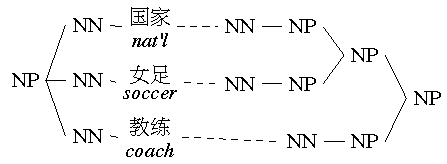
\includegraphics{figures/chinese-tree2} }

\begin{tikzpicture}
\tikzset{every tree node/.style={align=center}}
\Tree
[.NP 
  [.\extranode{NP}
    [.\extranode{NP} [.NN 国家\\national ] ]
    [.\extranode{NP} [.NN 女足\\soccer ] ] ]
  [.\extranode{NP} [.NN 教练\\coach ] ] ]
\end{tikzpicture}

\vspace{3mm}
(a) Parser output

\vspace{6mm}

\begin{tikzpicture}
\tikzset{every tree node/.style={align=center}}
\Tree
[.NP 
  [.NN 国家\\national ]
  [.NN 女足\\soccer ]
  [.NN 教练\\coach ] ]
\end{tikzpicture}

\vspace{3mm}
(b) Gold parse
\derivspace
\caption[Error analysis example: NP internal structure (Chinese).]{ \label{fig:np_internal} 
	\textbf{NP Internal Structure} This should be a flat structure.
}

\end{minipage}\hfill
\begin{minipage}[b]{0.5\textwidth}
\centering
%%%\scalebox{1.2}{ 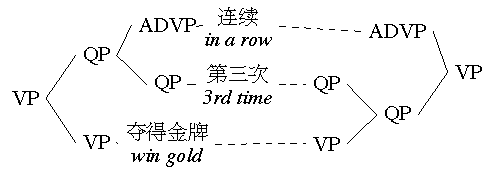
\includegraphics{figures/chinese-treemodatt} }

\begin{tikzpicture}
\tikzset{every tree node/.style={align=center}}
\Tree
[.VP
  [.ADVP 连续\\{in a row} ]
  [.\extranode{QP}
    [.QP 第三次\\{third time} ]
    [.VP 夺得金牌\\{win gold} ] ] ]
\end{tikzpicture}

\vspace{3mm}
(a) Parser output

\vspace{6mm}

\begin{tikzpicture}
\tikzset{every tree node/.style={align=center}}
\Tree
[.VP
  [.\missingnode{QP}
    [.ADVP 连续\\{in a row} ]
    [.QP 第三次\\{third time} ] ]
  [.VP 夺得金牌\\{win gold} ] ]
\end{tikzpicture}

\vspace{3mm}
(b) Gold parse
\derivspace
\caption[Error analysis example: Adverb and adjective modifier attachment (Chinese).]{ \label{fig:mod_att}
  \textbf{Modifier Attachment}: \glos{连续}{in a row} should modify only \glos{第三次}{third time}.
}

\end{minipage}
\end{figure}

\paragraph{NP-internal} (Figure~\ref{fig:np_internal}) \\
The \pctb annotates more NP-internal structure than the \ptb.
We assign this error type when a transformation involves words whose parts of speech in the gold parse are one of: CC, CD, DEG, ETC, JJ, NN, NR, NT and OD.

We investigated the errors that fall into the NP-internal category and found that 49\% of the errors involved the creation or deletion of a single pre-terminal phrasal bracket.
These errors arise when a parser proposes a parse in which POS tags (for instance, JJ or NN) occur as siblings of phrasal tags (such as NP), a configuration used by the PCTB bracketing guidelines to indicate complementation as opposed to adjunction \parencite{Xue:2005:NLE}.

\paragraph{Adverb and Adjective Modifier attachment} (Figure~\ref{fig:mod_att}) \\
Incorrect modifier scope caused by modifier phrase attachment level.
This is less frequent in Chinese than in English: while English VP modifiers occur in pre- and post-verbal positions, Chinese only allows pre-verbal modification.

\paragraph{Wrong sense/bad attachment} (Figure~\ref{fig:sense}) \\
This applies when the head word of a phrase receives the wrong POS, leading to an attachment error.
This error type is common in Chinese because of POS fluidity, \myeg the well-known Chinese verb/noun ambiguity often causes mis-attachments that are classified as this error type.

In Figure~\ref{fig:sense}, the word \mbox{\glos{投资}{invest}} has both noun and
verb senses. While the gold standard interpretation is the relative clause
\mbox{\Trans{firms that Macau invests in}}, the parser returned an NP
interpretation \mbox{\Trans{Macau investment firms}}.

\paragraph{Verb taking wrong args} (Figure~\ref{fig:wrong_arg}) \\
This error type
arises when a verb \mbox{(\myeg~\glos{扭转}{reverse})} is hypothesized to take
an incorrect argument (\mbox{\glos{布什}{Bush}} instead of
\mbox{\glos{地位}{position}}).  Note that this also covers some of the errors
that were classified as NP Attachment for English, changing
the distribution for that type.

\begin{figure}
\begin{minipage}[b]{0.45\textwidth}
\centering
%%%\scalebox{1.2}{ 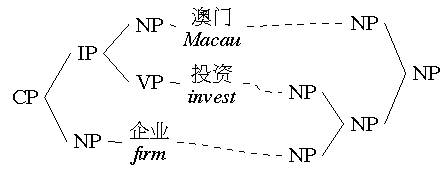
\includegraphics{figures/chinese-tree1} }

\begin{tikzpicture}
\tikzset{every tree node/.style={align=center}}
\Tree
[.\extranode{NP}
  [.NP 澳门\\Macau ]
  [.\extranode{NP}
    [.\extranode{NP} 投资\\invest ]
    [.NP 企业\\firm ] ] ]
\end{tikzpicture}

\vspace{3mm}
(a) Parser output

\vspace{6mm}

\begin{tikzpicture}
\tikzset{every tree node/.style={align=center}}
\Tree
[.\missingnode{CP}
  [.\missingnode{IP}
    [.NP 澳门\\Macau ]
    [.\missingnode{VP} 投资\\invest ] ]
  [.NP 企业\\firm ] ]
\end{tikzpicture}

\vspace{3mm}
(b) Gold parse
\derivspace
\caption[Error analysis example: Word sense confusion (Chinese).]{ \label{fig:sense} 
  \textbf{Sense Confusion} By treating \glos{投资}{invest} as a noun, the parser forms an NP about a type of firm, rather than a clause about action by \Trans{Macau}.
}

\end{minipage}\hfill
\begin{minipage}[b]{0.5\textwidth}
\centering
%%%\scalebox{1.2}{ 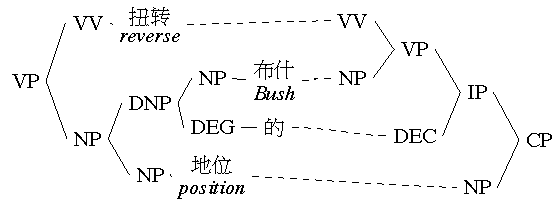
\includegraphics{figures/chinese-treebush} }

\begin{tikzpicture}
\tikzset{every tree node/.style={align=center}}
\Tree
[.\extranode{CP}
  [.\extranode{IP}
    [.\extranode{VP}
      [.VV 扭转\\reverse ]
      [.NP 布什\\Bush ] ]
    [.\extranode{DEC} 的 ] ]
  [.NP 地位\\position ] ]
\end{tikzpicture}

\vspace{3mm}
(a) Parser output

\vspace{6mm}

\begin{tikzpicture}
\tikzset{every tree node/.style={align=center}}
\Tree
[.\missingnode{VP}
  [.VV 扭转\\reverse ]
  [.\missingnode{NP}
    [.\missingnode{DNP}
      [.NP 布什\\Bush ]
      [.\missingnode{DEG} 的 ] ]
    [.NP 地位\\position ] ] ]
\end{tikzpicture}

\vspace{3mm}
(b) Gold parse
\derivspace

\caption[Error analysis example: Verb taking wrong arguments (Chinese).]{ \label{fig:wrong_arg}
  \textbf{Verb Taking Wrong Arguments}: the verb takes the argument \glos{布什}{Bush} too early, before it has been bound with \glos{地位}{position}.
}

\end{minipage}
\end{figure}

\paragraph{Unary} \strut \\
For mis-application of unary rules we separate out instances in which the two brackets in the production have the the same label (A-over-A).
This case is created when traces are eliminated, a standard step in evaluation.
More than a third of unary errors made by the Berkeley parser are of the A-over-A type.
This can be attributed to two factors: (i) the \pctb annotates non-local dependencies using traces, and (ii) Chinese syntax generates more traces than English syntax, such as \emph{pro}-drop, the omission of arguments where the referent is recoverable from discourse \parencite{Guo-Wang-VanGenabith:2007:EMNLP}.
However, for parsers that do not return traces they are a benign error.

\paragraph{Noun boundary error} \strut \\
In this error type, a span is moved to a
position where the POS tags of its new siblings all belong to the
list of NP-internal structure tags which we identified above, reflecting
the inclusion of additional material into an NP.

\paragraph{Split verb compound} \strut \\
The \pctb annotations recognize several
Chinese verb compounding strategies, such as the serial verb construction
(\mbox{\glos{规划建设}{plan [and] build}}) and the resultative construction
(\mbox{\glos{煮熟}{cook [until] done}}), which join a bare verb to another
lexical item.  We introduce an error type specific to Chinese, in which such
verb compounds are split, with the two halves of the compound placed in
different phrases.

\paragraph{Scope error} \strut \\
These are cases in which a new span must be added to more closely bind a modifier phrase (ADVP, ADJP, and PP), for example, in 
(IP (ADVP \mbox{\glos{仅}{Only}}) (NP \mbox{\glos{去年}{last year,}}) (NP \mbox{\glos{中国 银行}{Bank of China}}) \ldots), the ADVP should modify the first NP only, which can be indicated by adding an NP to form (NP (ADVP \mbox{\glos{仅}{Only}}) (NP \mbox{\glos{去年}{last year}})).

\paragraph{PP attachment} \strut \\
This error type is rare in Chinese, as adjunct PPs are pre-verbal.  It does
occur near coordinated VPs, where ambiguity arises about which of the conjuncts
the PP has scope over.  Whether this particular case is PP attachment or
coordination is debatable; we follow the approach above and
label it PP attachment.

\subsection{Chinese-English Comparison} \label{subsec:chinese_english_comparison}

It is difficult to directly compare error analysis results for Chinese and
English parsing because of substantial changes in the classification method,
and differences in treebank annotations.

As described in the previous section, the set of error categories considered for Chinese is very different to the set of categories for English.  
Even for some of the categories that were not substantially changed, errors may be classified differently because of cross-over between two categories (\myeg between Verb taking wrong args and NP Attachment).

Differences in treebank annotations also present a challenge for cross-language error comparison.
The most common error type in Chinese, NP-internal structure, is rare in the English results, but the datasets are not comparable because the \ptb has much more limited NP-internal structure annotated than the \pctb.
Further characterization of the impact of annotation differences on errors is beyond the scope of this work.

Three conclusions that can be made are that (i) coordination is a more common issue in Chinese, but remains difficult in
both languages, (ii) PP attachment is a much greater problem in English, and
(iii) substantial challenges are posed by the higher frequency of
syntactic structures generating traces and null-elements in Chinese compared to English.

\subsection{Cross-Parser Analysis} \label{sec:cross_parser_analysis}

The previous section described the error types and their distribution for a single Chinese parser.
Here we confirm that these are general trends, by showing that the same pattern
is observed for several different parsers on the \pctb 6 dev set.\footnote{
  We use the standard data split suggested by the \pctb 6 file manifest.
  As a result, our results differ from those previously reported on other splits.
}
We include results for
a transition-based parser \parencite[ZPAR;][]{Zhang-Clark:2009:ICPT},
a split-merge PCFG parser \parencite{Petrov-etal:2006,Petrov-Klein:2007,Petrov:2010:NAACLHLT},
a lexicalized parser \parencite{Bikel-Chiang:2000:CLP},
and a factored PCFG and dependency parser
\parencite{Levy-Manning:2003:ACL,Klein-Manning:2003:ACL,Klein-Manning:2003:NIPS}.
\footnote{These parsers represent a variety of parsing methods, though exclude
some recently developed parsers that are not publicly
available \parencite{Qian-Liu:2012:EMNLP,Xiong-etal:2005:IJCNLP}.}

Comparing the two Stanford parsers in Table~\ref{tab:comparison}, the factored
model provides clear improvements on sense disambiguation, but performs
slightly worse on coordination.

The Berkeley product parser we include uses only two grammars because we found,
in contrast to the English results \parencite{Petrov:2010:NAACLHLT}, that further
grammars provided limited benefits.  Comparing the performance with the
standard Berkeley parser it seems that the diversity in the grammars only
assists certain error types, with most of the improvement occurring in four of
the categories, while there is no improvement, or a slight decrease, in five categories.

\begin{landscape}
\begin{table*}
\centering
\setlength\fboxsep{0mm}
\setlength\fboxrule{0.05mm}
\begin{tabular}{|lccccccccccccc|}
	\hline
	    & NP &  & Verb &  & Mod. & 1-Word & Diff & Wrong & Noun & VP & Clause & PP & \\
	System \hfill F$_1$ & Int. & Coord & Args & Unary & Attach & Span & Label & Sense & Edge & Attach & Attach & Attach & Other \\
	\hline
	\hline
	\emph{Best}    & 1.54 & 1.25 & 1.01 & 0.76 & 0.72 & 0.21 & 0.30 & 0.05 & 0.21 & 0.26 & 0.22 & 0.18 & 1.87 \\
	Berk-G$\;$ \hfill 86.8 &  \mybar{3.117775} &  \mybar{5.719997} &  \mybar{4.868075} &  \mybar{4.092204} &  \mybar{3.414187} &  \mybar{1.560478} &  \mybar{2.304226} &  \mybar{0.417061} &  \mybar{3.003337} &  \mybar{4.124765} &  \mybar{4.199998} &  \mybar{3.250795} &  \mybar{3.627305} \\
	Berk-2 \hfill 81.8 &  \mybar{5.106060} &  \mybar{5.726296} &  \mybar{4.657457} &  \mybar{5.602480} &  \mybar{3.889412} &  \mybar{5.874318} &  \mybar{5.465338} &  \mybar{4.259078} &  \mybar{4.180596} &  \mybar{4.645864} &  \mybar{3.974996} &  \mybar{4.055024} &  \mybar{4.120634} \\
	Berk-1 \hfill 81.1 &  \mybar{5.637080} &  \mybar{5.854733} &  \mybar{4.914895} &  \mybar{5.637384} &  \mybar{4.160972} &  \mybar{5.409644} &  \mybar{5.105299} &  \mybar{4.288569} &  \mybar{4.581930} &  \mybar{4.594485} &  \mybar{4.516671} &  \mybar{4.351321} &  \mybar{4.375378} \\
	ZPAR \hfill 78.1 &  \mybar{5.603375} &  \mybar{6.374733} &  \mybar{5.487246} &  \mybar{7.386910} &  \mybar{5.851629} &  \mybar{5.863920} &  \mybar{6.833466} &  \mybar{4.423375} &  \mybar{5.725748} &  \mybar{5.299080} &  \mybar{6.791682} &  \mybar{6.653960} &  \mybar{5.833838} \\
	Bikel \hfill 76.1 &  \mybar{6.464990} &  \mybar{7.357862} &  \mybar{6.227640} &  \mybar{6.372585} &  \mybar{6.280885} &  \mybar{6.602543} &  \mybar{5.609351} &  \mybar{6.904680} &  \mybar{8.000000} &  \mybar{5.790822} &  \mybar{6.700012} &  \mybar{6.484650} &  \mybar{5.983631} \\
	Stan-F \hfill 76.0 &  \mybar{6.824621} &  \mybar{8.000000} &  \mybar{6.340422} &  \mybar{6.721463} &  \mybar{6.291805} &  \mybar{6.949312} &  \mybar{6.977479} &  \mybar{4.827803} &  \mybar{5.886282} &  \mybar{7.060545} &  \mybar{7.166674} &  \mybar{6.933336} &  \mybar{5.501970} \\
	Stan-U \hfill 70.0 &  \mybar{8.000000} &  \mybar{7.035766} &  \mybar{8.000000} &  \mybar{8.000000} &  \mybar{8.000000} &  \mybar{8.000000} &  \mybar{8.000000} &  \mybar{8.000000} &  \mybar{7.464874} &  \mybar{8.000000} &  \mybar{8.000000} &  \mybar{8.000000} &  \mybar{8.000000} \\
	\emph{Worst}   & 3.94 & 1.75 & 1.73 & 1.48 & 1.68 & 1.06 & 1.02 & 0.88 & 0.55 & 0.50 & 0.44 & 0.44 & 4.11 \\
	\hline
\end{tabular}
\caption[Error breakdown for a range of parsers on the \pctb.]{ \label{tab:comparison}
  Error breakdown for the development set of \pctb 6.  The area filled in for
  each bar indicates the average number of bracket errors per sentence attributed
  to that error type, where an empty bar is no errors and a full bar has
  the value indicated in the bottom row.  The parsers are:
  the Berkeley parser with gold POS tags as input (Berk-G),
  the Berkeley parser \parencite[Berk-1;][]{Petrov-etal:2006,Petrov-Klein:2007},
  the Berkeley product parser with two grammars \parencite[Berk-2;][]{Petrov:2010:NAACLHLT},
  ZPAR \textcite{Zhang-Clark:2009:ICPT},
  the Bikel parser \parencite{Bikel-Chiang:2000:CLP},
  the Stanford Factored parser \parencite[Stan-F;][]{Levy-Manning:2003:ACL,Klein-Manning:2003:NIPS},
  and the Stanford Unlexicalized PCFG parser \parencite[Stan-U;][]{Klein-Manning:2003:ACL}.
}
\end{table*}
\end{landscape}

\subsection{Tagging Error Impact} \label{sec:pos_ablation_study}

The challenge of accurate POS tagging in Chinese has been a major part of
several recent papers
\parencite{Qian-Liu:2012:EMNLP,Jiang-etal:2009:ACL,Forst-Fang:2009:EACL}.  The
Berk-G row of Table~\ref{tab:comparison} shows the performance of the Berkeley
parser when given gold POS tags.\footnote{We used the Berkeley parser as it was
the best of the parsers we considered.  Note that the Berkeley parser
occasionally prunes all of the parses that use the gold POS tags,
and so returns the best available alternative.  This leads to a POS accuracy of
99.35\%, which is still well above the parser's standard POS accuracy of
93.66\%.}
While the F$_1$ improvement is unsurprising, for the
first time we can clearly show that the gains are only in a subset of the error
types.  In particular, tagging improvement will not help for two of the most
significant challenges: coordination scope errors, and verb argument
selection.

To see which tagging confusions contribute to which error reductions, we adapt the POS
ablation approach of \textcite{Tse-Curran:2012:NAACL-HLT}.  We consider the POS
tag pairs shown in Table~\ref{tab:pos-confusion}.  To isolate the effects of
each confusion we start from the gold tags and introduce the output of the
Stanford tagger whenever it returns one of the two tags being
considered.\footnote{We introduce errors to gold tags, rather than removing
errors from automatic tags, isolating the effect of a single confusion
by eliminating interaction between tagging decisions.}
We then feed these ``semi-gold'' tags to the
Berkeley parser, and run the fine-grained error analysis on its output.

\begin{table}
  \centering
  \begin{tabular}{|llrr|}
    \hline
      \multicolumn{2}{c}{Confused tags} & Errors & $\Delta$ F$_1$ \\
    \hline
    \hline
      VV  & NN  & 1055 & -2.72 \\
      DEC & DEG &  526 & -1.72 \\
      JJ  & NN  &  297 & -0.57 \\
      NR  & NN  &  320 & -0.05 \\
    \hline
  \end{tabular}
  \caption[The most frequently confused POS tag pairs in Chinese parsing.]{ \label{tab:pos-confusion}
    The most frequently confused POS tag pairs.
    Each $\Delta$ F$_1$ is relative to Berk-G.
  }
\end{table}

\paragraph{VV/NN}  This confusion has been consistently shown to be a major
contributor to parsing errors
\parencite{Levy-Manning:2003:ACL,Tse-Curran:2012:NAACL-HLT,Qian-Liu:2012:EMNLP},
and we find a drop of over 2.7 $F_1$ when the output of the tagger is
introduced.  We found that while most error types have contributions from a
range of POS confusions, verb/noun confusion was responsible for virtually all of
the noun boundary errors corrected by using gold tags.

\paragraph{DEG/DEC}  This confusion between the relativizer and subordinator
senses of the particle \glos{的}{de} is the primary
source of improvements on modifier attachment when using gold tags.

\paragraph{NR/NN and JJ/NN}  Despite their frequency, these confusions have
little effect on parsing performance.  Even within the NP-internal error type
their impact is limited, and almost all of the errors do not change the
logical form.

\section{Summary}

The single F-score objective over brackets or dependencies obscures important differences between statistical parsers.
For instance, one or many mismatched brackets could be caused by a single attachment error.

In Sections~\ref{sec:tree-transform}~and~\ref{sec:classify}, we presented a novel tree-transformation methodology for
evaluating parsers that categorizes errors into linguistically meaningful
types.  Using this approach, we presented the first detailed examination of the
errors produced by a wide range of constituency parsers for
English and Chinese.  We found that PP attachment and clause attachment are the most
challenging constructions in English, while coordination turns out to be less problematic
than previously thought.  We also noted interesting variations in error types
for parser variants.

We investigated the errors resolved in reranking, and introduced by changing
domains. We found that the Charniak rerankers improved most error types, but
made little headway on improving PP attachment.  Changing domain has an impact
on all error types, except NP internal structure.

We also quantified the relative impacts of a comprehensive set of error types
in Chinese parsing.  Our analysis has shown that while improvements in
Chinese POS tagging can make a substantial difference for some error types,
it will not address two high-frequency error types: incorrect verb argument
attachment and coordination scope.  The frequency of these two error types is
also unimproved by the use of products of latent variable grammars.  These
observations suggest that resolving the core challenges of Chinese parsing
will require new developments that suit the distinctive properties of Chinese
syntax.

We released our system so that future constituent parsers could be evaluated using our methodology (see Appendix~\ref{chp:resources}).
Our analysis provides new insight into the development of parsers over the past fifteen years, and the challenges that remain.


\chapter{Formalism Conversion} \label{chp:conversion}

\begin{center}
\textit{
  A preliminary version of this chapter appeared as \textcite{Kummerfeld-etal:2012:ACL}.
}
\end{center}

In this chapter, we propose an improved, bottom-up method for converting \ccg derivations into \ptb-style phrase structure trees.
In contrast with past work \parencite{Clark-Curran:2009}, which used simple rules based on category pairs, our approach follows the generalizations of \ccg, assigning richer rules to individual categories and defining general methods of combining them for each of the \ccg combinators.
Our conversion preserves more sentences under round-trip conversion (51.1\% \myvs 39.6\%) and is more robust.
In particular, unlike past methods, ours does not require ad-hoc rules over non-local features, and so could be integrated into a parser.

\section{Background}

There has been extensive work on converting parser output for evaluation, \myeg
\textcite{Lin:1998} and \textcite{Briscoe-Carroll-Graham-Copestake:2002} proposed
using underlying dependencies for evaluation.  There has also been work on
conversion to phrase structure, from dependencies \parencite{Xia:2001,Xia:2009} and
from lexicalized formalisms, \myeg \hpsg \parencite{Matsuzaki-Tsujii:2008} and \mytag
\parencite{Chiang:2000,Sarkar:2001}. Our focus is on \ccg to \ptb conversion
\parencite{Clark-Curran:2009}.

\subsection{Combinatory Categorial Grammar (\ccg)}

The lower half of Figure~\ref{fig:ccg-example} shows a \ccg derivation
\parencite{Steedman:2000} in which each word is assigned a {\em category}, and
{\em combinatory rules} are applied to adjacent categories until only one
remains.  Categories can be atomic, \myeg the \cf{N} assigned to
\textit{magistrates}, or complex functions of the form {\em result / arg}, where
{\em result} and {\em arg} are categories and the slash indicates the argument's
directionality.  Combinators define how adjacent categories can combine.
Figure~\ref{fig:ccg-example} uses {\em function application}, where a complex
category consumes an adjacent argument to form its result, \myeg \cf{S[dcl]\bs
NP} combines with the \cf{NP} to its left to form an \cf{S[dcl]}.  More
powerful combinators allow categories to combine with greater flexibility.

\begin{figure}
\small
\begin{tikzpicture}[every text node part/.style={align=center}]

  \node (w0) at (0, 0) {\strut Italian \\ \strut $\cf{N/N}$};
  \node (w1) [right=2ex of w0.east] {\strut magistrates \\ \strut $\cf{N}$};
  \node (w2) [right=2ex of w1.east] {\strut labeled \\ \strut $\cf{((S[dcl]\bs NP)/NP)/NP}$};
  \node (w3) [right=2ex of w2.east] {\strut his \\ \strut $\cf{NP[nb]/N}$};
  \node (w4) [right=2ex of w3.east] {\strut death \\ \strut $\cf{N}$};
  \node (w5) [right=2ex of w4.east] {\strut a \\ \strut $\cf{NP[nb]/N}$};
  \node (w6) [right=2ex of w5.east] {\strut suicide \\ \strut $\cf{N}$};

% PTB above
  \node (nt03) [above=3ex of w3.north] {PRP\$};
  \node (nt04) [above=3ex of w4.north] {NN};
  \node (nt05) [above=3ex of w5.north] {DT};
  \node (nt06) [above=3ex of w6.north] {NN};
  \path (nt03.north) -- node[above=3ex] (nt13-14) {NP} (nt04.north);
  \path (nt05.north) -- node[above=3ex] (nt15-16) {NP} (nt06.north);
  \path (nt13-14.north) -- node[above=3ex] (nt23-26) {S} (nt15-16.north);
  \node (nt20) at (w0 |- nt23-26) {JJ};
  \node (nt21) at (w1 |- nt23-26) {NNS};
  \node (nt22) at (w2 |- nt23-26) {VBD};
  \path (nt20.north) -- node[above=3ex] (nt30-31) {NP} (nt21.north);
  \path (nt22.north) -- node[above=3ex] (nt32-36) {VP} (nt23-26.north);
  \path (nt30-31.north) -- node[above=3ex] (nt40-46) {S} (nt32-36.north);

  \draw (w0.north) -- (nt20.south);
  \draw (w1.north) -- (nt21.south);
  \draw (w2.north) -- (nt22.south);
  \draw (w3.north) -- (nt03.south);
  \draw (w4.north) -- (nt04.south);
  \draw (w5.north) -- (nt05.south);
  \draw (w6.north) -- (nt06.south);
  \draw (nt03.north) -- (nt13-14.south) -- (nt04.north);
  \draw (nt05.north) -- (nt15-16.south) -- (nt06.north);
  \draw (nt13-14.north) -- (nt23-26.south) -- (nt15-16.north);
  \draw (nt20.north) -- (nt30-31.south) -- (nt21.north);
  \draw (nt22.north) -- (nt32-36.south) -- (nt23-26.north);
  \draw (nt30-31.north) -- (nt40-46.south) -- (nt32-36.north);

% CCG below
  \node (c00L) at (w0.south west) {};
  \node (c00R) at (w1.south east) {};
  \draw [-{Straight Barb[length=2mm]}] (c00L) -- node[below=0ex] (c00) {\strut $\cf{N}$} (c00R);
  \node (c01L) at (w3.south west) {};
  \node (c01R) at (w4.south east) {};
  \draw [-{Straight Barb[length=2mm]}] (c01L) -- node[below=0ex] (c01) {\strut $\cf{NP[nb]}$} (c01R);
  \node (c02L) at (w5.south west) {};
  \node (c02R) at (w6.south east) {};
  \draw [-{Straight Barb[length=2mm]}] (c02L) -- node[below=0ex] (c02) {\strut $\cf{NP[nb]}$} (c02R);
  \node (c10L) at (c00L |- c00.south) {};
  \node (c10R) at (c00R |- c00.south) {};
  \draw (c10L) -- node[below=0ex] (c10) {\strut $\cf{NP}$} (c10R);
  \node (c11L) at (w2.west |- c01.south) {};
  \node (c11R) at (w4.east |- c01.south) {};
  \draw [-{Straight Barb[length=2mm]}] (c11L) -- node[below=0ex] (c11) {\strut $\cf{(S[dcl]\bs NP)/NP}$} (c11R);
  \node (c20L) at (w2.west |- c11.south) {};
  \node (c20R) at (w6.east |- c11.south) {};
  \draw [-{Straight Barb[length=2mm]}] (c20L) -- node[below=0ex] (c20) {\strut $\cf{S[dcl]\bs NP}$} (c20R);
  \node (c30L) at (w0.west |- c20.south) {};
  \node (c30R) at (w6.east |- c20.south) {};
  \draw [-{Straight Barb[reversed,length=2mm]}] (c30L) -- node[below=0ex] (c30) {\strut $\cf{S[dcl]}$} (c30R);
\end{tikzpicture}

\caption[An example of \ccg and \ptb parses with nodes covering crossing spans.]{ \label{fig:ccg-example}
  An example of \ccg and \ptb parses with nodes covering crossing spans: \emph{his death a suicide} (\ptb) and \emph{labeled his death} (CCGbank).
}
\end{figure}

We cannot form a \ptb tree by simply relabeling the categories in a \ccg derivation for two reasons.
First, the mapping from categories to phrase labels is many-to-many, so it would be difficult to determine the correct label (though other researchers have tried, as discussed in Section~\ref{sec-learned-conv}).
Second, there are some spans that occur only in the \ccg derivation and others that occur only in the \ptb parse, \myeg in Figure~\ref{fig:ccg-example} there is a node for \emph{his death a suicide} in \ptb but not \ccg, and vice versa for \emph{labeled his death} (CCGbank).
This second issue is particularly difficult because in some cases, including the example given, the differing nodes in the two parses cover spans of the sentence that cross\footnote{This means a local insertion or deletion of a node cannot make the necessary changes, there would have to be several simultaneous changes to go from one structure to the other.}.
These differences are the result of conscious decisions made in the construction of CCGbank, in many cases enabling the derivation to encode extra dependencies that are either implicit or expressed via traces in the \ptb.

\subsection{\textcite{Clark-Curran:2009}}

\begin{table}[t!]
\centering
\begin{tabular}{l|l}
\hline
Categories & Schema \\
\hline\hline
\cf{N} & create an NP \\
\cf{((S[dcl]\bs NP)/NP)/NP} & create a VP \\
\hline
\cf{N/N} + \cf{N} & place left under right \\
\cf{NP[nb]/N} + \cf{N} & place left under right \\
\cf{((S[dcl]\bs NP)/NP)/NP} + \cf{NP} & place right under left \\
\cf{(S[dcl]\bs NP)/NP} + \cf{NP} & place right under left \\
\cf{NP} + \cf{S[dcl]\bs NP} & place both under S\\
\hline
\end{tabular}
\caption[Example rules from \textcite{Clark-Curran:2009}.]{ \label{fig:candc09}
  Example \old lexical and rule schemas.
}
\end{table}

\textcite{Clark-Curran:2009}, hereafter \old, assign a {\em schema} to each
leaf (lexical category) and rule (pair of combining categories) in the \ccg derivation.
The \ptb tree is constructed from the \ccg bottom-up, creating leaves with
lexical schemas, then merging/adding sub-trees using rule schemas at each step.

The schemas for Figure~\ref{fig:ccg-example} are shown in Table~\ref{fig:candc09}.
These apply to create NPs over \textit{magistrates}, \textit{death}, and
\textit{suicide}, and a VP over \textit{labeled}, and then combine the trees by
placing one under the other at each step, and finally create an S node at the
root.

\old has sparsity problems, requiring schemas for all valid pairs of
categories --- at a minimum, the 2853 unique category combinations found in
CCGbank. \textcite{Clark-Curran:2009} create schemas for only 776 of these,
handling the remainder with approximate catch-all rules.

\old only specifies one simple schema for each rule (pair of
categories).  This appears reasonable at first, but frequently causes
problems, \myeg:

\begin{center}
\cf{(N/N)/(N/N)} + \cf{N/N} \\
\begin{tabular}{ll}
  (1) & ``more than'' + ``30'' \\ % should form a QP
  (2) & ``relatively'' + ``small'' \\ % should from an ADJP
\end{tabular}
%%%% ((N/N)/(N/N))\(S[adj]\NP) IN than
%%%% (N/N)/(N/N) RB relatively
\end{center}

Here either a QP bracket (1) or an ADJP bracket (2) should be created.  Since
both examples involve the same rule schema, \old would incorrectly process them
in the same way.  To combat the most glaring errors, \old manipulates the \ptb
tree with ad-hoc rules based on non-local features over the \ccg nodes
being combined --- an approach that cannot be easily integrated into a
parser.

These disadvantages are a consequence of failing to exploit the generalizations that \ccg combinators define. 
We return to this example below to show how our approach does exploit those generalizations and thereby handles both cases correctly.

\subsection{\textcite{zhang-zhao-hui:2012:DEMOS}} \label{sec-learned-conv}

\textcite{zhang-zhao-hui:2012:DEMOS} considered a statistical approach to conversion from \ccg to \ptb.
Their system works by classifying each step in the \ccg derivation as either being a \ptb node or being a dummy node, to be flattened in the final structure.
This approach has the limitation that it cannot handle sentences where the structure of the \ccg derivation is missing nodes that exist in the structure of the \ptb parse, such as the example in Figure~\ref{fig:ccg-example}.
These cases account for 10\% of sentences, but the method is still fairly effective because they are able to recover most of the structure for such sentences.

\section{Our Approach}

\begin{figure}
\centering
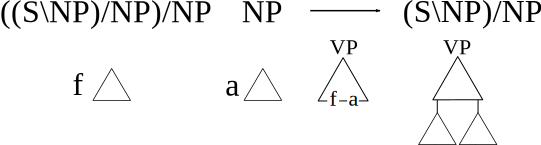
\includegraphics[width=0.85\linewidth]{figures/ccg-example}
\caption[An example function application during \ccg to \ptb conversion.]{ \label{fig:inst-example}
  An example function application.
  Top row: \ccg rule.
  Bottom row: applying instruction (VP f a).
}
\end{figure}

\begin{table}
\centering
\begin{tabular}{lll}
	\hline
		Symbol & Meaning & Example Instruction \\
	\hline
	\hline
		(X f a) & Add an X bracket around functor and argument & (VP$\;$ f$\;$ a) \\
		\{ \} & Flatten enclosed node & (N$\;$ f$\;$ \{a\}) \\
		X* & Use same label as argument or default to X & (S*$\;$ f$\;$ \{a\}) \\
		f$_i$ & Place subtrees &  (PP$\;$ f$_0$$\;$ (S$\;$ f$_{1..k}$$\;$ a)) \\
	\hline
\end{tabular}
\caption[Types of operations in instructions in our \ccg to \ptb conversion.]{\label{tab:operators}
  Types of operations in instructions.
}
\end{table}

Our conversion assigns a set of instructions to each lexical category and defines generic operations for each combinator that combine instructions.
Figure~\ref{fig:inst-example} shows an example of a common form of instruction \emph{(VP f a)}, which specifies three things:

\begin{itemize}
  \item Create a new VP node, indicated by the VP and brackets
  \item Place the \ptb parse for the functor under the new node, on the left, indicated by the position of the f
  \item Place the \ptb parse for the argument under the new node, on the right, indicated by the position of the a
\end{itemize}

Table~\ref{tab:operators} shows all of the operators we define.
For convenience, in this description we will refer to the parses coming from the functor and argument as sub-parses.
The first operator is the one described above, though note that it can be more powerful, constructing any set of \ptb nodes indicated with standard bracket notation plus the two markers for the functor and argument.
The \{~\} operator indicates that a flattened version of that sub-parse should be placed, in the example in the table the top node in the sub-parse for the argument would be deleted so its children are placed instead.
The * operator takes the label for the new node from the argument sub-parse, \myeg the result of an \cf{S\bs S_1} should correspond to the label of argument 1 (SINV, SBAR, etc, which all appear as \cf{S} in \ccg).
This is necessary because CCGBank uses additional annotations on categories to distinguish cases that are assigned entirely different labels in the \ptb.
The final operator enables breaking up children in a sub-parse and placing them at different locations in the structure being formed.
This only makes sense when creating multiple nodes, a PP and an S in the example, and uses subscripts to indicate which sub-parse to place where.
Finally, complex categories with multiple arguments are assigned a list of instructions, one per argument.

The lists of rules are processed by following the \ccg derivation, taking actions depending on the type of combinator used:

\vspace{5mm}
\noindent
\textbf{Lexical assignment:} The initial instruction list for a category is taken from our hand-annotated set.

\vspace{3mm}
\noindent
\begin{minipage}[c]{0.6\textwidth}
\textbf{Function application:} The next rule in the functor's list is applied and any remaining rules in its list are retained as the new rule set (any rules remaining in the list for the argument are discarded).
\end{minipage}\hfill
\begin{minipage}[c]{0.3\textwidth}
\zerodisplayskips
\begin{align*}
  \cf{X / Y} \quad & \quad \cf{Y}       & \Rightarrow & \quad \cf{X} \\
  \cf{Y}     \quad & \quad \cf{X \bs Y} & \Rightarrow & \quad \cf{X}
\end{align*}
\end{minipage}

\vspace{3mm}
\noindent
\begin{minipage}[c]{0.6\textwidth}
\textbf{Function composition:} The unapplied instructions of the argument are inserted into the remaining steps for the functor.
\end{minipage}\hfill
\begin{minipage}[c]{0.3\textwidth}
\zerodisplayskips
\begin{align*}
  \cf{X / Y} \quad   & \quad \cf{Y / Z}   & \Rightarrow & \quad \cf{X / Z} \\
  \cf{Y \bs Z} \quad & \quad \cf{X \bs Y} & \Rightarrow & \quad \cf{X \bs Z}
\end{align*}
\end{minipage}

\vspace{3mm}
\noindent
\begin{minipage}[c]{0.6\textwidth}
\textbf{Crossed composition:}
Only backwards crossed composition is used (the lower of the two).
The new instruction list is composed of the top rule from the left, followed by all but the top rule from the right.
\end{minipage}\hfill
\begin{minipage}[c]{0.3\textwidth}
\zerodisplayskips
\begin{align*}
  \cf{X / Y} \quad & \quad \cf{Y \bs Z} & \Rightarrow & \quad \cf{X \bs Z} \\
  \cf{Y / Z} \quad & \quad \cf{X \bs Y} & \Rightarrow & \quad \cf{X / Z}
\end{align*}
\end{minipage}

\vspace{3mm}
\noindent
\begin{minipage}[c]{0.6\textwidth}
\textbf{Type raising:}
A new list of instructions is taken from our hand-annotated set.
If necessary, the current structure is flattened to prevent a unary production of identical symbols being formed when the next instruction is applied.
\end{minipage}\hfill
\begin{minipage}[c]{0.3\textwidth}
\zerodisplayskips
\begin{align*}
  \cf{Y} & \Rightarrow & \quad \cf{T / (T \bs X)} \\
  \cf{X} & \Rightarrow & \quad \cf{T \bs (T / X)}
\end{align*}
\end{minipage}

\vspace{3mm}
\noindent
\textbf{Coordination:}
In \ccg coordination is a single step, but for implementation in parsing it is typically broken into two steps.
We follow the derivation, doing the core structural construction in the second step.
The instructions retained after the second step are from the right conjunct.

\vspace{3mm}
\noindent
\textbf{Functional substitution:}
These combinators occur rarely in the treebank and are not used in current parsers, so we do not implement them.
\vspace{5mm}

Additionally, we vary the instructions assigned based on the \pos tag in 32 cases, and for the word \textit{not}, to recover distinctions not captured by CCGbank categories alone.
In 52 cases the later instructions depend on the structure of the argument being picked up, often to capture different handling of adverbial and adjectival phrases.
For the non-combinatory binary and unary rules in CCGbank we define twenty-eight special instruction sets.

\begin{table}
\centering
\begin{tabular}{lll}
	\hline
		Category & Instruction set \\
	\hline
	\hline
		\cf{N} & (NP$\;$ f) \\[1pt]
		\cf{N/N_1} & (NP$\;$ f$\;$ \{a\}) \\[1pt]
		\cf{NP[nb]/N_1} & (NP$\;$ f$\;$ \{a\}) \\[1pt]
		\cf{((S[dcl]\bs NP_3)/NP_2)/NP_1} & (VP$\;$ f$\;$ a) \\
		 & (VP$\;$ \{f\}$\;$ a) \\
		 & (S$\;$ a$\;$ f) \\
	\hline
\end{tabular}
\caption[Example instructions for our \ccg to \ptb conversion.]{ \label{tab:instructions}
  Instruction sets for the categories in Figure~\ref{fig:ccg-example}.
}
\end{table}

For the example from the previous section we begin by assigning the instructions shown in Table~\ref{tab:instructions}.
Some of these can apply immediately as they do not involve an argument, \myeg \textit{magistrates} has (NP$\;$~f), producing:

\begin{center}
\scalebox{\inlinederivscale}{
\synttree
[NP
	[NNS [magistrates]]]
}
\end{center}

A slightly more complicated instruction is applied to \textit{Italian}: (NP~f~\{a\}).
This creates a new NP bracket, inserts the functor's tree, and flattens and inserts the argument's tree, producing:

\begin{center}
\scalebox{\inlinederivscale}{
\synttree
[NP
	[JJ [Italian]]
	[NNS [magistrates]]]
}
\end{center}

Similar operations apply for the other NPs, followed by a unary rule, mapping \cf{N} to \cf{NP}.
We handle this by applying one of the special cases for non-combinatory unary operations in CCGbank.

The next three steps all involve instructions from the verb's list.
The verb takes three arguments, and so has three instructions applied as follows:

\begin{center}
\strut
\hfill
\scalebox{\inlinederivscale}{
\synttree
[VP
  [VBD [labeled]]
  [NP
	  [PRP\$ [his]]
	  [NN [death]]]]
}
\hfill
\scalebox{\inlinederivscale}{
\synttree
[VP
  [VBD [labeled]]
  [NP
	  [PRP\$ [his]]
	  [NN [death]]]
  [NP
	  [DT [a]]
	  [NN [suicide]]]]
}
\hfill
\strut
\\
\strut
\hfill
\scalebox{\inlinederivscale}{
\synttree
[S
  [NP
    [JJ [Italian]]
    [NNS [magistrates]]]
  [VP
    [VBD [labeled]]
    [NP
      [PRP\$ [his]]
      [NN [death]]]
    [NP
      [DT [a]]
      [NN [suicide]]]]]
}
\hfill
\strut
\end{center}

The final tree in this case is almost correct but omits the S bracket around the two NPs on the right.
To fix it we could have modified \textit{labeled}'s second instruction to move \textit{his death} under a new S via the final symbol in Table~\ref{tab:operators}.
However, for this particular construction the \ptb annotations are inconsistent, and so we cannot recover without introducing more errors elsewhere.

Our approach naturally handles our QP \myvs ADJP example from the previous section because the two cases have different lexical categories: 

\begin{center}
{\small\cf{((N/N)/(N/N))\bs (S[adj]\bs NP)}} on \textit{than} and \\
{\small \cf{(N/N)/(N/N)}} on \textit{relatively}
\end{center}

This lexical difference means we can assign different instructions to correctly recover the QP and ADJP nodes, whereas \old applies the same schema in both cases because after the first function application for \textit{than}, the category becomes the same as the category for \textit{relatively}.

\section{Evaluation}

Using sections 00-21 of the treebanks, we hand-crafted instructions for 527 lexical categories, a process that took under 100 hours, and includes all the categories used by the \candc parser.
There are 647 further categories and 35 non-combinatory binary rules in sections 00-21 that we did not annotate.
For unannotated categories, we use the instructions of the result category with an added instruction.

\begin{table}
\centering
\begin{tabular}{lc@{\hskip 7.5mm}cccc@{\hskip 7.5mm}cccc}
  \hline
           &      & \multicolumn{4}{c}{Length $\le 40$} & \multicolumn{4}{c}{All lengths} \\
    System & Data & P & R & F & Sent. & P & R & F & Sent. \\
  \hline
  \hline
    \multirow{2}{*}{\old}
           & 00  & 94.39 & 95.85 & 95.12 & 42.1 & 93.67 & 95.37 & 94.51 & 39.6 \\
           & 23  & 94.04 & 95.44 & 94.73 & 41.9 & 93.95 & 95.33 & 94.64 & 39.7 \\
  \hline
    \multirow{2}{*}{Zhang, et al. (2012)}
           & 00  & 97.09 & 95.40 & 96.24 & --   & 96.92 & 94.82 & 95.86 & -- \\
           & 23  & 96.69 & 94.79 & 95.73 & --   & 96.67 & 94.77 & 95.71 & -- \\
  \hline
    \multirow{2}{*}{This work}
           & 00  & 96.98 & 96.77 & 96.87 & 53.6 & 96.69 & 96.58 & 96.63 & 51.1 \\
           & 23  & 96.57 & 96.21 & 96.39 & 53.8 & 96.49 & 96.11 & 96.30 & 51.4 \\
  \hline
\end{tabular}
\caption{\label{tab:conversion-comparison}
	\parseval Precision, Recall, F-Score, and exact sentence match for converted
	gold \ccg derivations.
}
\end{table}

Table~\ref{tab:conversion-comparison} compares our approach with \old and \textcite{zhang-zhao-hui:2012:DEMOS} on gold \ccg derivations.
The results shown are as reported by \evalb \parencite{Black-etal:1991} using the \textcite{Collins:1997} parameters.
Our approach leads to increases over \old on all metrics of at least 1.1\%, and increases exact sentence match by over 11\% (both absolute).

Many of the remaining errors relate to missing and extra clause nodes and a range of rare structures, such as QPs, NACs, and NXs.
The only other prominent errors are single word spans, \myeg extra or missing ADVPs.
Many of these errors are unrecoverable from CCGbank, either because inconsistencies in the \ptb have been smoothed over or because they are genuine but rare constructions that were lost.

\begin{figure}
\centering
  \hfill
  \scalebox{0.85}{ 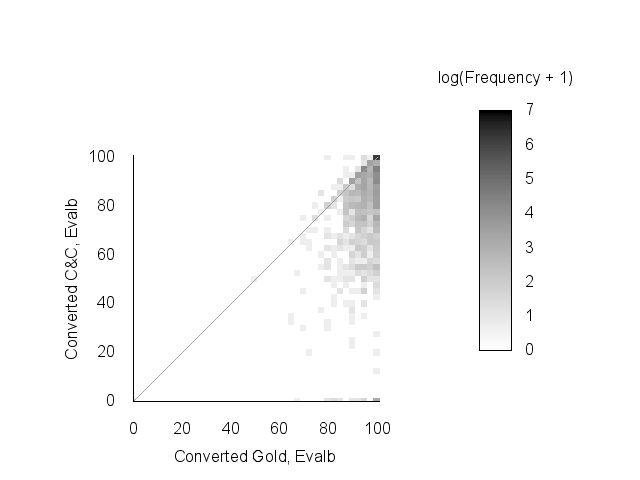
\includegraphics[trim={110mm 25mm 10mm 15mm},clip]{figures/heat-converted} }
  \hfill
  \scalebox{0.85}{ 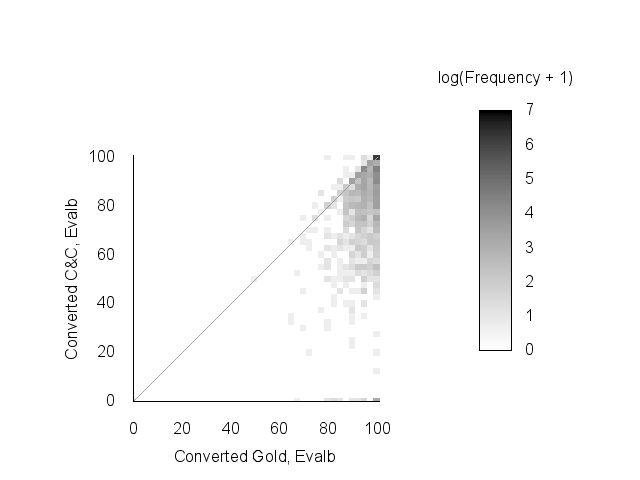
\includegraphics[trim={15mm 0 55mm 40mm},clip]{figures/heat-converted} }
	\\
  \scalebox{0.85}{ 
    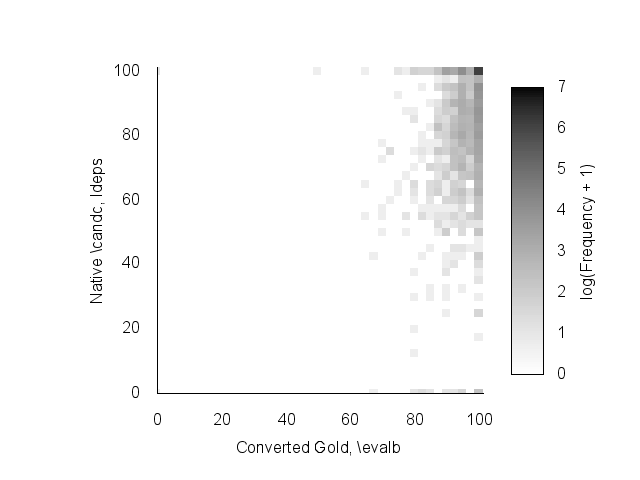
\includegraphics[trim={15mm 0 50mm 40mm},clip]{figures/heat-native}
    \hfill
    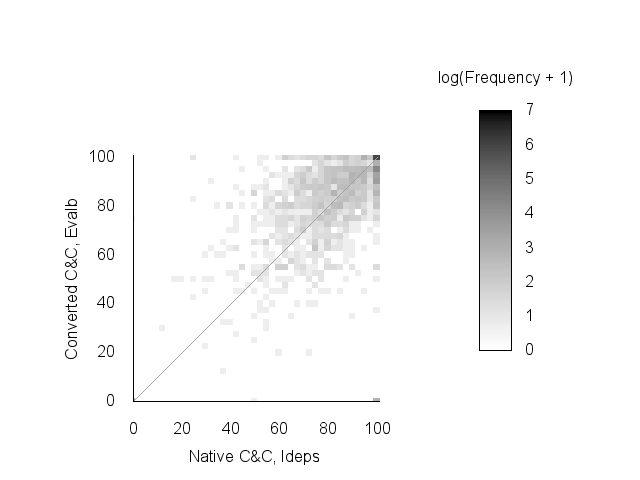
\includegraphics[trim={15mm 0 65mm 40mm},clip]{figures/heat-both}
  }
	\caption[Heatmaps comparing gold conversion accuracy, \ccg native evaluation, and converted evaluation.]{ \label{fig:scatter_plots}
		For each sentence in the treebank, we plot the converted parser output against gold conversion (top), the original parser evaluation against gold conversion (left), and the converted parser output against the original parser evaluation against (right).
		A diagonal line indicating $x=y$ is also included.
		Top: Most points lie below the diagonal, indicating that the quality of converted parser output (y) is upper bounded by the quality of conversion on gold parses (x).
		Left: No clear correlation is present, indicating that the set of sentences that are converted best (on the far right), are not necessarily easy to parse.
		Right: In general, accuracy on the native metric is correlated with accuracy after conversion.
	}
\end{figure}

\subsection{Parser Comparison}

When we convert the output of a \ccg parser, the \ptb trees that are produced
will contain errors created by our conversion as well as by the parser. In this
section we are interested in comparing parsers, so we need to factor out errors
created by our conversion.

One way to do this is to calculate a projected score (Proj), as the
parser result over the oracle result, but this is a very rough approximation.
Another way is to evaluate only on the 51\% of sentences for which our
conversion from gold \ccg derivations is perfect (Clean).  However,
even on this set our conversion introduces errors, as when the parser output differs from the gold derivation, it may
contain categories that are harder to convert.

Parser F-scores are generally higher on Clean, which could mean that this
set is easier to parse, or it could mean that these sentences don't contain
annotation inconsistencies, and so the parsers aren't incorrect for returning
the true parse (as opposed to the one in the \ptb).  To test this distinction
we look for correlation between conversion quality and parse difficulty on
another metric.  In particular, Figure~\ref{fig:scatter_plots} (bottom left) shows
\ccg labeled dependency performance for the \candc parser \myvs CCGbank
conversion \parseval scores. The lack of a strong correlation, and the spread
on the line $x=100$, supports the theory that these sentences are not
necessarily easier to parse, but rather have fewer annotation inconsistencies.

In the top plot, the y-axis is \parseval on converted \candc parser output.
Conversion quality essentially bounds the performance of the parser.
The few points above the diagonal are mostly short sentences on which the \candc parser uses categories that lead to one extra correct node (a common case is ADVP v ADJP).
The main constructions on which parse errors occur, \myeg PP attachment, are rarely converted incorrectly, and so we expect the number of errors to be cumulative.
The bottom right plot shows three noteworthy properties, (1) in general the two evaluation metrics are correlated, (2) the \ccg evaluation is slightly harsher, with fewer points below the diagonal line than above it\footnote{This is consistent with prior work, and the fact that \ccg makes some additional distinctions, such as between arguments and adjuncts.}, (3) there are some very common cases on the far right, where the \ccg evaluation is perfect, but conversion mistakes mean the \ptb score is not perfect.
Some sentences are higher in the right plot than the left because there are distinctions in \ccg that are not always present in the \ptb, \myeg the argument-adjunct distinction.

\begin{table}
\centering
\begin{tabular}{lrr|r}
	\hline
	Sentences & Clean & All & Proj \\
	\hline
	\hline
		\multicolumn{2}{l}{Converted gold \ccg} & & \\
		CCGbank & \hspace{0mm}100.0 & \hspace{0mm}96.3 & -- \\
	\hline
		\multicolumn{2}{l}{Converted \ccg} & & \\
		\textcite{Clark-Curran:2007} & 90.9 & 85.5 & 88.8 \\
		\textcite{Fowler-Penn:2010} & 90.9 & 86.0 & 89.3 \\
		\textcite{Auli-Lopez:2011} & 91.7 & 86.2 & 89.5 \\
	\hline
		\multicolumn{2}{l}{Native \ptb} & & \\
		\textcite{Klein-Manning:2003:ACL} & 89.8 & 85.8 & -- \\
		\textcite{Petrov-Klein:2007} & 93.6 & 90.1 & -- \\
		\textcite{Charniak-Johnson:2005} & 94.8 & 91.5 & -- \\
	\hline
\end{tabular}
\caption[F-scores on section 23 for \ptb parsers and \ccg parsers with their output converted by our method.]{ \label{tab:full-comp}
	F-scores on section 23 for \ptb parsers and \ccg parsers with their output converted by our method.
	Clean is only on sentences that are converted perfectly from gold \ccg (51\%).
	All is over all sentences.
	Proj is a projected F-score (All result / CCGbank All result).
}
\end{table}

Table~\ref{tab:full-comp} presents F-scores for three \ptb parsers and three
\ccg parsers (with their output converted by our method).  One interesting
comparison is between the \ptb parser of \textcite{Petrov-Klein:2007} and the
\ccg parser of \textcite{Fowler-Penn:2010}, which use the same underlying
parser.  The performance gap is partly due to structures in the \ptb that are
not recoverable from CCGbank, but probably also indicates that the split-merge
model is less effective in \ccg, which has far more symbols than the \ptb.

It is difficult to make conclusive claims about the performance of the parsers.
As shown earlier, Clean does not completely factor out the errors
introduced by our conversion, as the parser output may be more difficult to
convert, and the calculation of Proj only roughly factors out the
errors.  However, the results do suggest that the performance of the \ccg
parsers is somewhere between the Stanford and Petrov parsers.

\section{Summary}

By exploiting the generalized combinators of the \ccg formalism, we developed a new method of converting \ccg derivations into \ptb-style trees.
Our system is more effective than previous work, increasing exact sentence match by more than 11\% (absolute), and can be directly integrated with a \ccg parser.
The system is available online, see Appendix~\ref{chp:resources}.


\chapter{Graph Parsing}

\section{Algorithm}

\tikzset{% 
  not allowed/.style={%
    dotted,
    very thick,
    color=red
  }
}
\tikzset{% 
  required/.style={%
  }
}
\tikzset{% 
  optional/.style={%
    dashed
  }
}
\tikzset{% 
  pointO/.style={%
    fill=black,regular polygon, regular polygon sides=4,inner sep=1pt
  }
}
\newlength\vertSmall
\newlength\vertBig
\newlength\vertBigger
\newlength\labelGap
\newlength\coordGap

\newenvironment{tightflushright}{
  \null\hfill
}{
}

\subsection{Parsing Algorithm for Graphs}

% TODO - Add the intuition that when edges are added to/from the external point
% to the span, those edges are all going to be crossed at some point in the
% future.

In this section we sketch our algorithm, focusing on how it differs from \textcite{ec}'s tree parsing algorithm.
For the full derivation see the supplementary material.

The algorithm is a dynamic program defined by (1) a set of items, and (2) deduction rules that define how an item can be composed from other items.
To make the deduction rules manageable, we define some constraints explicitly, and then use code to enumerate all options and enforces additional constraints.
The representation described above requires directed, labeled edges, and spines.
To simplify the presentation of the algorithm we first focus on deduction rules for undirected, unlabeled edges and ignore spines, then return to these later.

To enable efficient parsing we restrict the space we consider, not covering a few specific one-endpoint-crossing structures as described earlier.
In practice, these structures are rarely observed in the PTB, and when they do occur it is usually due to where punctuation attaches.

\paragraph{Notation}
We use $p$, $q$, etc to refer to word positions.
To indicate ranges we use $[pq]$, $[pq)$, $(pq]$, or $(pq)$, where the bracket variations indicate inclusion, $[]$, or exclusion, $()$, of the endpoint.
To indicate an edge we use two points without brackets, \myeg $pq$.
To define a class of edges we either use a point and a set connected by a dash, \myeg $o$--$(pq)$, or two sets connected by a dash, \myeg $(ps)$--$(sq)$.

\subsubsection{Item Types}

Rather than the conventional constituency parsing approach where items fully cover words and end in the gaps between words, our items fully cover the gaps and end on the words, as shown in Figure~\ref{fig:alg-example}, and like in \textcite{eisner-satta-1999}'s algorithm.
We use six item types, differing in the type of edge crossing they contain.  \\

\hspace{-8mm}
\begin{tabular}{l@{\hskip 3pt}l}
  \begin{tikzpicture}
    \node (p) at (0.5, 0) {$p$};
    \node (q) at (1.5, 0) {$q$};
    \draw (p.north) -- (q.north);
  \end{tikzpicture} &
  \parbox{0.36\textwidth}{
    \textbf{$I$, Interval}
    A span in which all points in $(pq)$ have a parent in $[pq]$, and no edges exist that go from outside $[pq]$ to points in $(pq)$. \\
  } \\
  \begin{tikzpicture}
    \node (p) at (0, 0) {};
    \node (q) at (1, 0) {};
    \node (o) at (1.5, 0) {$o$};
    \draw (p.north) -- (q.north);
    \draw [out=45,in=135] (p.north) to (o.north);
  \end{tikzpicture} &
  \parbox{0.36\textwidth}{
    \textbf{$X$, Exterval}
    An interval plus a single edge between $o$ and either $p$ or $q$, where $o$ is outside $[pq]$. \\
  } \\
  \begin{tikzpicture}
    \node (p) at (0, 0) {};
    \node (m1) at (0.2, 0) {};
    \node (m2) at (0.4, 0) {};
    \node (m3) at (0.6, 0) {};
    \node (m4) at (0.8, 0) {};
    \node (q) at (1, 0) {};
    \node (o) at (1.5, 0) {};
    \draw (p.center) -- (q.center);
    \draw [out=45,in=135] (m1.center) to (o.center);
    \draw [out=45,in=135] (m4.center) to (o.center);
    \draw [out=45,in=135] (p.center) to (m2.center);
    \draw [out=45,in=135] (m3.center) to (q.center);
  \end{tikzpicture} &
  \parbox{0.36\textwidth}{
    \textbf{$B$, Both}
    An interval $[pq]$ and a point $o$.
    $o$--$(pq)$ edge may be crossed by $p$--$(pq)$ or $q$--$(pq)$ edges, and at least one crossing of each type occurs. \\
  } \\
  \begin{tikzpicture}
    \node (p) at (0, 0) {};
    \node (m) at (0.3, 0) {};
    \node (m2) at (0.6, 0) {};
    \node (q) at (1, 0) {};
    \node (o) at (1.5, 0) {};
    \draw (p.center) -- (q.center);
    \draw [out=45,in=135] (m.center) to (o.center);
    \draw [out=45,in=135] (p.center) to (m2.center);
  \end{tikzpicture} &
  \parbox{0.36\textwidth}{
    \textbf{$L$, Left}
    Same as $B$, but $o$--$(pq)$ edges may only be crossed by $p$--$(pq)$ edges. \\
  } \\
  \begin{tikzpicture}
    \node (p) at (0, 0) {};
    \node (m) at (0.3, 0) {};
    \node (m2) at (0.6, 0) {};
    \node (q) at (1, 0) {};
    \node (o) at (1.5, 0) {};
    \draw (p.center) -- (q.center);
    \draw [out=45,in=135] (m2.center) to (o.center);
    \draw [out=45,in=135] (m.center) to (q.center);
  \end{tikzpicture} &
  \parbox{0.36\textwidth}{
    \textbf{$R$, Right}
    Same as $L$, but with edges crossed by $q$--$(pq)$ edges rather than $p$-$(pq)$ edges. \\
  } \\
  \begin{tikzpicture}
    \node (p) at (0, 0) {};
    \node (m) at (0.5, 0) {};
    \node (q) at (1, 0) {};
    \node (o) at (1.5, 0) {};
    \draw (p.center) -- (q.center);
    \draw [out=45,in=135] (m.center) to (o.center);
  \end{tikzpicture} &
  \parbox{0.36\textwidth}{
    \textbf{$N$, Neither}
    An interval and a point, with a least one $o$--$(pq)$ edge.
    $o$--$(pq)$ edges can only be crossed by $pq$, not other $[pq]$--$[pq]$ edges. \\
  }
\end{tabular}

Comparing these definitions with the items in \textcite{ec}, we have one entirely new type, the Exterval, and we have added the requirement that the later items have at least one crossing of the specified type.
These changes are necessary to avoid derivational ambiguity when a structure falls into multiple classes.
Enforcing these difference involves changes throughout the deduction rules.

\subsubsection{Example Derivation}

\begin{figure}
\centering

\tikzset{% 
  leftChild/.style={%
    ->,
    >=Stealth,
    shorten >=1pt,
    thin
  }
}

\tikzset{% 
  rightChild/.style={%
    <-,
    >=Stealth,
    shorten <=1pt,
    thin
  }
}

\tikzset{% 
  len1/.style={%
    out=30,
    in=150
  }
}

\tikzset{% 
  len2/.style={%
    out=32,
    in=148
  }
}

\tikzset{% 
  len3/.style={%
    out=34,
    in=146
  }
}

\tikzset{% 
  len4/.style={%
    out=34,
    in=146
  }
}
\tikzset{% 
  extPoint/.style={%
    fill=black,regular polygon, regular polygon sides=4,inner sep=0.75pt
  }
}
\tikzset{% 
  myGuide/.style={%
    densely dotted,
    thick,
    color=black!25
  }
}

\begin{tikzpicture}
  \pgfmathsetlength{\vertSmall}{7.5ex}
  \pgfmathsetlength{\vertBig}{10ex}
  \pgfmathsetlength{\vertBigger}{12ex}

  \coordinate (offset) at (0.1, 0);
  \coordinate (voffset0) at (0, 0);
  \coordinate (voffset1) at (0, 0.05);

  \node (v0) at (0, 0) {};
  \node (w0) at (0, 0) {};
  \node (w1) at (2, 0) {};
  \node (w2) at (4, 0) {};
  \node (w3) at (6, 0) {};
  \node (w4) at (8, 0) {};
  \node (w5) at (10, 0) {};
  \node (w6) at (12, 0) {};

  \node (vA) [below=\vertBig of v0] {};
  \node (v1) [above=\vertSmall of v0] {};
  \node (v2) [above=\vertSmall of v1] {};
  \node (v3) [above=\vertSmall of v2] {};
  \node (v4) [above=\vertSmall of v3] {};
  \node (v5) [above=\vertSmall of v4] {};
  \node (v6) [above=\vertSmall of v5] {};

  \draw [myGuide] (w0 |- vA) -- (w0 |- v6);
  \draw [myGuide] (w1 |- vA) -- (w1 |- v6);
  \draw [myGuide] (w2 |- vA) -- (w2 |- v6);
  \draw [myGuide] (w3 |- vA) -- (w3 |- v2);
  \draw [myGuide] (w4 |- vA) -- (w4 |- v4);
  \draw [myGuide] (w5 |- vA) -- (w5 |- v2);
  \draw [myGuide] (w6 |- vA) -- (w6 |- v6);

  \node (w0text) [below=\vertBig of w0] {\strut ROOT};
  \node (w1text) [below=\vertBig of w1] {\strut We};
  \node (w2text) [below=\vertBig of w2] {\strut like};
  \node (w3text) [below=\vertBig of w3] {\strut to};
  \node (w4text) [below=\vertBig of w4] {\strut run};
  \node (w5text) [below=\vertBig of w5] {\strut fast};
  \node (w6text) [below=\vertBig of w6] {\strut .};

  \draw [rightChild,len2] ($(w0 |- vA) + (offset)$) to ($(w2 |- vA) + (voffset1)$);
  \draw [leftChild,len1] ($(w1 |- vA) + (offset)$) to ($(w2 |- vA) - (offset) + (voffset0)$);
  \draw [leftChild,len1] ($(w3 |- vA) + (offset)$) to ($(w4 |- vA) - (offset) - (offset) + (voffset0)$);
  \draw [leftChild,len3] ($(w1 |- vA)$) to ($(w4 |- vA) + (voffset1)$);
  \draw [rightChild,len2] ($(w2 |- vA) + (offset) + (voffset0)$) to ($(w4 |- vA) - (offset)$);
  \draw [rightChild,len1] ($(w4 |- vA) + (offset) + (voffset0)$) to ($(w5 |- vA) - (offset)$);
  \draw [rightChild,len4] ($(w2 |- vA) + (voffset1)$) to ($(w6 |- vA) - (offset)$);

  \draw ($(w0) + (offset)$) -- node[at start,below=-2pt] {\small I} ($(w1) - (offset)$);
  \draw ($(w1) + (offset)$) -- node[at start,below=-2pt] {\small I} ($(w2) - (offset)$);
  \draw ($(w2) + (offset)$) -- node[at start,below=-2pt] {\small I} ($(w3) - (offset)$);
  \draw ($(w3) + (offset)$) -- node[at start,below=-2pt] {\small I} ($(w4) - (offset)$);
  \draw ($(w4) + (offset)$) -- node[at start,below=-2pt] {\small I} ($(w5) - (offset)$);
  \draw ($(w5) + (offset)$) -- node[at start,below=-2pt] {\small I} ($(w6) - (offset)$);
  \node [anchor=west] (step0) at (w6 |- v0) {\strut \small Initialize};

  \draw ($(w0 |- v1) + (offset)$) -- node[at start,below=-2pt] {\small X} ($(w1 |- v1) - (offset)$);
  \node [extPoint] at (w2 |- v1) {};
  \draw ($(w1 |- v1) + (offset)$) -- node[at start,below=-2pt] {\small I} ($(w2 |- v1) - (offset)$);
  \draw ($(w3 |- v1) + (offset)$) -- node[at start,below=-2pt] {\small I} ($(w4 |- v1) - (offset)$);
  \draw ($(w4 |- v1) + (offset)$) -- node[at start,below=-2pt] {\small I} ($(w5 |- v1) - (offset)$);
  \draw [rightChild,len2] ($(w0 |- v1) + (offset)$) to ($(w2 |- v1) + (voffset1)$);
  \draw [leftChild,len1] ($(w1 |- v1) + (offset)$) to ($(w2 |- v1) - (offset) + (voffset0)$);
  \draw [leftChild,len1] ($(w3 |- v1) + (offset)$) to ($(w4 |- v1) - (offset) + (voffset0)$);
  \draw [rightChild,len1] ($(w4 |- v1) + (offset) + (voffset0)$) to ($(w5 |- v1) - (offset)$);
  \node [anchor=west] (step0) at (w6 |- v1) {\strut \small Add edges};

  \draw ($(w2 |- v2) + (offset)$) -- node[at start,below=-2pt] {\small I} ($(w4 |- v2) - (offset)$);
  \draw ($(w4 |- v2) + (offset)$) -- node[at start,below=-2pt] {\small I} ($(w6 |- v2) - (offset)$);
  \draw [leftChild,len1] ($(w3 |- v2) + (offset)$) to ($(w4 |- v2) - (offset) + (voffset0)$);
  \draw [rightChild,len1] ($(w4 |- v2) + (offset) + (voffset0)$) to ($(w5 |- v2) - (offset)$);
  \node [anchor=west] (step0) at (w6 |- v2) {\strut \small Combine};

  \draw ($(w2 |- v3) + (offset)$) -- node[at start,below=-2pt] {\small X} ($(w4 |- v3) - (offset)$);
  \node [extPoint] at (w1 |- v3) {};
  \draw [leftChild,len1] ($(w3 |- v3) + (offset)$) to ($(w4 |- v3) - (offset) - (offset) + (voffset0)$);
  \draw [leftChild,len3] ($(w1 |- v3)$) to ($(w4 |- v3) + (voffset1)$);
  \draw [rightChild,len2] ($(w2 |- v3) + (offset) + (voffset0)$) to ($(w4 |- v3) - (offset)$);
  \node [anchor=west] (step0) at (w6 |- v3) {\strut \small Add edges};

  \draw ($(w2 |- v4) + (offset)$) -- node[at start,below=-2pt] {\small N} ($(w6 |- v4) - (offset)$);
  \node [extPoint] at (w1 |- v4) {};
  \draw [leftChild,len1] ($(w3 |- v4) + (offset)$) to ($(w4 |- v4) - (offset) - (offset) + (voffset0)$);
  \draw [leftChild,len3] ($(w1 |- v4)$) to ($(w4 |- v4) + (voffset1)$);
  \draw [rightChild,len2] ($(w2 |- v4) + (offset) + (voffset0)$) to ($(w4 |- v4) - (offset)$);
  \draw [rightChild,len1] ($(w4 |- v4) + (offset) + (voffset0)$) to ($(w5 |- v4) - (offset)$);
  \node [anchor=west] (step0) at (w6 |- v4) {\strut \small Combine};

  \draw ($(w2 |- v5) + (offset)$) -- node[at start,below=-2pt] {\small N} ($(w6 |- v5) - (offset)$);
  \node [extPoint] at (w1 |- v5) {};
  \draw [leftChild,len1] ($(w3 |- v5) + (offset)$) to ($(w4 |- v5) - (offset) - (offset) + (voffset0)$);
  \draw [leftChild,len3] ($(w1 |- v5)$) to ($(w4 |- v5) + (voffset1)$);
  \draw [rightChild,len2] ($(w2 |- v5) + (offset) + (voffset0)$) to ($(w4 |- v5) - (offset)$);
  \draw [rightChild,len1] ($(w4 |- v5) + (offset) + (voffset0)$) to ($(w5 |- v5) - (offset)$);
  \draw [rightChild,len4] ($(w2 |- v5) + (voffset1)$) to ($(w6 |- v5) - (offset)$);
  \node [anchor=west] (step0) at (w6 |- v5) {\strut \small Add edges};

  \draw ($(w0 |- v6) + (offset)$) -- node[at start,below=-2pt] {\small I} ($(w6 |- v6) - (offset)$);
  \draw [rightChild,len2] ($(w0 |- v6) + (offset)$) to ($(w2 |- v6) + (voffset1)$);
  \draw [leftChild,len1] ($(w1 |- v6) + (offset)$) to ($(w2 |- v6) - (offset) + (voffset0)$);
  \draw [leftChild,len1] ($(w3 |- v6) + (offset)$) to ($(w4 |- v6) - (offset) - (offset) + (voffset0)$);
  \draw [leftChild,len3] ($(w1 |- v6)$) to ($(w4 |- v6) + (voffset1)$);
  \draw [rightChild,len2] ($(w2 |- v6) + (offset) + (voffset0)$) to ($(w4 |- v6) - (offset)$);
  \draw [rightChild,len1] ($(w4 |- v6) + (offset) + (voffset0)$) to ($(w5 |- v6) - (offset)$);
  \draw [rightChild,len4] ($(w2 |- v6) + (voffset1)$) to ($(w6 |- v6) - (offset)$);
  \node [anchor=west] (step0) at (w6 |- v6) {\strut \small Combine};
\end{tikzpicture}

\vspace{-10mm}
\caption{\label{fig:alg-example}
An example derivation.
}
\end{figure}

Figure~\ref{fig:alg-example} presents a derivation of a sentence with crossing edges, showing examples of several deduction rules: \\
$\emptyset \mapsto I$ \hfill Initialization with intervals of span one \\
$I \land pq \mapsto I$ \hfill Adding the \emph{We}--\emph{like} edge\\
$I \land po \mapsto X$ \hfill Adding the \emph{like}--\emph{ROOT} edge \\
$I \land I \mapsto I$ \hfill Combining items either side of \emph{to} \\
$X \land I \mapsto N$ \hfill Combining items either side of \emph{run} \\
$X \land I \land N \mapsto I$ \hfill Final step

\subsubsection{Deduction Rules}
One set of deduction rules is concerned with removing direct edges between the points $p$, $q$, and $o$ in each item.
These are straightforward, so we leave them for the supplementary materials.

The other type of deduction rules, which we sketch below, involve decomposing an item into parts.
Since our item types are entirely disjoint, throughout the rules below we need to give multiple options for item types in many places where \textcite{ec} give only one type.

Here we describe the rules top-down, using properties of the complete item to determine how it is decomposed.
In this way we can show completeness, as we cover all possible settings of the properties we consider.

\paragraph{Interval}\label{sec:interval}
Is there a $p$--$(pq)$ edge? \\
No, then split at $p+1$: \\
\begin{tightflushright}
\begin{tikzpicture}
  \pgfmathsetlength{\vertSmall}{2ex}
  \pgfmathsetlength{\labelGap}{1ex}
  \pgfmathsetlength{\coordGap}{-0.5ex}
  \node (hlref) at (0, 0) {};
  \node (hmref) at (1, 0) {};
  \node (hrref) at (4, 0) {};

  \node (p0) at (hlref) {};
  \node (s0a) at (hmref) {};
  \node (v0bref) [below=\vertSmall of p0.center] {};
  \node (s0b) at (v0bref -| hmref) {};
  \node (q0) at (v0bref -| hrref) {};
  \node (label0) [left=\labelGap of p0] {$I$};
  \node (label0) [left=\labelGap of v0bref] {$I$};
  \draw (p0.center) -- (s0a.center);
  \draw (s0b.center) -- (q0.center);

  \node (lb) at (v0bref -| hlref) {};
  \node (sb) at (v0bref -| hmref) {};
  \node (rb) at (v0bref -| hrref) {};
  \node (ltext) [below=\coordGap of lb.center] {\small \strut $p$};
  \node (stext) [below=\coordGap of sb.center] {\small \strut ${p+1}$};
  \node (rtext) [below=\coordGap of rb.center] {\small \strut $q$};
\end{tikzpicture}
\end{tightflushright} \\
Yes, then consider $ps$, the longest $p$--$(pq)$ edge. \\
Do any edges cross $ps$? \\
No, then split at $s$: \\
\begin{tightflushright}
\begin{tikzpicture}
  \pgfmathsetlength{\vertSmall}{2ex}
  \pgfmathsetlength{\labelGap}{1ex}
  \pgfmathsetlength{\coordGap}{-0.5ex}
  \node (hlref) at (0, 0) {};
  \node (hmref) at (2, 0) {};
  \node (hrref) at (4, 0) {};

  \node (p0) at (hlref) {};
  \node (s0a) at (hmref) {};
  \node (v0bref) [below=\vertSmall of p0.center] {};
  \node (s0b) at (v0bref -| hmref) {};
  \node (q0) at (v0bref -| hrref) {};
  \node (label0) [left=\labelGap of p0] {$I$};
  \node (label0) [left=\labelGap of v0bref] {$I$};
  \draw (p0.center) -- (s0a.center);
  \draw (s0b.center) -- (q0.center);
  \draw [required,out=30,in=150] (p0.center) to (s0a.center);

  \node (lb) at (v0bref -| hlref) {};
  \node (sb) at (v0bref -| hmref) {};
  \node (rb) at (v0bref -| hrref) {};
  \node (ltext) [below=\coordGap of lb.center] {\small \strut $p$};
  \node (stext) [below=\coordGap of sb.center] {\small \strut $s$};
  \node (rtext) [below=\coordGap of rb.center] {\small \strut $q$};
\end{tikzpicture}
\end{tightflushright} \\
Yes, then consider the set of edges $C$, that cross $ps$.
If $|C| > 1$, let $t$ be the common endpoint of all edges in $C$ (they must have a common endpoint to satisfy the 1ec property for $ps$).
If $|C| = 1$, let $t$ be the endpoint outside $ps$ (this is one source of ambiguity in \textcite{ec}).

\noindent
Is $s < t$ and are there any $s$--$(tq)$ edges? \\
Yes to both: \\
\begin{tightflushright}
\begin{tikzpicture}
  \pgfmathsetlength{\vertSmall}{2ex}
  \pgfmathsetlength{\labelGap}{1ex}
  \pgfmathsetlength{\coordGap}{-0.5ex}
  \node (l) at (0, 0) {};
  \node (ls) at (0.5, 0) {};
  \node (s) at (1.5, 0) {};
  \node (t) at (2.5, 0) {};
  \node (tr) at (3.5, 0) {};
  \node (r) at (4, 0) {};

  \node (v0) at (l) {};
  \node (p0) at (v0 -| l) {};
  \node (q0) at (v0 -| s) {};
  \node (o0) at (v0 -| t) {};
  \node [pointO] at (o0) {};
  \node (label0) [left=\labelGap of v0] {$R$ or $N$};
  \node (v1) [below=\vertSmall of v0.center] {};
  \node (p1) at (v1 -| s) {};
  \node (q1) at (v1 -| t) {};
  \node (label1) [left=\labelGap of v1] {$I$};
  \node (v2) [below=\vertSmall of v1.center] {};
  \node (p2) at (v2 -| t) {};
  \node (q2) at (v2 -| r) {};
  \node (o2) at (v2 -| s) {};
  \node [pointO] at (o2) {};
  \node (label2) [left=\labelGap of v2] {$L$, $N$ or $X$};
  \draw (p0.center) -- (q0.center);
  \draw (p1.center) -- (q1.center);
  \draw (p2.center) -- (q2.center);
  \draw [required,out=30,in=150] (p0.center) to (q0.center);
  \draw [required,out=150,in=30] (o0.center) to (v0 -| ls);
  \draw [required,out=30,in=150] (o2.center) to (v2 -| tr);

  \node (lb) at (v2 -| l) {};
  \node (tb) at (v2 -| t) {};
  \node (sb) at (v2 -| s) {};
  \node (rb) at (v2 -| r) {};
  \node (ltext) [below=\coordGap of lb.center] {\small \strut $p$};
  \node (ttext) [below=\coordGap of tb.center] {\small \strut $t$};
  \node (stext) [below=\coordGap of sb.center] {\small \strut $s$};
  \node (rtext) [below=\coordGap of rb.center] {\small \strut $q$};
\end{tikzpicture}
\end{tightflushright} \\
Yes $s < t$, no $s$--$(tq)$ edges: \\
\begin{tightflushright}
\begin{tikzpicture}
  \pgfmathsetlength{\vertSmall}{2ex}
  \pgfmathsetlength{\labelGap}{1ex}
  \pgfmathsetlength{\coordGap}{-0.5ex}
  \node (l) at (0, 0) {};
  \node (ls) at (0.5, 0) {};
  \node (s) at (1.5, 0) {};
  \node (t) at (2.5, 0) {};
  \node (tr) at (3.5, 0) {};
  \node (r) at (4, 0) {};

  \node (v0) at (l) {};
  \node (p0) at (v0 -| l) {};
  \node (q0) at (v0 -| s) {};
  \node (o0) at (v0 -| t) {};
  \node [pointO] at (o0) {};
  \node (label0) [left=\labelGap of v0] {$B$, $L$, $R$ or $N$};
  \node (v1) [below=\vertSmall of v0.center] {};
  \node (p1) at (v1 -| s) {};
  \node (q1) at (v1 -| t) {};
  \node (label1) [left=\labelGap of v1] {$I$};
  \node (v2) [below=\vertSmall of v1.center] {};
  \node (p2) at (v2 -| t) {};
  \node (q2) at (v2 -| r) {};
  \node (label2) [left=\labelGap of v2] {$I$};
  \draw (p0.center) -- (q0.center);
  \draw (p1.center) -- (q1.center);
  \draw (p2.center) -- (q2.center);
  \draw [required,out=30,in=150] (p0.center) to (q0.center);
  \draw [required,out=150,in=30] (o0.center) to (v0 -| ls);

  \node (lb) at (v2 -| l) {};
  \node (tb) at (v2 -| t) {};
  \node (sb) at (v2 -| s) {};
  \node (rb) at (v2 -| r) {};
  \node (ltext) [below=\coordGap of lb.center] {\small \strut $p$};
  \node (ttext) [below=\coordGap of tb.center] {\small \strut $t$};
  \node (stext) [below=\coordGap of sb.center] {\small \strut $s$};
  \node (rtext) [below=\coordGap of rb.center] {\small \strut $q$};
\end{tikzpicture}
\end{tightflushright} \\
In this case it is also possible that $t = q$, in which case there is no $[tq]$ item.

\noindent
Now consider $s > t$.
In this case $C > 1$ by construction.
Are there any $p$--$(ts)$ edges? \\
Yes: \\
\begin{tightflushright}
\begin{tikzpicture}
  \pgfmathsetlength{\vertSmall}{2ex}
  \pgfmathsetlength{\labelGap}{1ex}
  \pgfmathsetlength{\coordGap}{-0.5ex}
  \node (l) at (0, 0) {};
  \node (t) at (1.5, 0) {};
  \node (ts) at (2, 0) {};
  \node (s) at (2.5, 0) {};
  \node (sr1) at (3, 0) {};
  \node (sr2) at (3.5, 0) {};
  \node (r) at (4, 0) {};

  \node (v0) at (l) {};
  \node (p0) at (v0 -| l) {};
  \node (q0) at (v0 -| t) {};
  \node (label0) [left=\labelGap of v0] {$I$};
  \node (v1) [below=\vertSmall of v0.center] {};
  \node (p1) at (v1 -| t) {};
  \node (q1) at (v1 -| s) {};
  \node (o1) at (v1 -| p) {};
  \node [pointO] at (o1) {};
  \node (label1) [left=\labelGap of v1] {$L$ or $N$};
  \node (v2) [below=\vertSmall of v1.center] {};
  \node (p2) at (v2 -| s) {};
  \node (q2) at (v2 -| r) {};
  \node (o2) at (v2 -| t) {};
  \node [pointO] at (o2) {};
  \node (label2) [left=\labelGap of v2] {$N$};
  \draw (p0.center) -- (q0.center);
  \draw (p1.center) -- (q1.center);
  \draw (p2.center) -- (q2.center);
  \draw [required,out=30,in=150] (o1.center) to (q1.center);
  \draw [required,out=30,in=150] (o1.center) to (v1 -| ts);
  \draw [required,out=30,in=150] (o2.center) to (v2 -| sr1);
  \draw [required,out=30,in=150] (o2.center) to (v2 -| sr2);

  \node (lb) at (v2 -| l) {};
  \node (tb) at (v2 -| t) {};
  \node (sb) at (v2 -| s) {};
  \node (rb) at (v2 -| r) {};
  \node (ltext) [below=\coordGap of lb.center] {\small \strut $p$};
  \node (ttext) [below=\coordGap of tb.center] {\small \strut $t$};
  \node (stext) [below=\coordGap of sb.center] {\small \strut $s$};
  \node (rtext) [below=\coordGap of rb.center] {\small \strut $q$};
\end{tikzpicture}
\end{tightflushright} \\
No: \\
\begin{tightflushright}
\begin{tikzpicture}
  \pgfmathsetlength{\vertSmall}{2ex}
  \pgfmathsetlength{\labelGap}{1ex}
  \pgfmathsetlength{\coordGap}{-0.5ex}
  \node (l) at (0, 0) {};
  \node (t) at (1.5, 0) {};
  \node (ts) at (2, 0) {};
  \node (s) at (2.5, 0) {};
  \node (sr1) at (3, 0) {};
  \node (sr2) at (3.5, 0) {};
  \node (r) at (4, 0) {};

  \node (v0) at (l) {};
  \node (p0) at (v0 -| l) {};
  \node (q0) at (v0 -| t) {};
  \node (o0) at (v0 -| s) {};
  \node [pointO] at (o0) {};
  \node (label0) [left=\labelGap of v0] {$R$, $N$ or $X$};
  \node (v1) [below=\vertSmall of v0.center] {};
  \node (p1) at (v1 -| t) {};
  \node (q1) at (v1 -| s) {};
  \node (label1) [left=\labelGap of v1] {$I$};
  \node (v2) [below=\vertSmall of v1.center] {};
  \node (p2) at (v2 -| s) {};
  \node (q2) at (v2 -| r) {};
  \node (o2) at (v2 -| t) {};
  \node [pointO] at (o2) {};
  \node (label2) [left=\labelGap of v2] {$N$};
  \draw (p0.center) -- (q0.center);
  \draw (p1.center) -- (q1.center);
  \draw (p2.center) -- (q2.center);
  \draw [required,out=30,in=150] (p0.center) to (o0.center);
  \draw [required,out=30,in=150] (o2.center) to (v2 -| sr1);
  \draw [required,out=30,in=150] (o2.center) to (v2 -| sr2);

  \node (lb) at (v2 -| l) {};
  \node (tb) at (v2 -| t) {};
  \node (sb) at (v2 -| s) {};
  \node (rb) at (v2 -| r) {};
  \node (ltext) [below=\coordGap of lb.center] {\small \strut $p$};
  \node (ttext) [below=\coordGap of tb.center] {\small \strut $t$};
  \node (stext) [below=\coordGap of sb.center] {\small \strut $s$};
  \node (rtext) [below=\coordGap of rb.center] {\small \strut $q$};
\end{tikzpicture}
\end{tightflushright}

\paragraph{Exterval}
No decomposition rules are needed, as the removal of the $op$ or $oq$ edge leaves behind an Interval.

\paragraph{Both} \label{sec:alg:both}
Consider the case when $o$ is to the right (the case when $o$ is to the left is symmetrical).
Consider $ps_p$, the longest $p$--$(pq)$ edge. \\
Does $ps_p$ cross any $q$--$(pq)$ edges? \\
Yes: \\
\begin{tightflushright}
\begin{tikzpicture}
  \pgfmathsetlength{\vertSmall}{2ex}
  \pgfmathsetlength{\labelGap}{1ex}
  \pgfmathsetlength{\coordGap}{-0.5ex}
  \node (l) at (0, 0) {};
  \node (t) at (1.5, 0) {};
  \node (ts) at (2, 0) {};
  \node (s) at (2.5, 0) {};
  \node (sr1) at (3, 0) {};
  \node (sr2) at (3.5, 0) {};
  \node (r) at (4, 0) {};
  \node (o) at (5, 0) {};

  \node (v0) at (l) {};
  \node (p0) at (v0 -| l) {};
  \node (q0) at (v0 -| t) {};
  \node (o0) at (v0 -| s) {};
  \node [pointO] at (o0) {};
  \node (label0) [left=\labelGap of v0] {$R$, $N$ or $X$};
  \node (v1) [below=\vertSmall of v0.center] {};
  \node (p1) at (v1 -| t) {};
  \node (q1) at (v1 -| s) {};
  \node (o1) at (v1 -| o) {};
  \node [pointO] at (o1) {};
  \node (label1) [left=\labelGap of v1] {$X'$};
  \node (v2) [below=\vertSmall of v1.center] {};
  \node (p2) at (v2 -| s) {};
  \node (q2) at (v2 -| r) {};
  \node (o2) at (v2 -| t) {};
  \node [pointO] at (o2) {};
  \node (label2) [left=\labelGap of v2] {$L$, $N$ or $X$};
  \draw (p0.center) -- (q0.center);
  \draw (p1.center) -- (q1.center);
  \draw (p2.center) -- (q2.center);
  \draw [required,out=30,in=150] (p0.center) to (o0.center);
  \draw [required,out=30,in=150] (o2.center) to (q2.center);
  \draw [required,out=20,in=160] (p1.center) to (o1.center);
  \draw [required,out=20,in=160] (q1.center) to (o1.center);

  \node (lb) at (v2 -| l) {};
  \node (tb) at (v2 -| t) {};
  \node (sb) at (v2 -| s) {};
  \node (rb) at (v2 -| r) {};
  \node (ob) at (v2 -| o) {};
  \node (ltext) [below=\coordGap of lb.center] {\small \strut $p$};
  \node (ttext) [below=\coordGap of tb.center] {\small \strut $s_p$};
  \node (stext) [below=\coordGap of sb.center] {\small \strut $s_q$};
  \node (rtext) [below=\coordGap of rb.center] {\small \strut $q$};
  \node (otext) [below=\coordGap of ob.center] {\small \strut $o$};
\end{tikzpicture}
\end{tightflushright}

The extra edges shown must be present because of the definition of $B$ items and the 1ec property.
The $X'$ is a slight variation on our $X$, since it has both $s_qo$ and $s_po$.
This structure does not come up in \textcite{ec}'s algorithm because of tree constraints that apply once directionality is considered.
We do not include this rule because it would be $O(n^5)$, and this specific structure is almost never observed in the treebank.

Now consider the alternative, when $ps_p$ does not cross any $q$--$(pq)$ edges.
In this case the possibilities follow a pattern: \\\vspace{-2mm}
\begin{center}
\begin{tikzpicture}
  \node (p) at (1, 0) {};
  \node (m0) at (1.5, 0) {};
  \node (sp) at (2, 0) {};
  \node (sq) at (4, 0) {};
  \node (m1) at (4.5, 0) {};
  \node (q) at (5, 0) {};
  \node (o) at (6, 0) {};
  \node [pointO] at (o.north) {};
  \draw (p.north) -- (q.north);
  \draw [out=45,in=135] (p.north) to (sp.north);
  \draw [out=45,in=135] (sq.north) to (q.north);
  \draw [out=20,in=160] (m0.north) to (o.north);
  \draw [out=20,in=160] (m1.north) to (o.north);
\end{tikzpicture} \\\vspace{-2mm}
\begin{tikzpicture}
  \node (p) at (1, 0) {};
  \node (m0) at (1.5, 0) {};
  \node (sp) at (2, 0) {};
  \node (m2) at (2.5, 0) {};
  \node (sq) at (4, 0) {};
  \node (m1) at (4.5, 0) {};
  \node (q) at (5, 0) {};
  \node (o) at (6, 0) {};
  \node [pointO] at (o.north) {};
  \draw (p.north) -- (q.north);
  \draw [out=45,in=135] (p.north) to (sp.north);
  \draw [out=45,in=135] (sq.north) to (q.north);
  \draw [out=25,in=155] (m0.north) to (m2.north);
  \draw [out=20,in=160] (m0.north) to (o.north);
  \draw [out=20,in=160] (m1.north) to (o.north);
\end{tikzpicture} \\\vspace{-2mm}
\begin{tikzpicture}
  \node (p) at (1, 0) {};
  \node (m0) at (1.5, 0) {};
  \node (s) at (2, 0) {};
  \node (m2) at (2.5, 0) {};
  \node (m3) at (3, 0) {};
  \node (sq) at (4, 0) {};
  \node (m1) at (4.5, 0) {};
  \node (q) at (5, 0) {};
  \node (o) at (6, 0) {};
  \node [pointO] at (o.north) {};
  \draw (p.north) -- (q.north);
  \draw [out=45,in=135] (p.north) to (s.north);
  \draw [out=45,in=135] (sq.north) to (q.north);
  \draw [out=25,in=155] (m0.north) to (m2.north);
  \draw [out=20,in=160] (m0.north) to (o.north);
  \draw [out=20,in=160] (m1.north) to (o.north);
  \draw [out=25,in=155] (s.north) to (m3.north);
\end{tikzpicture} \\\vspace{-2mm}
\begin{tikzpicture}
  \node (p) at (1, 0) {};
  \node (m0) at (1.5, 0) {};
  \node (s) at (2, 0) {};
  \node (m2) at (2.5, 0) {};
  \node (m3) at (3, 0) {};
  \node (m4) at (3.5, 0) {};
  \node (sq) at (4, 0) {};
  \node (m1) at (4.5, 0) {};
  \node (q) at (5, 0) {};
  \node (o) at (6, 0) {};
  \node [pointO] at (o.north) {};
  \draw (p.north) -- (q.north);
  \draw [out=45,in=135] (p.north) to (s.north);
  \draw [out=45,in=135] (sq.north) to (q.north);
  \draw [out=25,in=155] (m0.north) to (m2.north);
  \draw [out=20,in=160] (m0.north) to (o.north);
  \draw [out=20,in=160] (m1.north) to (o.north);
  \draw [out=25,in=155] (s.north) to (m3.north);
  \draw [out=25,in=155] (m2.north) to (m4.north);
\end{tikzpicture} \\\vspace{-2mm}
\begin{tikzpicture}
  \node (p) at (1, 0) {};
  \node (m0) at (1.5, 0) {};
  \node (s) at (2, 0) {};
  \node (m2) at (2.5, 0) {};
  \node (m3) at (3, 0) {};
  \node (m4) at (3.5, 0) {};
  \node (sq) at (4, 0) {};
  \node (m1) at (4.5, 0) {};
  \node (q) at (5, 0) {};
  \node (o) at (6, 0) {};
  \node [pointO] at (o.north) {};
  \draw [out=45,in=135] (p.north) to (s.north);
  \draw [out=45,in=135] (sq.north) to (q.north);
  \draw [out=25,in=155] (m0.north) to (m2.north);
  \draw [out=20,in=160] (m0.north) to (o.north);
  \draw [out=20,in=160] (m1.north) to (o.north);
  \draw [out=25,in=155] (s.north) to (m3.north);
  \draw [out=25,in=155] (m2.north) to (m4.north);
  \draw [out=25,in=155] (m4.north) to (m1.north);
  \draw [out=25,in=155] (m3.north) to (sq.north);
  \node [fill=white] (dots) at (3,0.25) {\small . . .};
  \draw (p.north) -- (q.north);
\end{tikzpicture}
\end{center}

Does the pattern go all the way to the right, as shown in the last case? \\
Yes: \\
\begin{tightflushright}
\parbox{0.42\textwidth}{
We cannot define a simple decomposition of the structure using our item types.
By eliminating this case we restrict ourselves to a subset of one-endpoint-crossing graphs.
This does not decrease treebank coverage. \\
}
\end{tightflushright}

\noindent
No, then use the end of the edge crossing pattern as $s$ and decompose the item as: \\
\begin{tightflushright}
\begin{tikzpicture}
  \pgfmathsetlength{\vertSmall}{2ex}
  \pgfmathsetlength{\labelGap}{1ex}
  \pgfmathsetlength{\coordGap}{-0.5ex}
  \node (l) at (0, 0) {};
  \node (ls) at (1, 0) {};
  \node (s) at (2, 0) {};
  \node (sr) at (3, 0) {};
  \node (r) at (4, 0) {};
  \node (o) at (5, 0) {};

  \node (v0) at (l) {};
  \node (p0) at (v0 -| l) {};
  \node (q0) at (v0 -| s) {};
  \node (o0) at (v0 -| o) {};
  \node [pointO] at (o0) {};
  \node (label0) [left=\labelGap of v0] {$L$ or $N$};
  \node (v1) [below=\vertSmall of v0.center] {};
  \node (p1) at (v1 -| s) {};
  \node (q1) at (v1 -| r) {};
  \node (o1) at (v1 -| o) {};
  \node [pointO] at (o1) {};
  \node (label1) [left=\labelGap of v1] {$R$ or $N$};
  \draw (p0.center) -- (q0.center);
  \draw (p1.center) -- (q1.center);
  \draw [optional,out=30,in=150] (p0.center) to (q0.center);
  \draw [optional,out=30,in=150] (p1.center) to (q1.center);
  \draw [required,out=20,in=160] (v0 -| ls) to (o0.center);
  \draw [required,out=30,in=150] (v1 -| sr) to (o1.center);

  \node (lb) at (v1 -| l) {};
  \node (sb) at (v1 -| s) {};
  \node (rb) at (v1 -| r) {};
  \node (ob) at (v1 -| o) {};
  \node (ltext) [below=\coordGap of lb.center] {\small \strut $p$};
  \node (stext) [below=\coordGap of sb.center] {\small \strut $s$};
  \node (rtext) [below=\coordGap of rb.center] {\small \strut $q$};
  \node (otext) [below=\coordGap of ob.center] {\small \strut $o$};
\end{tikzpicture}
\end{tightflushright}

The dashed edges are required for the $N$ items, but not the $L$ items.
The choice of split point in this case is one source of derivational ambiguity in \textcite{ec}.
Below we describe how to check that the chaining pattern is present in an $L$, but in practice we avoid it entirely by requiring the $L$ to have the edge $ps$, with no loss in coverage.

\paragraph{Left and Right}
These are defined symmetrically.
Consider the $o$--$(pq)$ edges in an $L$.
Use the edge $os$ with $s$ furthest from $p$ to define the split point.

\noindent
Is $os$ crossed by any $p$--$(pq)$ edges? \\
No: \\
\begin{tightflushright}
\begin{tikzpicture}
  \pgfmathsetlength{\vertSmall}{2ex}
  \pgfmathsetlength{\labelGap}{1ex}
  \pgfmathsetlength{\coordGap}{-0.5ex}
  \node (l) at (0, 0) {};
  \node (ls) at (1, 0) {};
  \node (s) at (2, 0) {};
  \node (sr) at (3, 0) {};
  \node (r) at (4, 0) {};
  \node (o) at (5, 0) {};

  \node (v0) at (l) {};
  \node (p0) at (v0 -| l) {};
  \node (q0) at (v0 -| s) {};
  \node (o0) at (v0 -| o) {};
  \node [pointO] at (o0) {};
  \node (label0) [left=\labelGap of v0] {$L$ or $N$};
  \node (v1) [below=\vertSmall of v0.center] {};
  \node (p1) at (v1 -| s) {};
  \node (q1) at (v1 -| r) {};
  \node (label1) [left=\labelGap of v1] {$I$};
  \draw (p0.center) -- (q0.center);
  \draw (p1.center) -- (q1.center);
  \draw [required,out=20,in=160] (q0.center) to (o0.center);
  \draw [required,out=160,in=20] (o0.center) to (v0 -| ls);

  \node (lb) at (v1 -| l) {};
  \node (sb) at (v1 -| s) {};
  \node (rb) at (v1 -| r) {};
  \node (ob) at (v1 -| o) {};
  \node (ltext) [below=\coordGap of lb.center] {\small \strut $p$};
  \node (stext) [below=\coordGap of sb.center] {\small \strut $s$};
  \node (rtext) [below=\coordGap of rb.center] {\small \strut $q$};
  \node (otext) [below=\coordGap of ob.center] {\small \strut $o$};
\end{tikzpicture}
\end{tightflushright} \\
Yes, then is $os$ the only $o$--$(pq)$ edge? \\
Yes: \\
\begin{tightflushright}
\begin{tikzpicture}
  \pgfmathsetlength{\vertSmall}{2ex}
  \pgfmathsetlength{\labelGap}{1ex}
  \pgfmathsetlength{\coordGap}{-0.5ex}
  \node (l) at (0, 0) {};
  \node (ls) at (1, 0) {};
  \node (s) at (2, 0) {};
  \node (sr) at (3, 0) {};
  \node (r) at (4, 0) {};
  \node (o) at (5, 0) {};

  \node (v0) at (l) {};
  \node (p0) at (v0 -| l) {};
  \node (q0) at (v0 -| s) {};
  \node (o0) at (v0 -| o) {};
  \node [pointO] at (o0) {};
  \node (label0) [left=\labelGap of v0] {$X$};
  \node (v1) [below=\vertSmall of v0.center] {};
  \node (p1) at (v1 -| s) {};
  \node (q1) at (v1 -| r) {};
  \node (o1) at (v1 -| l) {};
  \node [pointO] at (o1) {};
  \node (label1) [left=\labelGap of v1] {$L$ or $N$};
  \draw (p0.center) -- (q0.center);
  \draw (p1.center) -- (q1.center);
  \draw [required,out=20,in=160] (q0.center) to (o0.center);
  \draw [required,out=20,in=160] (o1.center) to (v1 -| sr);

  \node (lb) at (v1 -| l) {};
  \node (sb) at (v1 -| s) {};
  \node (rb) at (v1 -| r) {};
  \node (ob) at (v1 -| o) {};
  \node (ltext) [below=\coordGap of lb.center] {\small \strut $p$};
  \node (stext) [below=\coordGap of sb.center] {\small \strut $s$};
  \node (rtext) [below=\coordGap of rb.center] {\small \strut $q$};
  \node (otext) [below=\coordGap of ob.center] {\small \strut $o$};
\end{tikzpicture}
\end{tightflushright} \\
No: \\
\begin{tightflushright}
\begin{tikzpicture}
  \pgfmathsetlength{\vertSmall}{2ex}
  \pgfmathsetlength{\labelGap}{1ex}
  \pgfmathsetlength{\coordGap}{-0.5ex}
  \node (l) at (0, 0) {};
  \node (ls) at (1, 0) {};
  \node (s) at (2, 0) {};
  \node (sr) at (3, 0) {};
  \node (r) at (4, 0) {};
  \node (o) at (5, 0) {};

  \node (v0) at (l) {};
  \node (p0) at (v0 -| l) {};
  \node (q0) at (v0 -| s) {};
  \node (o0) at (v0 -| o) {};
  \node [pointO] at (o0) {};
  \node (label0) [left=\labelGap of v0] {$L$ or $N$};
  \node (v1) [below=\vertSmall of v0.center] {};
  \node (p1) at (v1 -| s) {};
  \node (q1) at (v1 -| r) {};
  \node (o1) at (v1 -| l) {};
  \node [pointO] at (o1) {};
  \node (label1) [left=\labelGap of v1] {$N$};
  \draw (p0.center) -- (q0.center);
  \draw (p1.center) -- (q1.center);
  \draw [required,out=20,in=160] (q0.center) to (o0.center);
  \draw [required,out=20,in=160] (v0 -| ls) to (o0.center);
  \draw [required,out=20,in=160] (o1.center) to (v1 -| sr);

  \node (lb) at (v1 -| l) {};
  \node (sb) at (v1 -| s) {};
  \node (rb) at (v1 -| r) {};
  \node (ob) at (v1 -| o) {};
  \node (ltext) [below=\coordGap of lb.center] {\small \strut $p$};
  \node (stext) [below=\coordGap of sb.center] {\small \strut $s$};
  \node (rtext) [below=\coordGap of rb.center] {\small \strut $q$};
  \node (otext) [below=\coordGap of ob.center] {\small \strut $o$};
\end{tikzpicture}
\end{tightflushright}

Our decomposition of this item differs from \textcite{ec}'s in several ways because of our decision to separate edge creation and item combination.
We also have to track whether there are multiple edges or only a single $o$--$(pq)$ edge, to avoid derivational ambiguity in the $I$ decomposition.
The top and bottom cases lead to multiple such edges, while the middle case will only have one.
Finally, we could track the chaining property discussed in the previous section.
The property is only true in the following cases: when the edge $pq$ is present, when an $X$ is combined with an $L$ that has the property, and when an $X$ is combined with an $N$ that has the $pq$ edge.

\paragraph{Neither}
Consider the $o$--$(pq)$ edges.
Use the edge $os$ with $s$ furthest from $o$ to define the split point.
Is $o$ to the right of the span? \\
Yes: \\
\begin{tightflushright}
\begin{tikzpicture}
  \pgfmathsetlength{\vertSmall}{2ex}
  \pgfmathsetlength{\labelGap}{1ex}
  \pgfmathsetlength{\coordGap}{-0.5ex}
  \node (l) at (0, 0) {};
  \node (ls) at (1, 0) {};
  \node (s) at (2, 0) {};
  \node (sr) at (3, 0) {};
  \node (r) at (4, 0) {};
  \node (o) at (5, 0) {};

  \node (v0) at (l) {};
  \node (p0) at (v0 -| l) {};
  \node (q0) at (v0 -| s) {};
  \node (label0) [left=\labelGap of v0] {$I$};
  \node (v1) [below=\vertSmall of v0.center] {};
  \node (p1) at (v1 -| s) {};
  \node (q1) at (v1 -| r) {};
  \node (o1) at (v1 -| o) {};
  \node [pointO] at (o1) {};
  \node (label1) [left=\labelGap of v1] {$N$ or $X$};
  \draw (p0.center) -- (q0.center);
  \draw (p1.center) -- (q1.center);
  \draw [required,out=20,in=160] (p1.center) to (o1.center);

  \node (lb) at (v1 -| l) {};
  \node (sb) at (v1 -| s) {};
  \node (rb) at (v1 -| r) {};
  \node (ob) at (v1 -| o) {};
  \node (ltext) [below=\coordGap of lb.center] {\small \strut $p$};
  \node (stext) [below=\coordGap of sb.center] {\small \strut $s$};
  \node (rtext) [below=\coordGap of rb.center] {\small \strut $q$};
  \node (otext) [below=\coordGap of ob.center] {\small \strut $o$};
\end{tikzpicture}
\end{tightflushright} \\
No, symmetrical to the yes case.

As in the previous section, our decomposition differs from \textcite{ec}'s to meet our altered definition of $N$.
Here, when a sub-item is an $X$ there is only one $o$--$(pq)$ edge, and when it is an $N$ there is more than one.

\subsubsection{Extensions}
To handle our representation, we extend the core algorithm described above to support labels on edges and labels on words (spines).
Additionally, we can constrain the search space to structures containing a projective tree of non-trace edges.

\paragraph{Edge Labels and Spines}\label{sec:labels}
Edge labels can be added by calculating either the sum or max over edge types when adding each edge, and recording the chosen edge in the back reference for the state.
Spines must be added to the state definition, specifying a label for each visible word ($p$, $q$ and $o$).
This state expansion is necessary to ensure agreement when combining items.
\textcite{cck}'s projective tree parser uses a similar approach, while \textcite{ec}'s algorithm is for dependency parsing and so does not consider spines.

\paragraph{Enforcing a tree backbone}
The algorithm above constrains the space of graph structures, but we also want to restrict our search to parses containing a directed projective tree of non-trace edges.
This requirement is satisfied if every word is the child of exactly one non-trace edge, and no non-trace edges cross.

To meet the first condition we add booleans to the state, indicating whether $p$, $q$ and $o$ have non-trace parents.
When adding edges, a non-trace edge cannot be added if the child already has a non-trace parent.
When combining items, no word can receive multiple non-trace parents, and words in the middle of the span must have at least one.

Crossing edges are introduced in two ways:
(1) when adding a $pq$ edge in the $N$, $L$, $R$ and $B$ items, and
(2) when a non-$B$ item is being formed using two non-$I$ items.
In both cases we can avoid non-trace edges crossing by using a boolean that tracks whether there are non-trace $o$--$[pq]$ edges in each item.
The justification is complex and can be found in the supplementary material.

\subsubsection{Derivational ambiguity}

One key difference between our algorithm and the original one-endpoint-crossing algorithm presented by \textcite{ec} is that we avoid spurious ambiguity in the ways a parse can be decomposed.
Most of the cases in which this ambiguity arises are due to symmetry that is not explicitly broken.
For example, the choice of $t$ in the description of Intervals.
We resolved these issues by breaking such cases of symmetry, and altering the definitions of the items to ensure they cannot represent equivalent structures.
By avoiding derivational ambiguity we reduce the search space, and enable efficient summing over the space.

\subsubsection{Complexity}

Without any labels, our algorithm is $O(n^4)$, where $n$ is the length of the sentence.
This comes from both the ternary deduction rules, which require two endpoints and two split points, and many of the binary deduction rules, which have two endpoints, a split point, and an external point.

Adding edge labels changes the complexity to $O(n^4 + e n^2)$, where $e$ is the number of edge types, and the second term comes from having to score every possible edge.
Adding spines, changes the complexity to $O(s^4 n^4 + e s^2 n^2)$, where $s$ is the number of spine types, though depending on features the second term could be simplified to either $e n^2$ or $s^2 n^2$.
In constituency parsing $e$ and $s$ are both around a thousand, making full enumeration of the dynamic program too slow in practice.
We resolve this issue through several types of pruning, described in the next section.

Finally, there is an important constant in the complexity, relating to the number of rules.
For any set of split points there are multiple items that could be combined.
Once our templates are expanded to show the possible state combinations there are 49,292 rules.

%%%\subsubsection{Inside-Outside}

%%%When using our algorithm with a model that only places weights on the edges, computing max-marginals and sum-marginals is straightforward.
%%%Each edge exists in only one place in the derivation, between the item without it and the item with it.

%%%Once spines are introduced the situation changes because we would like to score them in all of the items they appear in.
%%%This scoring is important for



\subsection{Complete Dynamic Program}

\begin{figure*}
\begin{multicols}{3}
\scalebox{\mathscale}{\parbox{\linewidth}{
\begin{flalign*}
& \begin{array}{l}
  \uwave{L}[ijx \; .\overline{X} \; .X \; \overline{IJ}] \leftarrow \max \\
  \;\;\; A[x \; j] \quad L[ijx \; .\overline{X} \; .\overline{X} \; \overline{IJ}] \\
\end{array} \\
& \begin{array}{l}
  \uwave{L}[ijx \; .\overline{X} \; .\overline{X} \; \overline{I}J] \leftarrow \max \\
  \;\;\; A[j \; x] \quad L[ijx \; .\overline{X} \; .\overline{X} \; \overline{IJ}] \\
\end{array} \\
& \begin{array}{l}
  L[ijx \; J\overline{X} \; \overline{IX} \; \overline{IJ}] \leftarrow \max \\
  \;\;\; A[j \; i] \quad L[ijx \; \overline{JX} \; \overline{IX} \; \overline{IJ}] \\
\end{array} \\
& \begin{array}{l}
  L[ijx \; \overline{JX} \; I\overline{X} \; \overline{IJ}] \leftarrow \max \\
  \;\;\; A[i \; j] \quad L[ijx \; \overline{JX} \; \overline{IX} \; \overline{IJ}] \\
\end{array} \\
& \begin{array}{l}
  \uwave{R}[ijx \; .X \; .\overline{X} \; \overline{IJ}] \leftarrow \max \\
  \;\;\; A[x \; i] \quad R[ijx \; .\overline{X} \; .\overline{X} \; \overline{IJ}] \\
\end{array} \\
& \begin{array}{l}
  \uwave{R}[ijx \; .\overline{X} \; .\overline{X} \; I\overline{J}] \leftarrow \max \\
  \;\;\; A[i \; x] \quad R[ijx \; .\overline{X} \; .\overline{X} \; \overline{IJ}] \\
\end{array} \\
& \begin{array}{l}
  R[ijx \; J\overline{X} \; \overline{IX} \; \overline{IJ}] \leftarrow \max \\
  \;\;\; A[j \; i] \quad R[ijx \; \overline{JX} \; \overline{IX} \; \overline{IJ}] \\
\end{array} \\
& \begin{array}{l}
  R[ijx \; \overline{JX} \; I\overline{X} \; \overline{IJ}] \leftarrow \max \\
  \;\;\; A[i \; j] \quad R[ijx \; \overline{JX} \; \overline{IX} \; \overline{IJ}] \\
\end{array}
\end{flalign*}
}}

\scalebox{\mathscale}{\parbox{\linewidth}{
\begin{flalign*}
& \begin{array}{l}
  \uwave{N}[ijx \; .X \; .\overline{X} \; \overline{IJ}] \leftarrow \max \\
  \;\;\; A[x \; i] \quad N[ijx \; .\overline{X} \; .\overline{X} \; \overline{IJ}] \\
\end{array} \\
& \begin{array}{l}
  \uwave{N}[ijx \; .\overline{X} \; .\overline{X} \; I\overline{J}] \leftarrow \max \\
  \;\;\; A[i \; x] \quad N[ijx \; .\overline{X} \; .\overline{X} \; \overline{IJ}] \\
\end{array} \\
& \begin{array}{l}
  \uwave{N}[ijx \; .\overline{X} \; .X \; \overline{IJ}] \leftarrow \max \\
  \;\;\; A[x \; j] \quad N[ijx \; .\overline{X} \; .\overline{X} \; \overline{IJ}] \\
\end{array} \\
& \begin{array}{l}
  \uwave{N}[ijx \; .\overline{X} \; .\overline{X} \; \overline{I}J] \leftarrow \max \\
  \;\;\; A[j \; x] \quad N[ijx \; .\overline{X} \; .\overline{X} \; \overline{IJ}] \\
\end{array} \\
& \begin{array}{l}
  N[ijx \; J\overline{X} \; \overline{IX} \; \overline{IJ}] \leftarrow \max \\
  \;\;\; A[j \; i] \quad N[ijx \; \overline{JX} \; \overline{IX} \; \overline{IJ}] \\
\end{array} \\
& \begin{array}{l}
  N[ijx \; \overline{JX} \; I\overline{X} \; \overline{IJ}] \leftarrow \max \\
  \;\;\; A[i \; j] \quad N[ijx \; \overline{JX} \; \overline{IX} \; \overline{IJ}] \\
\end{array} \\
& \begin{array}{l}
  B\cdotp [ijx \; F \; I\overline{X} \; \overline{IJ}] \leftarrow \max \\
  \;\;\; A[i \; j] \quad B\cdotp [ijx \; F \; \overline{IX} \; \overline{IJ}] \\
\end{array} \\
& \begin{array}{l}
  \cdotp B[ijx \; J\overline{X} \; F \; \overline{IJ}] \leftarrow \max \\
  \;\;\; A[j \; i] \quad \cdotp B[ijx \; \overline{JX} \; F \; \overline{IJ}] \\
\end{array}
\end{flalign*}
}}

\scalebox{\mathscale}{\parbox{\linewidth}{
\begin{flalign*}
& \begin{array}{l}
  I[ij \; F \; I] \leftarrow \max \\
  \;\;\; A[i \; j] \quad I[ij \; F \; \overline{I}] \\
\end{array} \\
& \begin{array}{l}
  I[ij \; J \; F] \leftarrow \max \\
  \;\;\; A[j \; i] \quad I[ij \; \overline{J} \; F] \\
\end{array} \\
\\
\\
\\
& \begin{array}{l}
  X[ijx \; .X \; .\overline{X} \; F] \leftarrow \max \\
  \;\;\; A[x \; i] \quad I[ij \; . \; .] \\
\end{array} \\
& \begin{array}{l}
  X[ijx \; .\overline{X} \; .\overline{X} \; I\overline{J}] \leftarrow \max \\
  \;\;\; A[i \; x] \quad I[ij \; . \; .] \\
\end{array} \\
& \begin{array}{l}
  X[ijx \; .\overline{X} \; .X \; F] \leftarrow \max \\
  \;\;\; A[x \; j] \quad I[ij \; . \; .] \\
\end{array} \\
& \begin{array}{l}
  X[ijx \; .\overline{X} \; .\overline{X} \; \overline{I}J] \leftarrow \max \\
  \;\;\; A[j \; x] \quad I[ij \; . \; .] \\
\end{array}
\end{flalign*}
}}
\end{multicols}

\vspace{-10mm}
\begin{multicols}{2}
\scalebox{\mathscale}{\parbox{\linewidth}{
\begin{flalign*}
& \begin{array}{l}
  I[ij \; F \; \overline{I}] \leftarrow \max \\
\end{array} \\
& \left\{
  \begin{array}{l}
    \begin{array}{l}
      I[i \; i{+}1 \; F \; F] \quad I[i{+}1 \; j \; \overline{F} \; F] \\
    \end{array} \\
    \max_{k \in (i, j)} \\
    \left\{
      \begin{array}{l}
        I[ik \; F \; I] \quad I[kj \; . \; .] \\
        BLRN\cdotp [ikj \; F \; I\overline{J} \; \overline{IK}] \quad I[kj \; . \; .] \\
        \max_{l \in (k, j)} \\
        \left\{
          \begin{array}{l}
            RN\cdotp [ikl \; F \; I\overline{L} \; \overline{IK}] \quad I[kl \; . \; .] \quad \cdotp LNX[ljk \; .\overline{K} \; . \; \overline{L}.] \\
            BLRN\cdotp [ikl \; F \; I\overline{L} \; \overline{IK}] \quad I[kl \; . \; .] \quad I[lj \; . \; .] \\
          \end{array}
        \right. \\
        \max_{l \in (i, k)} \\
        \left\{
          \begin{array}{l}
            I[il \; F \; .] \quad \cdotp LN[lki \; .\overline{I} \; .I \; F] \quad \cdotp \uwave{N}[kjl \; \overline{JL} \; \overline{K}. \; \overline{K}.] \\
            RNX\cdotp [ilk \; F \; .\overline{K} \; I\overline{L}] \quad I[lk \; . \; .] \quad \cdotp \uwave{LN}[kjl \; .\overline{L} \; . \; \overline{K}.] \\
          \end{array}
        \right. \\
      \end{array}
    \right. \\
  \end{array}
\right. \\
& \begin{array}{l}
  I[ij \; j \; F] \leftarrow \max_{k \in (i, j)} \\
\end{array} \\
& \left\{
  \begin{array}{l}
    I[ik \; \overline{F} \; .] \quad I[kj \; J \; F] \\
    I[ik \; \overline{F} \; .] \quad \cdotp BLRN[kji \; J\overline{I} \; F \; \overline{KJ}] \\
    \max_{l \in (i, k)} \\
    \left\{
      \begin{array}{l}
        RNX\cdotp [ilk \; \overline{F} \; .\overline{K} \; .\overline{L}] \quad I[lk \; . \; .] \quad \cdotp LN[kjl \; J\overline{L} \; F \; \overline{KJ}] \\
        I[il \; \overline{F} \; .] \quad I[lk \; . \; .] \quad \cdotp BLRN[kjl \; J\overline{L} \; F \; \overline{KJ}] \\
      \end{array}
    \right. \\
    \max_{l \in (k, j)} \\
    \left\{
      \begin{array}{l}
        \uwave{N}\cdotp [ikl \; \overline{KF} \; \overline{IL} \; .\overline{K}] \quad RN\cdotp [klj \; .J \; .\overline{J} \; F] \quad I[lj \; . \; F] \\
        \uwave{RN}\cdotp [ikl \; \overline{F} \; .\overline{L} \; .\overline{K}] \quad I[kl \; . \; .] \quad \cdotp LNX[ljk \; .\overline{K} \; F \; \overline{L}J] \\
      \end{array}
    \right. \\
  \end{array}
\right. \\
& \begin{array}{l}
  \uwave{L}[ijx \; \overline{JX} \; \overline{IX} \; \overline{IJ}] \leftarrow \max_{k \in (i, j)} \\
\end{array} \\
& \left\{
  \begin{array}{l}
    LN[ikx \; .\overline{X} \; .X \; \overline{IK}] \quad \cdotp N[kji \; \overline{JI} \; \overline{KI} \; \overline{KJ}] \\
    LN[ikx \; .\overline{X} \; .\overline{X} \; \overline{I}K] \quad \cdotp N[kji \; \overline{JI} \; \overline{KI} \; \overline{KJ}] \\
    L[ikx \; .\overline{X} \; .X \; \overline{IK}] \quad I[kj \; . \; .] \\
    L[ikx \; .\overline{X} \; .\overline{X} \; \overline{I}K] \quad I[kj \; . \; .] \\
    N[ikx \; \overline{KX} \; IX \; \overline{IK}] \quad I[kj \; . \; .] \\
    N[ikx \; \overline{KX} \; I\overline{X} \; \overline{I}K] \quad I[kj \; . \; .] \\
    N[ikx \; K\overline{X} \; \overline{I}X \; \overline{IK}] \quad I[kj \; . \; .] \\
    N[ikx \; K\overline{X} \; \overline{IX} \; \overline{I}K] \quad I[kj \; . \; .] \\
  \end{array}
\right. \\
& \begin{array}{l}
  \dotuline{L}[ijx \; \overline{JX} \; \overline{IX} \; \overline{IJ}] \leftarrow \max_{k \in (i, j)} \\
\end{array} \\
& \left\{
  \begin{array}{l}
    X[ikx \; .\overline{X} \; .X \; F] \quad \cdotp LN[kji \; .\overline{I} \; .\overline{I} \; \overline{KJ}] \\
    X[ikx \; .\overline{X} \; .\overline{X} \; \overline{I}K] \quad \cdotp LN[kji \; .\overline{I} \; .\overline{I} \; \overline{KJ}] \\
  \end{array}
\right. \\
\end{flalign*}
}}

\scalebox{\mathscale}{\parbox{\linewidth}{
\begin{flalign*}
\hspace{15mm}
& \begin{array}{l}
  B\cdotp [ijx \; F \; \overline{IX} \; \overline{IJ}] \leftarrow \max_{k \in (i, j)} \\
\end{array} \\
& \left\{
  \begin{array}{l}
    LN\cdotp [ikx \; F \; I\overline{X} \; \overline{IK}] \quad R\cdotp [kjx \; . \; .\overline{X} \; .\overline{J}] \\
    LN\cdotp [ikx \; F \; I\overline{X} \; \overline{IK}] \quad N\cdotp [kjx \; \overline{J}. \; K\overline{X} \; .\overline{J}] \\
    LN\cdotp [ikx \; F \; I\overline{X} \; \overline{IK}] \quad N\cdotp [kjx \; J. \; \overline{KX} \; .\overline{J}] \\
  \end{array}
\right. \\
& \begin{array}{l}
  \cdotp B[ijx \; \overline{JX} \; F \; \overline{IJ}] \leftarrow \max_{k \in (i, j)} \\
\end{array} \\
& \left\{
  \begin{array}{l}
    \cdotp L[ikx \; .\overline{X} \; . \; \overline{I}.] \quad \cdotp RN[kjx \; J\overline{X} \; F \; \overline{KJ}] \\
    \cdotp N[ikx \; K\overline{X} \; \overline{I}. \; \overline{I}.] \quad \cdotp RN[kjx \; J\overline{X} \; F \; \overline{KJ}] \\
    \cdotp N[ikx \; \overline{KX} \; I. \; \overline{I}.] \quad \cdotp RN[kjx \; J\overline{X} \; F \; \overline{KJ}] \\
  \end{array}
\right. \\
& \begin{array}{l}
  \uwave{N}[ijx \; \overline{JX} \; \overline{IX} \; \overline{IJ}] \leftarrow \max_{k \in (i, j)} \\
\end{array} \\
& \left\{
  \begin{array}{l}
    \cdotp N[ikx \; \overline{KX} \; \overline{I}X \; \overline{IK}] \quad I[kj \; . \; .] \\
    \cdotp N[ikx \; \overline{KX} \; \overline{IX} \; \overline{I}K] \quad I[kj \; . \; .] \\
    I[ik \; . \; .] \quad N\cdotp [kjx \; \overline{J}X \; \overline{KX} \; \overline{KJ}] \\
    I[ik \; . \; .] \quad N\cdotp [kjx \; \overline{JX} \; \overline{KX} \; K\overline{J}] \\
  \end{array}
\right. \\
& \begin{array}{l}
  \dotuline{N}[ijx \; \overline{JX} \; \overline{IX} \; \overline{IJ}] \leftarrow \max_{k \in (i, j)} \\
\end{array} \\
& \left\{
  \begin{array}{l}
    \cdotp X[ikx \; .\overline{X} \; .X \; \overline{IK}] \quad I[kj \; . \; .] \\
    \cdotp X[ikx \; .\overline{X} \; .\overline{X} \; \overline{I}K] \quad I[kj \; . \; .] \\
    I[ik \; . \; .] \quad X\cdotp [kjx \; .X \; .\overline{X} \; \overline{KJ}] \\
    I[ik \; . \; .] \quad X\cdotp [kjx \; .\overline{X} \; .\overline{X} \; K\overline{J}] \\
  \end{array}
\right. \\
& \begin{array}{l}
  \uwave{R}[ijx \; \overline{JX} \; \overline{IX} \; \overline{IJ}] \leftarrow \max_{k \in (i, j)} \\
\end{array} \\
& \left\{
  \begin{array}{l}
    N\cdotp [ikj \; \overline{KJ} \; \overline{IJ} \; \overline{IK}] \quad RN[kjx \; .X \; .\overline{X} \; \overline{KJ}] \\
    N\cdotp [ikj \; \overline{KJ} \; \overline{IJ} \; \overline{IK}] \quad RN[kjx \; .\overline{X} \; .\overline{X} \; K\overline{J}] \\
    I[ik \; . \; .] \quad R[kjx \; .X \; .\overline{X} \; \overline{KJ}] \\
    I[ik \; . \; .] \quad R[kjx \; .\overline{X} \; .\overline{X} \; K\overline{J}] \\
    I[ik \; . \; .] \quad N[kjx \; JX \; \overline{KX} \; \overline{KJ}] \\
    I[ik \; . \; .] \quad N[kjx \; J\overline{X} \; \overline{KX} \; K\overline{J}] \\
    I[ik \; . \; .] \quad N[kjx \; \overline{J}X \; K\overline{X} \; \overline{KJ}] \\
    I[ik \; . \; .] \quad N[kjx \; \overline{JX} \; K\overline{X} \; K\overline{J}] \\
  \end{array}
\right. \\
& \begin{array}{l}
  \dotuline{R}[ijx \; \overline{JX} \; \overline{IX} \; \overline{IJ}] \leftarrow \max_{k \in (i, j)} \\
\end{array} \\
& \left\{
  \begin{array}{l}
    RN\cdotp [ikj \; .\overline{J} \; .\overline{J} \; \overline{IK}] \quad X[kjx \; .X \; .\overline{X} \; F] \\
    RN\cdotp [ikj \; .\overline{J} \; .\overline{J} \; \overline{IK}] \quad X[kjx \; .\overline{X} \; .\overline{X} \; K\overline{J}] \\
  \end{array}
\right. \\
\end{flalign*}
}}
\end{multicols}
\caption{
  \label{fig:complete-dp}
  Complete Dynamic Program
}
\end{figure*}

Figure ~\ref{fig:complete-dp}above shows the templates for the complete dynamic program.
The notation used is as follows:

The notation for edges is $A[p \; c]$, where $p$ and $c$ are the parent and child positions.

%   Available:      cde gh jk m opq stuvw yz
% proposal: (p, q) for final span edges, (s, t) for split points, (o) for external point
The notation for items is: $T[lrx \; pl \; pr \; px]$

\begin{itemize}
  \item $T$ is the type of item, with multiple letters indicating any one of those types are allowed.
  \item A $\cdotp$ is used to indicate where the external point is relative to the item's span (to the left or the right).
  \item A $\dotuline{\hspace{2mm}}$ indicates that an item has only one edge from the external point into the span, while $\uwave{\hspace{2mm}}$ indicates that there is more than one such edge.
  \item $l$, $r$, and $x$ are labels that indicate the position of the left end of the span, the right end, and the external point, respectively.
  \item $pl$, $pr$, and $px$ are expressions that indicate the parents of the left end of the span, the right end, and the external point.
  \item The parent expressions can be an explicit need for a link, either direct, indirect, or none, \myeg $I$, $i$, and $F$.
  They can also be the complement of such an expression, \myeg $\overline{I}$, or if they can be any value a $.$ is used.
\end{itemize}

Note, since we are considering graphs, two points could be linked both directly and indirectly.
We track parent information to know about parents of items, and existence of specific edges.
As a result, if both an indirect link and a direct link are present, the state records a direct link being present.

\subsection{Eisner's algorithm}

In the same notation (for comparison) here is a graph version of Eisner's algorithm (to get back to trees only, replace the parts that are blue and boxed with $F$):

\scalebox{\mathscale}{\parbox{\linewidth}{
\begin{flalign*} % Interpreter ignore
& \begin{array}{l}
  I[pq \; F \; P] \leftarrow \max \\
  \;\;\; A[p \; q] \quad I[pq \; F \; \onlygraphs{\overline{P}}] \\
\end{array} \\
& \begin{array}{l}
  I[pq \; Q \; F] \leftarrow \max \\
  \;\;\; A[q \; p] \quad I[pq \; \onlygraphs{\overline{Q}} \; F] \\
\end{array} \\
& \begin{array}{l}
  I[pq \; F \; F] \leftarrow \max
\end{array} \\
& \left\{
  \begin{array}{l}
    \begin{array}{l}
      I[p \; p{+}1 \; F \; F] \quad I[p{+}1 \; q \; \overline{F} \; F] \\
    \end{array} \\
    \max_{s \in (p, q)} \\
    \left\{
      \begin{array}{l}
        I[ps \; F \; P] \quad I[sq \; \onlygraphs{.} \; F] \\
      \end{array}
    \right. \\
  \end{array}
\right. \\
& \begin{array}{l}
  I[pq \; F \; p] \leftarrow \max_{s \in (p, q)} \\
  \;\;\; I[ps \; F \; P] \quad I[sq \; F \; \overline{F}] \\
\end{array} \\
& \begin{array}{l}
  I[pq \; q \; F] \leftarrow \max_{s \in (p, q)} \\
  \;\;\; I[ps \; \overline{F} \; F] \quad I[sq \; Q \; F] \\
\end{array} \\
\end{flalign*}
}}

\subsection{Full Algorithm Derivation}

In the paper we provide only a sketch of the algorithm, here we explain the full derivation.
For completeness, some of the content is repeated.
When showing the possible deduction rules for each item type we show figures that indicate the required characteristics in each case.
In the figures black solid curves indicate edges that must exist, and red dotted curves are edges that are not allowed, either by construction or due to constraints.

\subsubsection{Notation}

To indicate a range we use $[pq]$, $[pq)$, $(pq]$, or $(pq)$, where the bracket variations indicate inclusion, $[]$, or exclusion, $()$, of the endpoint.
We also used $[pq]$ to indicate a span without an external point, and $[pq.o]$ to indicate a span with external point $o$.
To indicate edges we either use two points without brackets, \myeg $pq$, or a point and a set connected by a hyphen, \myeg $o$--$(pq)$, or two sets connected by a hyphen, \myeg $(ps)$--$(sq)$.

\subsubsection{Item Types}

We use six item types, differing in the type of edge crossing they contain.
Each consists of a span, $[pq]$ and an optional point outside the span, $o$, either to the left or right:

\begin{description}
  \item[$I$ - Interval]
  A span in which all points in $(pq)$ have a parent in $[pq]$, and no edges exist that go from outside $[pq]$ to points in $(pq)$.
  \item[$X$ - Exterval (an external point + an Interval)]
  An interval plus exactly one of the edges $op$ or $oq$, where $o$ is outside $[pq]$.
  \item[$N$ - Neither]
  An interval $[pq]$ and a point $o$, with a least one $o$--$(pq)$ edge.
  $o$--$(pq)$ edges can be crossed by the edge $pq$, but not by any other $[pq]$--$[pq]$ edge.
  \item[$L$ - Left]
  Same as $N$, but $o$--$(pq)$ edges may be crossed by $p$--$(pq)$ edges. Also, such a crossing occurs at least once. 
  \item[$R$ - Right]
  Same as $L$, but with $o$--$(pq)$ edges crossed by $q$--$(pq)$ edges rather than $p$-$(pq)$ edges.
  \item[$B$ - Both]
  Same as $L$, but $o$--$(pq)$ edges may also be crossed by $q$--$(ps)$ edges, and at least one crossing of each type occurs.
\end{description}

\subsubsection{Initialization}

To start, an item is added for every position $p$ in the sentence, except the last one. The items are:

\finalequation{
  $I[p \; p{+}1 \; F \; F]$
}

If any type of word label is being used, an item must be inserted for every pair of possible labels.

\subsubsection{Interval}
The first way we subdivide into cases is based on whether there is a direct edge linking the two ends of the item.

\paragraph{Direct Edges Present}

\begin{center}
\begin{tikzpicture}
  \node (p) at (1, 0) {\strut $p$};
  \node (q) at (4, 0) {\strut $q$};
  \draw (p.north) -- (q.north);
  \draw [out=45,in=135] (p.north) to (q.north);
\end{tikzpicture}
\end{center}

This covers two possible structures, one with the edge going from $p$ to $q$ and one with the edge going from $q$ to $p$.
In both cases, the other end must have a parent state of $F$, as otherwise we would have a directed cycle.
We can break these cases down into the edge, plus the item beneath it:

\finalequation{
  $I[pq \; F \; P] \leftarrow \max A[p \; q] \quad I[pq \; F \; \overline{P}]$ \\
  $I[pq \; Q \; F] \leftarrow \max A[q \; p] \quad I[pq \; \overline{Q} \; F]$
}

If we were only considering trees then we would constrain the sub-item to be $I[ij \; F \; F]$.

\paragraph{No Direct Edges Present}

First consider the case when $p$ does not have a parent in this item (the case when it does is symmetrical to the case when $q$ has a parent, which is covered by this case).

If there are no $p$--$(pq)$ edges, then this can be broken into two intervals, splitting at $p+1$.
The second item has an $\overline{F}$ because $p+1$ must get a parent from somewhere.

\finalequation{
  $I[p \; p{+}1 \; F \; F] \quad I[p{+}1 \; q \; \overline{F} \; F]$
}

If $p$--$(pq)$ edges do exist, consider the longest such edge, $ps$.
Consider the set $C$, of edges that cross $ps$.
Depending on the size of the set $C$ we get different decompositions.

\begin{center}
\begin{tikzpicture}
  \node (case) at (-0.5, 0.4) {$|C| = 0$};
  \node (p) at (1, 0) {\strut $p$};
  \node (ps) at (2, 0) {\strut};
  \node (s) at (3, 0) {\strut $s$};
  \node (sq) at (4, 0) {\strut};
  \node (q) at (5, 0) {\strut $q$};
  \draw (p.north) -- (q.north);
  \draw [out=45,in=135,required directed] (p.north) to (s.north);
  \draw [out=45,in=135,not allowed] (ps.north) to (sq.north);
\end{tikzpicture}
\end{center}

There are no $p$--$(sq]$ edges, because of how $s$ was chosen.
There are no $(ps)$--$(sq]$ edges, because in this case $|C| = 0$.
Therefore we can break this case down into two intervals.
The left interval contains a direct edge from the left end to the right end.
The right interval can have a range of options for parent sets, which we leave undefined in the template, to be constrained later using the general rules.

\finalequation{
  $I[ps \; F \; P] \quad I[sq \; . \; .]$
}

\begin{center}
\begin{tikzpicture}
  \node (case) at (-0.5, 0.4) {$|C| = 1$};
  \node (p) at (1, 0) {\strut $p$};
  \node (ps) at (2, 0) {\strut};
  \node (s) at (3, 0) {\strut $s$};
  \node (t) at (4, 0) {\strut $t$};
  \node (q) at (5, 0) {\strut $q$};
  \draw (p.north) -- (q.north);
  \draw [out=45,in=135,required directed] (p.north) to (s.north);
  \draw [out=45,in=135,required undirected] (ps.north) to (t.north);
\end{tikzpicture}
\end{center}

Here we have made a choice, placing $t$ outside of $ps$.
Placing it inside would also lead to a valid set of deduction rules, but allowing both creates an ambiguity.

In this case there are no $(ps)$--$(st)$ edges by construction, and there are no $(st)$--$(tq]$ edges, as they would violate the 1ec property for the edge ending at $t$.
We subdivide this into two cases, depending on whether there is an $s$--$(tq)$ edge.

\begin{center}
\begin{tikzpicture}
  \node [text width=3cm] (case) at (-0.5, 0.4) {$|C| = 1$ \\ Edge present};
  \node (p) at (1, 0) {\strut $p$};
  \node (ps) at (2, 0) {\strut};
  \node (s) at (3, 0) {\strut $s$};
  \node (t) at (4, 0) {\strut $t$};
  \node (tq) at (4.5, 0) {\strut};
  \node (q) at (5, 0) {\strut $q$};
  \draw (p.north) -- (q.north);
  \draw [out=45,in=135,required directed] (p.north) to (s.north);
  \draw [out=45,in=135,required undirected] (ps.north) to (t.north);
  \draw [out=45,in=135,required undirected] (s.north) to (tq.north);
\end{tikzpicture}
\end{center}

In this case we have an item $[ps.t]$, because $|C| = 1$ means there are no further $[ps)$--$(sq)$ edges.
The edge with an endpoint at $t$ could be crossed by an $s$--$(ps)$ edge, but not by a $p$--$(ps)$ edge, as that would violate the 1ec property.
This means $[ps.t]$ is either an $N$ or and $R$, and in either case will have the edge $ps$.

We also have an interval, $[st]$, because any $(st)$--$(tq)$ edges would violate the 1ec property for the edge with an endpoint at $t$, and there are no $(st)$--$(ps)$ edges by construction.

The third item is $[tq.s]$, for reasons already given (in terms of what edges are allowed).
This cannot be an $R$ or $B$ because that would violate the 1ec property for the $s$--$(tq)$ edge.
If there is only one $s$--$(tq]$ edge, and it is $sq$, then this item is an $X$.
Otherwise it will be either an $L$ or $N$, depending on whether the $s$--$(tq)$ edge is crossed by a $t$--$(tq)$ edge.

\finalequation{
  $RN\cdotp [pst \; F \; P\overline{T} \; \overline{PS}] \quad I[st \; . \; .] \quad \cdotp LNX[tqs \; .\overline{S} \; . \; \overline{T}.]$
}

\begin{center}
\begin{tikzpicture}
  \node [text width=3cm] (case) at (-0.5, 0.4) {$|C| = 1$ \\ No edge};
  \node (p) at (1, 0) {\strut $p$};
  \node (ps) at (2, 0) {\strut};
  \node (s) at (3, 0) {\strut $s$};
  \node (t) at (4, 0) {\strut $t$};
  \node (tq) at (4.5, 0) {\strut};
  \node (q) at (5, 0) {\strut $q$};
  \draw (p.north) -- (q.north);
  \draw [out=45,in=135,required directed] (p.north) to (s.north);
  \draw [out=45,in=135,required undirected] (ps.north) to (t.north);
  \draw [out=45,in=135,not allowed] (s.north) to (tq.north);
\end{tikzpicture}
\end{center}

By the same argument as above, we have an item $[ps.t]$, and no $(st)$--$(tq)$ edges.
Since we don't have any $s$--$(tq)$ edges, the third item is now an interval, $[tq]$.
$[st]$ is still an interval, by the same argument as above.
The first item is less restricted than before, it could be am $L$, $R$, or $N$.
It cannot be a $B$ because there is only one $(ps)$--$t$ edge.
In this case it's also possible that $t = q$, in which case there is no third item (it would have width 0).

\finalequation{
  $LRN\cdotp [pst \; F \; P\overline{T} \; \overline{PS}] \quad I[st \; . \; .] \quad I[tq \; . \; .]$
  $LRN\cdotp [psq \; F \; P\overline{Q} \; \overline{PS}] \quad I[sq \; . \; .]$ \\
}

\begin{center}
\begin{tikzpicture}
  \node [text width=3cm] (case) at (-0.5, 0.4) {$|C| > 1$ \\ Outside};
  \node (p) at (1, 0) {\strut $p$};
  \node (ps) at (2, 0) {\strut};
  \node (ps2) at (2.5, 0) {\strut};
  \node (s) at (3, 0) {\strut $s$};
  \node (t) at (4, 0) {\strut $t$};
  \node (q) at (5, 0) {\strut $q$};
  \draw (p.north) -- (q.north);
  \draw [out=45,in=135,required directed] (p.north) to (s.north);
  \draw [out=45,in=135,required undirected] (ps.north) to (t.north);
  \draw [out=45,in=135,required undirected] (ps2.north) to (t.north);
\end{tikzpicture}
\end{center}

This is the first of two cases where $|C| > 1$, distinguished by the position of $t$, either inside or outside of $ps$.
The same arguments given above apply here, giving the same derivation, the only differences is that $[ps.t]$ must contain at least two $t$--$(ps)$ edges, and as a result the left item could be a $B$ now.

\finalequation{
  $RN\cdotp [pst \; F \; P\overline{T} \; \overline{PS}] \quad I[st \; . \; .] \quad \cdotp LNX[tqs \; .\overline{S} \; . \; \overline{T}.]$ \\
  $BLRN\cdotp [pst \; F \; P\overline{T} \; \overline{PS}] \quad I[st \; . \; .] \quad I[tq \; . \; .]$
  $BLRN\cdotp [psq \; F \; P\overline{Q} \; \overline{PS}] \quad I[sq \; . \; .]$ \\
}

\begin{center}
\begin{tikzpicture}
  \node [text width=3cm] (case) at (-0.5, 0.4) {$|C| > 1$ \\ Inside};
  \node (p) at (1, 0) {\strut $p$};
  \node (t) at (2, 0) {\strut $t$};
  \node (s) at (3, 0) {\strut $s$};
  \node (sq) at (3.5, 0) {\strut};
  \node (sq2) at (4, 0) {\strut};
  \node (q) at (5, 0) {\strut $q$};
  \draw (p.north) -- (q.north);
  \draw [out=45,in=135,required directed] (p.north) to (s.north);
  \draw [out=45,in=135,required undirected] (t.north) to (sq.north);
  \draw [out=45,in=135,required undirected] (t.north) to (sq2.north);
\end{tikzpicture}
\end{center}

In this case there are no $(pt)$--$(ts)$ edges, as they would violate the 1ec property for the edges in $C$.
There are also no $(pt)$--$(sq)$ edges, as they would violate the 1ec property for $ps$.
As in the previous case there are two decomposition options, this time depending on whether there is a $p$--$(ts)$ edge.

\begin{center}
\begin{tikzpicture}
  \node [text width=3cm] (case) at (-0.5, 0.4) {$|C| > 1$ \\ Inside \\ Edge present};
  \node (p) at (1, 0) {\strut $p$};
  \node (t) at (2, 0) {\strut $t$};
  \node (ts) at (2.5, 0) {\strut};
  \node (s) at (3, 0) {\strut $s$};
  \node (sq) at (3.5, 0) {\strut};
  \node (sq2) at (4, 0) {\strut};
  \node (q) at (5, 0) {\strut $q$};
  \draw (p.north) -- (q.north);
  \draw [out=45,in=135,required directed] (p.north) to (s.north);
  \draw [out=45,in=135,required directed] (p.north) to (ts.north);
  \draw [out=45,in=135,required undirected] (t.north) to (sq.north);
  \draw [out=45,in=135,required undirected] (t.north) to (sq2.north);
\end{tikzpicture}
\end{center}

In this case there are no $(pt)$--$(ts]$ edges, or between $(ts)$ and $(sq]$, because they would violate the 1ec property for the edges in $C$.
There are also no $(pt)$--$[sq]$ edges, because they would violate the 1ec property for the $p$--$(ts)$ edges.
There are no $p$--$(sq]$ edges by construction.
This means the left item is $[pt]$, the middle item is $[ts.p]$, and the right item is $[sq.t]$.
The left item is an $I$.
The middle item can be an $L$ or $N$, but an $R$ would violate the 1ec property for the $p$--$(ts)$ edge.
The right item must be an $N$ with multiple edges from the external point to the interior of the span.
Any other option would violate the 1ec property for edges in $C$.

Additional constraints are added to ensure direct $st$ and $pt$ edges can only occur in one of the items.
Also, $sq$ cannot occur, as it would violate the 1ec property for edges in $C$.

\finalequation{
  $I[pt \; F \; .] \quad \cdotp LN[tsp \; .\overline{P} \; .P \; F] \quad \cdotp \uwave{N}[sqt \; \overline{QT} \; \overline{S}. \; \overline{S}.]$
}

\begin{center}
\begin{tikzpicture}
  \node [text width=3cm] (case) at (-0.5, 0.4) {$|C| > 1$ \\ Inside \\ No edge};
  \node (p) at (1, 0) {\strut $p$};
  \node (t) at (2, 0) {\strut $t$};
  \node (ts) at (2.5, 0) {\strut};
  \node (s) at (3, 0) {\strut $s$};
  \node (sq) at (3.5, 0) {\strut};
  \node (sq2) at (4, 0) {\strut};
  \node (q) at (5, 0) {\strut $q$};
  \draw (p.north) -- (q.north);
  \draw [out=45,in=135,required directed] (p.north) to (s.north);
  \draw [out=45,in=135,not allowed] (p.north) to (ts.north);
  \draw [out=45,in=135,required undirected] (t.north) to (sq.north);
  \draw [out=45,in=135,required undirected] (t.north) to (sq2.north);
\end{tikzpicture}
\end{center}

This case is similar to the case above, with most of the argument still holding.
The difference is that with the constraint of no edges as shown, $[ts]$ is an $I$.
Meanwhile, there can be $s$--$(pt)$ edges.
Again, we add extra constraints to ensure the direct $ts$ edge can only occur in one item.

\finalequation{
  $RNX\cdotp [pts \; F \; .\overline{S} \; P\overline{T}] \quad I[ts \; . \; .] \quad \cdotp \uwave{LN}[sqt \; .\overline{T} \; . \; \overline{S}.]$
}

\subsubsection{Exterval}
In this case we simply need to remove the edge from $o$ to the span and we will have an interval.
Let the external point be to the right of the span (having it on the left is symmetrical).
The two general structures are as follows, with the dashed lines indicating that a $pq$ edge may or may not be present, and the small square indicating the external point:

\begin{center}
\begin{tikzpicture}
  \node (p) at (1, 0) {\strut $p$};
  \node (q) at (3, 0) {\strut $q$};
  \node (o) at (5, 0) {\strut $o$};
  \node [fill=black,regular polygon, regular polygon sides=4,inner sep=1pt] at (o.north) {};
  \draw (p.north) -- (q.north);
  \draw [out=45,in=135,dashed] (p.north) to (q.north);
  \draw [out=45,in=135] (p.north) to (o.north);
\end{tikzpicture}
\\
\begin{tikzpicture}
  \node (p) at (1, 0) {\strut $p$};
  \node (q) at (3, 0) {\strut $q$};
  \node (o) at (5, 0) {\strut $o$};
  \node [fill=black,regular polygon, regular polygon sides=4,inner sep=1pt] at (o.north) {};
  \draw (p.north) -- (q.north);
  \draw [out=45,in=135,dashed] (p.north) to (q.north);
  \draw [out=45,in=135] (q.north) to (o.north);
\end{tikzpicture}
\end{center}

The way the other deduction rules are structured, we never encounter the case where both of the solid edges are present.
We always remove the solid edges first, leaving the dashed edge (if present) for the interval decomposition.
Since this is the only edge with an endpoint at $O$ we also know there are no indirect connections between $o$ and $p$ or $q$.
There are four possibilities in total, depending on which direction the edge goes in:

\finalequation{
  $X[pqo \; .O \; .\overline{O} \; F] \leftarrow \max A[o \; p] \quad I[pq \; . \; .]$ \\
  $X[pqo \; .\overline{O} \; .\overline{O} \; P\overline{Q}] \leftarrow \max  A[p \; o] \quad I[pq \; . \; .]$ \\
  $X[pqo \; .\overline{O} \; .O \; F] \leftarrow \max A[o \; q] \quad I[pq \; . \; .]$ \\
  $X[pqo \; .\overline{O} \; .\overline{O} \; \overline{P}Q] \leftarrow \max A[q \; o] \quad I[pq \; . \; .]$ \\
}

\subsubsection{Both}
The way we decomposed the Interval case has implications for the range of possible Both structures.
Specifically, it can only come up in two ways:

\finalequation{
  $B\cdotp [psq \; F \; P\overline{Q} \; \overline{PS}]$ \\
  $\cdotp B[pqo \; Q\overline{O} \; F \; \overline{PQ}]$
}

The $B$ item is not involved in any further decompositions, so these are the only cases we need to consider.
As in the Interval case, we start by separating out cases with direct edges and those without.

\paragraph{Direct Edges Present}
In this case we have these two structures, with all the edges shown required because of the definition of a $B$ item:

\begin{center}
\begin{tikzpicture}
  \node (p) at (1, 0) {\strut $p$};
  \node (p2) at (2, 0) {\strut};
  \node (sp) at (2.5, 0) {\strut};
  \node (sq) at (3.5, 0) {\strut};
  \node (q2) at (4, 0) {\strut};
  \node (q) at (5, 0) {\strut $q$};
  \node (o) at (6, 0) {\strut $o$};
  \node [fill=black,regular polygon, regular polygon sides=4,inner sep=1pt] at (o.north) {};
  \draw (p.north) -- (q.north);
  \draw [out=135,in=45,required directed] (q.north) to (p.north);
  \draw [out=25,in=155] (p.north) to (sp.north);
  \draw [out=25,in=155] (sq.north) to (q.north);
  \draw [out=25,in=155] (p2.north) to (o.north);
  \draw [out=25,in=155] (q2.north) to (o.north);
\end{tikzpicture}
\\
\begin{tikzpicture}
  \node (o) at (1, 0) {\strut $o$};
  \node (p) at (2, 0) {\strut $p$};
  \node (p2) at (3, 0) {\strut};
  \node (sp) at (3.5, 0) {\strut};
  \node (sq) at (4.5, 0) {\strut};
  \node (q2) at (5, 0) {\strut};
  \node (q) at (6, 0) {\strut $q$};
  \node [fill=black,regular polygon, regular polygon sides=4,inner sep=1pt] at (o.north) {};
  \draw (p.north) -- (q.north);
  \draw [out=35,in=145,required directed] (p.north) to (q.north);
  \draw [out=25,in=155] (p.north) to (sp.north);
  \draw [out=25,in=155] (sq.north) to (q.north);
  \draw [out=155,in=25] (q2.north) to (o.north);
  \draw [out=155,in=25] (p2.north) to (o.north);
\end{tikzpicture}
\end{center}

In each case we remove the $p$--$q$ edge.

\finalequation{
  $B\cdotp [pqo \; F \; P\overline{O} \; \overline{PQ}] \leftarrow \max A[p \; q] \quad B\cdotp [pqo \; F \; \overline{PO} \; \overline{PQ}]$ \\
  $\cdotp B[pqo \; Q\overline{O} \; F \; \overline{PQ}] \leftarrow \max A[q \; p] \quad \cdotp B[pqo \; \overline{QO} \; F \; \overline{PQ}]$
}

\paragraph{No Direct Edges Present}
Consider the case when $o$ is to the right of the span (the case when $o$ is to the left of the span is symmetrical).
Consider the longest $p$--$(pq)$ edge.
There are two general cases, depending on whether this edge crosses any $q$--$(pq)$ edges.

\begin{center}
\begin{tikzpicture}
  \node (relation) at (0,0.5) {Crossing};
  \node (p) at (1, 0) {\strut $p$};
  \node (sq) at (2.5, 0) {\strut $s_q$};
  \node (sp) at (3.5, 0) {\strut $s_p$};
  \node (q) at (5, 0) {\strut $q$};
  \node (o) at (6, 0) {\strut $o$};
  \node [fill=black,regular polygon, regular polygon sides=4,inner sep=1pt] at (o.north) {};
  \draw (p.north) -- (q.north);
  \draw [out=25,in=155] (p.north) to (sp.north);
  \draw [out=25,in=155] (sq.north) to (q.north);
  \draw [out=25,in=155,dashed] (sq.north) to (o.north);
  \draw [out=25,in=155,dashed] (sp.north) to (o.north);
\end{tikzpicture}
\end{center}

The dashed edges must be present because this is a $B$.
They must end at $s_p$ and $s_q$ because otherwise they would violate the 1ec property for either $ps_p$ or $qs_q$.
Once those edges are set, the 1ec property blocks the following edge types:
$o$-$(pq)$,
$q$-$(ps_q)$,
$p$-$(s_pq)$,
$(ps_q)$-$(s_pq)$,
$[ps_q)$-$(s_qs_p)$,
$(s_qs_p)$-$(s_pq]$.
This means it can be decomposed into three items, $[ps_q.s_p]$, $[s_qs_p.o]$, $[s_pq.s_q]$.
The left of these cannot be an $L$, as that would violate 1ec for $s_p$--$(ps_q)$ edges, but it can be an $R$ or $N$.
Similarly, the right item cannot be an $R$, but can be an $L$ or $N$.
The middle item would be an $X$, but with a modification to our definition to allow edges from both $s_p$ and $s_q$ to $o$.

\begin{center}
\begin{tikzpicture}
  \node (relation) at (-0.2,0.5) {No Crossing};
  \node (p) at (1, 0) {\strut $p$};
  \node (m0) at (1.5, 0) {\strut};
  \node (sp) at (2, 0) {\strut $s$};
  \node (sq) at (4, 0) {\strut};
  \node (m1) at (4.5, 0) {\strut};
  \node (q) at (5, 0) {\strut $q$};
  \node (o) at (6, 0) {\strut $o$};
  \node [fill=black,regular polygon, regular polygon sides=4,inner sep=1pt] at (o.north) {};
  \draw (p.north) -- (q.north);
  \draw [out=45,in=135] (p.north) to (sp.north);
  \draw [out=45,in=135] (sq.north) to (q.north);
  \draw [out=25,in=155] (m0.north) to (o.north);
  \draw [out=25,in=155] (m1.north) to (o.north);
\end{tikzpicture}
\end{center}

The way we choose the split point in this case will mean we need to track an extra bit of information for $L$ items.
If no $(ps)$--$(sq)$ edge exists, then $s$ is the split point.
If an edge does exist, the 1ec property will mean there is only one $o$--$(ps)$ edge and these two edges share an endpoint:

\begin{center}
\begin{tikzpicture}
  \node (relation) at (0,0.5) {};
  \node (p) at (1, 0) {\strut $p$};
  \node (m0) at (1.5, 0) {\strut};
  \node (sp) at (2, 0) {\strut};
  \node (m2) at (2.5, 0) {\strut $t$};
  \node (sq) at (4, 0) {\strut};
  \node (m1) at (4.5, 0) {\strut};
  \node (q) at (5, 0) {\strut $q$};
  \node (o) at (6, 0) {\strut $o$};
  \node [fill=black,regular polygon, regular polygon sides=4,inner sep=1pt] at (o.north) {};
  \draw (p.north) -- (q.north);
  \draw [out=55,in=125] (p.north) to (sp.north);
  \draw [out=55,in=125] (sq.north) to (q.north);
  \draw [out=35,in=145] (m0.north) to (o.north);
  \draw [out=35,in=145] (m0.north) to (m2.north);
  \draw [out=35,in=145] (m1.north) to (o.north);
\end{tikzpicture}
\end{center}

Again, there will be two possibilities, either there are no $(pt)$--$(tq)$ edges, in which case we use $t$ as the split point, or there are such edges, in which case the pattern continues:

\begin{center}
\begin{tikzpicture}
  \node (relation) at (0,0.5) {};
  \node (p) at (1, 0) {\strut $p$};
  \node (m0) at (1.5, 0) {\strut};
  \node (s) at (2, 0) {\strut};
  \node (m2) at (2.5, 0) {\strut};
  \node (m3) at (3, 0) {\strut $u$};
  \node (sq) at (4, 0) {\strut};
  \node (m1) at (4.5, 0) {\strut};
  \node (q) at (5, 0) {\strut $q$};
  \node (o) at (6, 0) {\strut $o$};
  \node [fill=black,regular polygon, regular polygon sides=4,inner sep=1pt] at (o.north) {};
  \draw (p.north) -- (q.north);
  \draw [out=55,in=125] (p.north) to (s.north);
  \draw [out=55,in=125] (sq.north) to (q.north);
  \draw [out=35,in=145] (m0.north) to (o.north);
  \draw [out=35,in=145] (m0.north) to (m2.north);
  \draw [out=35,in=145] (m1.north) to (o.north);
  \draw [out=35,in=145] (s.north) to (m3.north);
\end{tikzpicture}
\\
\begin{tikzpicture}
  \node (relation) at (0,0.5) {};
  \node (p) at (1, 0) {\strut $p$};
  \node (m0) at (1.5, 0) {\strut};
  \node (s) at (2, 0) {\strut};
  \node (m2) at (2.5, 0) {\strut};
  \node (m3) at (3, 0) {\strut};
  \node (m4) at (3.5, 0) {\strut $v$};
  \node (sq) at (4, 0) {\strut};
  \node (m1) at (4.5, 0) {\strut};
  \node (q) at (5, 0) {\strut $q$};
  \node (o) at (6, 0) {\strut $o$};
  \node [fill=black,regular polygon, regular polygon sides=4,inner sep=1pt] at (o.north) {};
  \draw (p.north) -- (q.north);
  \draw [out=55,in=125] (p.north) to (s.north);
  \draw [out=55,in=125] (sq.north) to (q.north);
  \draw [out=35,in=145] (m0.north) to (o.north);
  \draw [out=35,in=145] (m0.north) to (m2.north);
  \draw [out=35,in=145] (m1.north) to (o.north);
  \draw [out=35,in=145] (s.north) to (m3.north);
  \draw [out=35,in=145] (m2.north) to (m4.north);
\end{tikzpicture}
\end{center}

Eventually this chain of crossing edges will either stop in the middle, or cross the edge shown between $q$ and $(pq)$.
In the second case it must have the following structure, or otherwise it would have a 1ec violation for reasons symmetrical to the constraints that started the chain:

\begin{center}
\begin{tikzpicture}
  \node (relation) at (0,0.5) {};
  \node (p) at (1, 0) {\strut $p$};
  \node (m0) at (1.5, 0) {\strut};
  \node (s) at (2, 0) {\strut};
  \node (m2) at (2.5, 0) {\strut};
  \node (m3) at (3, 0) {\strut};
  \node (m4) at (3.5, 0) {\strut};
  \node (sq) at (4, 0) {\strut};
  \node (m1) at (4.5, 0) {\strut};
  \node (q) at (5, 0) {\strut $q$};
  \node (o) at (6, 0) {\strut $o$};
  \node [fill=black,regular polygon, regular polygon sides=4,inner sep=1pt] at (o.north) {};
  \draw [out=55,in=125] (p.north) to (s.north);
  \draw [out=55,in=125] (sq.north) to (q.north);
  \draw [out=35,in=145] (m0.north) to (o.north);
  \draw [out=35,in=145] (m0.north) to (m2.north);
  \draw [out=35,in=145] (m1.north) to (o.north);
  \draw [out=35,in=145] (s.north) to (m3.north);
  \draw [out=35,in=145] (m4.north) to (m1.north);
  \draw [out=35,in=145] (m3.north) to (sq.north);
  \node [fill=white] (dots) at (3,0.5) {\small . . .};
  \draw (p.north) -- (q.north);
\end{tikzpicture}
\end{center}

In this final case, we cannot define a simple decomposition of the structure using the item types we consider.
By not covering this case we lose completeness for the space of one-endpoint-crossing graphs.
However, as in the problematic $O(n^5)$ case, this is rarely observed in the treebank.

Returning to the case where the chain of crossing edges ends earlier, we use that as the split point and have two items, $[ps.o]$ and $[sq.o]$.
The left item must have at least one crossing of an edge $o$-$(ps)$ and an edge $p$-$(ps)$, but there cannot be a crossing between $o$-$(ps)$ and any edge $(ps)$-$(ps)$ as that would violate the definition of a $B$.
Therefore the left item is either an $L$ or an $N$ with an edge $ps$.
Similarly, the right item is either an $N$ with an edge $sq$, or an $R$.
In order to avoid a spurious ambiguity, we also need to ensure that the left item has the chaining property discussed above.
If the left item is an $N$, it does, as the edge $ps$ provides a suitable split point.
For an $L$ we need to track whether the property is true or not.
In practice we avoid the chaining pattern entirely, using the constraint that $L$ must also contain the edge $ps$, with no loss in coverage.
How to track the chaining property is discussed below for completeness.

\finalequation{
  $B\cdotp [pqo \; F \; \overline{PO} \; \overline{PQ}] \leftarrow \max_{s \in (p, q)}$\mbox{\hspace{2.5cm}} \\
  $LN\cdotp [pso \; F \; P\overline{O} \; \overline{PS}] \quad R\cdotp [sqo \; . \; .\overline{O} \; .\overline{Q}]$ \\
  $LN\cdotp [pso \; F \; P\overline{O} \; \overline{PS}] \quad N\cdotp [sqo \; \overline{Q}. \; S\overline{O} \; .\overline{Q}]$ \\
  $LN\cdotp [pso \; F \; P\overline{O} \; \overline{PS}] \quad N\cdotp [sqo \; Q. \; \overline{SO} \; .\overline{Q}]$ \\[4pt]

  $\cdotp B[pqo \; \overline{QO} \; F \; \overline{PQ}] \leftarrow \max_{s \in (p, q)}$\mbox{\hspace{2.5cm}} \\
  $\cdotp L[pso \; .\overline{O} \; . \; \overline{P}.] \quad \cdotp RN[sqo \; Q\overline{O} \; F \; \overline{SQ}]$ \\
  $\cdotp N[pso \; S\overline{O} \; \overline{P}. \; \overline{P}.] \quad \cdotp RN[sqo \; Q\overline{O} \; F \; \overline{SQ}]$ \\
  $\cdotp N[pso \; \overline{SO} \; P. \; \overline{P}.] \quad \cdotp RN[sqo \; Q\overline{O} \; F \; \overline{SQ}]$
}

\subsubsection{Left}
The other decompositions, and the way we will structure this one, enable us to constrain the possible direct edges for $L$ items.
Specifically, there is never a $po$ edge.
To make this the case there will be instances later in this section where the decomposition provides a choice where an edge could come from one of two sub-items.
We will make that choice to ensure this property (no $po$ edges) remains true.

\begin{center}
\begin{tikzpicture}
  \node (p) at (1, 0) {\strut $p$};
  \node (m) at (2, 0) {\strut};
  \node (s) at (3, 0) {\strut};
  \node (q) at (4, 0) {\strut $q$};
  \node (o) at (5, 0) {\strut $o$};
  \node [fill=black,regular polygon, regular polygon sides=4,inner sep=1pt] at (o.north) {};
  \draw (p.north) -- (q.north);
  \draw [out=45,in=135,dashed] (p.north) to (q.north);
  \draw [out=45,in=135] (q.north) to (o.north);
  \draw [out=45,in=135] (p.north) to (s.north);
  \draw [out=45,in=135] (m.north) to (o.north);
\end{tikzpicture}
\end{center}

First we have a rule to remove the $qo$ edge.
For $L$ items we also have to track whether there are multiple $o$--$(pq)$ edges.
Adding this edge guarantees that there are multiple such edges.

\finalequation{
  $\uwave{L}[pqo \; .\overline{O} \; .O \; \overline{PQ}] \leftarrow \max A[o \; q] \quad L[pqo \; .\overline{O} \; .\overline{O} \; \overline{PQ}]$ \\
  $\uwave{L}[pqo \; .\overline{O} \; .\overline{O} \; \overline{P}Q] \leftarrow \max A[q \; o] \quad L[pqo \; .\overline{O} \; .\overline{O} \; \overline{PQ}]$
}

Once that edge is removed we are either left with an $L$ that has no direct edges, or one with the dashed edge above.
Next are rules to remove that edge:

\finalequation{
  $L[pqo \; Q\overline{O} \; \overline{PO} \; \overline{PQ}] \leftarrow \max A[q \; p] \quad L[pqo \; \overline{QO} \; \overline{PO} \; \overline{PQ}]$ \\
  $L[pqo \; \overline{QO} \; P\overline{O} \; \overline{PQ}] \leftarrow \max A[p \; q] \quad L[pqo \; \overline{QO} \; \overline{PO} \; \overline{PQ}]$
}

Now we are considering an $L$ with no direct edges:

\begin{center}
\begin{tikzpicture}
  \node (p) at (1, 0) {\strut $p$};
  \node (m) at (2, 0) {\strut};
  \node (s) at (3, 0) {\strut};
  \node (q) at (4, 0) {\strut $q$};
  \node (o) at (5, 0) {\strut $o$};
  \node [fill=black,regular polygon, regular polygon sides=4,inner sep=1pt] at (o.north) {};
  \draw (p.north) -- (q.north);
  \draw [out=45,in=135,not allowed] (p.north) to (q.north);
  \draw [out=45,in=135,not allowed] (p.north) to (o.north);
  \draw [out=45,in=135,not allowed] (q.north) to (o.north);
  \draw [out=45,in=135,not allowed] (q.north) to (o.north);
  \draw [out=45,in=135] (p.north) to (s.north);
  \draw [out=45,in=135] (m.north) to (o.north);
\end{tikzpicture}
\end{center}

We will be dividing it into two pieces.
To determine the split point, consider the $o$--$(pq)$ edges.
For these edges, let $s$ be the endpoint furthest from $p$.
Using this definition we have that there are no edges $o$--$(sq]$, 
There are also no edges $(ps)$--$(sq)$ by the definition of $L$.
Therefore we can divide the item into $[ps.o]$ and $[sq.p]$.
To determine the type of these two regions, consider whether or not $os$ is crossed.

\begin{center}
\begin{tikzpicture}
  \node [text width=2cm] (relation) at (0,0.5) {Not \\ Crossed};
  \node (p) at (1, 0) {\strut $p$};
  \node (m) at (2, 0) {\strut};
  \node (s) at (3, 0) {\strut};
  \node (m2) at (3.5, 0) {\strut $s$};
  \node (q) at (4, 0) {\strut $q$};
  \node (o) at (5, 0) {\strut $o$};
  \node [fill=black,regular polygon, regular polygon sides=4,inner sep=1pt] at (o.north) {};
  \draw (p.north) -- (q.north);
  \draw [out=45,in=135] (p.north) to (s.north);
  \draw [out=45,in=135] (m.north) to (o.north);
  \draw [out=45,in=135] (m2.north) to (o.north);
\end{tikzpicture}
\end{center}

By construction, there are no $[ps)$--$(sq]$ edges, and so $[sq.p]$ is actually the interval $[sq]$.
For the left part of the item, consider whether there is a crossing between $p$--$(ps)$ edges and $o$--$(ps)$ edges.
If such a crossing exists, $[ps.o]$ is an $L$.
Otherwise, it is an $N$.
The $N$ case occurs when the only edge crossing the $o$--$(pq)$ edges is an edge $ps$, which ends inside $(pq)$, making the complete item an $L$, but does not once we split at $s$.

\finalequation{
  $L[pso \; .\overline{O} \; .O \; \overline{PS}] \quad I[sq \; . \; .]$ \\
  $L[pso \; .\overline{O} \; .\overline{O} \; \overline{P}S] \quad I[sq \; . \; .]$ \\
  $N[pso \; \overline{SO} \; PO \; \overline{PS}] \quad I[sq \; . \; .]$ \\
  $N[pso \; \overline{SO} \; P\overline{O} \; \overline{P}S] \quad I[sq \; . \; .]$ \\
  $N[pso \; S\overline{O} \; \overline{P}O \; \overline{PS}] \quad I[sq \; . \; .]$ \\
  $N[pso \; S\overline{O} \; \overline{PO} \; \overline{P}S] \quad I[sq \; . \; .]$
}

\begin{center}
\begin{tikzpicture}
  \node [text width=2cm] (relation) at (0,0.5) {Single \\ Crossing};
  \node (p) at (1, 0) {\strut $p$};
  \node (m) at (2, 0) {\strut $s$};
  \node (s) at (3, 0) {\strut};
  \node (q) at (4, 0) {\strut $q$};
  \node (o) at (5, 0) {\strut $o$};
  \node [fill=black,regular polygon, regular polygon sides=4,inner sep=1pt] at (o.north) {};
  \draw (p.north) -- (q.north);
  \draw [out=45,in=135] (p.north) to (s.north);
  \draw [out=45,in=135] (m.north) to (o.north);
\end{tikzpicture}
\end{center}

Consider the case when $os$ is the only $o$--$(pq)$ edge.
Here, the first sub-item is an $X$, $[ps.o]$.
For the second sub-item, all $p$--$(s, q]$ edges will be crossed by $os$ and so cannot be crossed by $q$--$(sq)$ edges.
If there is an $s$--$(sq)$ edge that crosses an $p$--$(sq)$ edge then this sub-item is an $L$, otherwise it is an $N$.
Also, the item being split in this case can be marked as containing only one edge from the external point into the span.

\finalequation{
  $X[pso \; .\overline{O} \; .O \; F] \quad \cdotp LN[sqp \; .\overline{P} \; .\overline{P} \; \overline{SQ}]$ \\
  $X[pso \; .\overline{O} \; .\overline{O} \; \overline{P}S] \quad \cdotp LN[sqp \; .\overline{P} \; .\overline{P} \; \overline{SQ}] $\\
}

\begin{center}
\begin{tikzpicture}
  \node (relation) at (0,0.5) {Multiple};
  \node (p) at (1, 0) {\strut $p$};
  \node (m2) at (1.5, 0) {\strut};
  \node (m) at (2, 0) {\strut $s$};
  \node (s) at (3, 0) {\strut};
  \node (q) at (4, 0) {\strut $q$};
  \node (o) at (5, 0) {\strut $o$};
  \node [fill=black,regular polygon, regular polygon sides=4,inner sep=1pt] at (o.north) {};
  \draw (p.north) -- (q.north);
  \draw [out=45,in=135] (p.north) to (s.north);
  \draw [out=45,in=135] (m.north) to (o.north);
  \draw [out=45,in=135] (m2.north) to (o.north);
\end{tikzpicture}
\end{center}

Consider the case when $os$ is not the only $o$--$(pq)$ edge.
If there is an $o$--$(ps)$ edge that is crossed by a $p$--$(ps)$ edge then $ps.o$ is an $L$.
Otherwise, $[ps.o]$ is an $N$.
For the second half, all $p$--$(sq)$ edges are going to cross two or more $o$--$(ps]$ edges, and so the 1ec property means they cannot be crossed by any $[sq]$--$[sq]$ edges.
Therefore, $[sq.p]$ is an $N$.

\finalequation{
  $LN[pso \; .\overline{O} \; .O \; \overline{PS}] \quad \cdotp N[sqp \; \overline{QP} \; \overline{SP} \; \overline{SQ}]$ \\
  $LN[pso \; .\overline{O} \; .\overline{O} \; \overline{P}S] \quad \cdotp N[sqp \; \overline{QP} \; \overline{SP} \; \overline{SQ}]$ \\
}

\subsubsection{Right}
Defined symmetrically to $L$.

\subsubsection{Neither}
Here we have the most flexibility in direct edges, though the structure of the decompositions means that we never have the case of both $op$ and $oq$ at the same time.

\begin{center}
\begin{tikzpicture}
  \node (p) at (1, 0) {\strut $p$};
  \node (m) at (3, 0) {\strut};
  \node (q) at (5, 0) {\strut $q$};
  \node (o) at (6, 0) {\strut $o$};
  \node [fill=black,regular polygon, regular polygon sides=4,inner sep=1pt] at (o.north) {};
  \draw (p.north) -- (q.north);
  \draw [out=45,in=135,dashed] (p.north) to (q.north);
  \draw [out=45,in=135] (q.north) to (o.north);
  \draw [out=45,in=135] (m.north) to (o.north);
\end{tikzpicture}
\\
\begin{tikzpicture}
  \node (p) at (1, 0) {\strut $p$};
  \node (m) at (3, 0) {\strut};
  \node (q) at (5, 0) {\strut $q$};
  \node (o) at (6, 0) {\strut $o$};
  \node [fill=black,regular polygon, regular polygon sides=4,inner sep=1pt] at (o.north) {};
  \draw (p.north) -- (q.north);
  \draw [out=45,in=135,dashed] (p.north) to (q.north);
  \draw [out=45,in=135] (p.north) to (o.north);
  \draw [out=45,in=135] (m.north) to (o.north);
\end{tikzpicture}
\end{center}

As in the $L$ case, we remove the $op$ or $oq$ edge first, then the $pq$ edge.
The definition of an $N$ item also means that any $N$ that has an $op$ or $oq$ edge also meets the criteria of having two $o$--$[pq]$ edges.

\finalequation{
  $\uwave{N}[pqo \; .O \; .\overline{O} \; \overline{PQ}] \leftarrow \max A[x \; i] \; \; N[pqo \; .\overline{O} \; .\overline{O} \; \overline{PQ}]$ \\
  $\uwave{N}[pqo \; .\overline{O} \; .\overline{O} \; P\overline{Q}] \leftarrow \max A[i \; x] \; \; N[pqo \; .\overline{O} \; .\overline{O} \; \overline{PQ}]$ \\
  $\uwave{N}[pqo \; .\overline{O} \; .O \; \overline{PQ}] \leftarrow \max A[x \; j] \; \; N[pqo \; .\overline{O} \; .\overline{O} \; \overline{PQ}]$ \\
  $\uwave{N}[pqo \; .\overline{O} \; .\overline{O} \; \overline{P}Q] \leftarrow \max A[j \; x] \; \; N[pqo \; .\overline{O} \; .\overline{O} \; \overline{PQ}]$ \\
  $N[pqo \; Q\overline{O} \; \overline{PO} \; \overline{PQ}] \leftarrow \max A[j \; i] \; \; N[pqo \; \overline{QO} \; \overline{PO} \; \overline{PQ}]$ \\
  $N[pqo \; \overline{QO} \; P\overline{O} \; \overline{PQ}] \leftarrow \max A[i \; j] \; \; N[pqo \; \overline{QO} \; \overline{PO} \; \overline{PQ}]$ \\
}

\begin{center}
\begin{tikzpicture}
  \node (p) at (1, 0) {\strut $p$};
  \node (m) at (3, 0) {\strut};
  \node (q) at (5, 0) {\strut $q$};
  \node (o) at (6, 0) {\strut $o$};
  \node [fill=black,regular polygon, regular polygon sides=4,inner sep=1pt] at (o.north) {};
  \draw (p.north) -- (q.north);
  \draw [out=45,in=135,not allowed] (p.north) to (q.north);
  \draw [out=45,in=135,not allowed] (p.north) to (o.north);
  \draw [out=45,in=135,not allowed] (q.north) to (o.north);
  \draw [out=45,in=135] (m.north) to (o.north);
\end{tikzpicture}
\end{center}

Now we can consider the case with no direct edges.
As for $L$, we will define the split point based on the $o$--$(pq)$ edges.
The split point will be the endpoint furthest from $o$ (\myie leftmost or rightmost in $(pq)$, depending on which side $o$ is on).
The two sides are symmetrical, so we will only show the case with $o$ to the right here.
There are two cases, depending on how many edges are in the $o$--$(pq)$ set.

\begin{center}
\begin{tikzpicture}
  \node (label) at (-0.5, 0.5) {$|o$--$(pq)| > 1$ };
  \node (p) at (1, 0) {\strut $p$};
  \node (s) at (3, 0) {\strut $s$};
  \node (m) at (4, 0) {\strut};
  \node (q) at (5, 0) {\strut $q$};
  \node (o) at (6, 0) {\strut $o$};
  \node [fill=black,regular polygon, regular polygon sides=4,inner sep=1pt] at (o.north) {};
  \draw (p.north) -- (q.north);
  \draw [out=45,in=135] (s.north) to (o.north);
  \draw [out=45,in=135] (m.north) to (o.north);
\end{tikzpicture}
\end{center}

There are no $(ps)$--$(sq)$ edges by definition, and no $o$--$[ps)$ edges by construction.
Therefore $[ps]$ is an $I$.
There are two $o$--$[sq)$ edges, and neither is crossed by a $(pq)$--$(pq)$ edge by definition, therefore $[sq.o]$ is an $N$.

\finalequation{
  $I[ps \; . \; .] \quad N\cdotp [sqo \; \overline{Q}O \; \overline{SO} \; \overline{SQ}]$ \\
  $I[ps \; . \; .] \quad N\cdotp [sqo \; \overline{QO} \; \overline{SO} \; S\overline{Q}]$
}

\begin{center}
\begin{tikzpicture}
  \node (label) at (-0.5, 0.5) {$|o$--$(pq)| = 1$ };
  \node (p) at (1, 0) {\strut $p$};
  \node (s) at (3, 0) {\strut $s$};
  \node (m) at (4, 0) {\strut};
  \node (q) at (5, 0) {\strut $q$};
  \node (o) at (6, 0) {\strut $o$};
  \node [fill=black,regular polygon, regular polygon sides=4,inner sep=1pt] at (o.north) {};
  \draw (p.north) -- (q.north);
  \draw [out=45,in=135] (s.north) to (o.north);
  \draw [out=45,in=135,not allowed] (m.north) to (o.north);
\end{tikzpicture}
\end{center}

The reasoning for $[ps]$ is the same as above.
For $[sq.o]$ we only have one $o$--$[sq]$ edge, namely $os$, and so this is an $X$.

\finalequation{
  $I[ps \; . \; .] \quad X\cdotp [sqo \; .O \; .\overline{O} \; \overline{SQ}]$ \\
  $I[ps \; . \; .] \quad X\cdotp [sqo \; .\overline{O} \; .\overline{O} \; S\overline{Q}]$
}

\subsubsection{Additional constraints}
The description above gives the complete decomposition, additional general rules are used to determine the specific rule set.
They are enforced by the code that converts the templates into all valid deduction rules:

\begin{itemize}
  \item Items cannot contain cycles.
  This also implies that every item must have at least one point without a parent.
  \item When combining two items, any points that will end up in the middle of the new span must have a parent in one of the items being combined.
\end{itemize}

All three of these can be enforced in the rule creation because we have the complete set of parent connections present in the definition of what combinations are allowed.

\subsubsection{Enforcing a tree backbone}
The algorithm above constrains the space of graph structures, but does not say anything about the edge types being combined.
In practice, we are only interested in parses that are composed of trace edges plus a projective tree of structural edges.
Since prior work focused on trees, not graphs, support for this constraint has not previously been explored.

To ensure every point gets one and only one structural parent, we add booleans to the state, indicating whether $p$, $q$ and $o$ have structural parents.
When adding edges, a structural edge can not be added if a point already has a structural parent.
When combining items, no point can receive more than one structural parent, and points in the middle of the span must have at least one.
Together, these constrains ensure we have a tree.

To ensure the tree is projective we need to prevent structural edges from crossing.
Crossing edges are introduced in two ways, and in both we can avoid structural edges crossing by tracking whether there are structural $o$--$[pq]$ edges.

\paragraph{When creating edges}
Every time we add a $pq$ edge in the $N$, $L$, $R$ and $B$ items we create a crossing with all $o$--$(pq)$ edges.
We do not create a crossing with edges $oq$ or $op$, but our ordering of edge creation means these are definitely not present when we add a $pq$ edge, so tracking structural $o$--$[pq]$ edges gives us the information we need.

We set the boolean for structural $o$--$[pq]$ edges to true if it is currently true or we are creating a structural $op$ or $oq$ edge, and false otherwise.

\paragraph{When combining items}
In these cases we never introduce a crossing when making a $B$, or in any rule that combines a set of items with only one non-$I$.
That leaves these cases, where the top half and bottom half are symmetrical:

\scalebox{0.9}{
\parbox{\linewidth}{
\begin{flalign*}
  RN\cdotp [ikl \; F \; I\overline{L} \; \overline{IK}] \;\; I[kl \; . \; .] \;\; \cdotp LNX[ljk \; .\overline{K} \; . \; \overline{L}.] \\
  I[il \; F \; .] \;\; \cdotp LN[lki \; .\overline{I} \; .I \; F] \;\; \cdotp \uwave{N}[kjl \; \overline{JL} \; \overline{K}. \; \overline{K}.] \\
  RNX\cdotp [ilk \; F \; .\overline{K} \; I\overline{L}] \;\; I[lk \; . \; .] \;\; \cdotp \uwave{LN}[kjl \; .\overline{L} \; . \; \overline{K}.] \\
  LN[ikx \; .\overline{X} \; .X \; \overline{IK}] \;\; \cdotp N[kji \; \overline{JI} \; \overline{KI} \; \overline{KJ}] \\
  LN[ikx \; .\overline{X} \; .\overline{X} \; \overline{I}K] \;\; \cdotp N[kji \; \overline{JI} \; \overline{KI} \; \overline{KJ}] \\
  X[ikx \; .\overline{X} \; .X \; F] \;\; \cdotp LN[kji \; .\overline{I} \; .\overline{I} \; \overline{KJ}] \\
  X[ikx \; .\overline{X} \; .\overline{X} \; \overline{I}K] \;\; \cdotp LN[kji \; .\overline{I} \; .\overline{I} \; \overline{KJ}] \\[14pt]
  RNX\cdotp [ilk \; \overline{F} \; .\overline{K} \; .\overline{L}] \;\; I[lk \; . \; .] \;\; \cdotp LN[kjl \; J\overline{L} \; F \; \overline{KJ}] \\
  \uwave{N}\cdotp [ikl \; \overline{KF} \; \overline{IL} \; .\overline{K}] \;\; RN\cdotp [klj \; .J \; .\overline{J} \; F] \;\; I[lj \; . \; F] \\
  \uwave{RN}\cdotp [ikl \; \overline{F} \; .\overline{L} \; .\overline{K}] \;\; I[kl \; . \; .] \;\; \cdotp LNX[ljk \; .\overline{K} \; F \; \overline{L}J] \\
  N\cdotp [ikj \; \overline{KJ} \; \overline{IJ} \; \overline{IK}] \;\; RN[kjx \; .X \; .\overline{X} \; \overline{KJ}] \\
  N\cdotp [ikj \; \overline{KJ} \; \overline{IJ} \; \overline{IK}] \;\; RN[kjx \; .\overline{X} \; .\overline{X} \; K\overline{J}] \\
  RN\cdotp [ikj \; .\overline{J} \; .\overline{J} \; \overline{IK}] \;\; X[kjx \; .X \; .\overline{X} \; F] \\
  RN\cdotp [ikj \; .\overline{J} \; .\overline{J} \; \overline{IK}] \;\; X[kjx \; .\overline{X} \; .\overline{X} \; K\overline{J}] \\
\end{flalign*}
}}

While in general there is the potential that an $o$--$[pq]$ boolean might be true because of an $op$ or $oq$ edge that doesn't actually participate in a crossing, the way we have set the parent constraints above means this is not the case.
Instead, all $o$--$[pq]$ edges in each pair of items will cross, and so knowing whether any $o$--$[pq]$ edge is structural is sufficient to determine whether a structural crossing is occurring.

%TODO: Flesh this out


\section{Parse Representation}

\begin{figure*}
\begin{subfigure}[b][3.75cm][b]{0.19\textwidth}
  \centering
  \scalebox{0.5}{\begin{tikzpicture}
[ every node/.style={
    node distance=2ex,
    inner sep=0pt
  },
  structural/.style={
    ->,
    shorten >=2pt,
    >=Stealth,
    thin
  },
  trace/.style={
    ->,
    shorten >=2pt,
    >=Stealth,
    thin,
    dashed
  },
]

% Standard form
  \node (w0) at (0, 0) {\strut cakes};
  \node (w1) [right=3ex of w0.east] {\strut};
  \node (w2) [right=3ex of w1.east] {\strut Charlie};
  \node (w3) [right=3ex of w2.east] {\strut baked};
  \node (w4) [right=3ex of w3.east] {\strut *T*\textsubscript{1}};

  \node (nt00) [above=of w0.north] {\strut};
  \node (nt10) [above=of w1.north] {\strut};
  \node (nt20) [above=of w2.north] {\strut};
  \node (nt30) [above=of w3.north] {\strut};
  \node (nt40) [above=of w4.north] {\strut NP};
  \draw (w4.north) -- (nt40.south);

  \node (nt01) [above=of nt00.north] {\strut};
  \node (nt11) [above=of nt10.north] {\strut 0};
  \node (nt21) [above=of nt20.north] {\strut NP\textsubscript{SBJ}};
  \draw (w2.north) -- (nt21.south);
  \path (nt30.north) -- node[above=2ex] (nt31-41) {\strut VP} (nt40.north);
  \draw (w3.north) -- (nt30.north) -- (nt31-41.south) -- (nt40.north);

  \node (nt02) [above=of nt01.north] {\strut};
  \node (nt12) [above=of nt11.north] {\strut WHNP\textsubscript{1}};
  \draw (nt11.north) -- (nt12.south);
  \path (nt21.north) -- node[above=2ex] (nt22-42) {\strut S} (nt31-41.north);
  \draw (nt21.north) -- (nt22-42.south) -- (nt31-41.north);

  \node (nt03) [above=of nt02.north] {\strut NP};
  \draw (w0.north) -- (nt03.south);
  \path (nt12.north) -- node[above=2ex] (nt13-43) {\strut SBAR} (nt22-42.north);
  \draw (nt12.north) -- (nt13-43.south) -- (nt22-42.north);

  \path (nt03.north) -- node[above=2ex] (nt04-44) {\strut NP} (nt13-43.north);
  \draw (nt03.north) -- (nt04-44.south) -- (nt13-43.north);

% Split head form
  \node (snt00) at (-0.5, -2) {\strut NP};
  \node (snt01) [right=1ex of snt00.east] {\strut NP};
  \node (sw0a) at ($(snt00.east)!0.5!(snt01.west)$) {\strut};
  \node (sw0) [below=-0.3ex of sw0a] {\strut cakes};
%%%  \draw (sw0.north) -- (sw0a.south);
  \draw (snt00.east) -- (snt01.west);
  \node (snt10) [right=1em of snt01.east] {\strut NP\textsubscript{SBJ}};
  \node (sw1) [below=-0.3ex of snt10] {\strut Charlie};
%%%  \draw (sw1.north) -- (snt10.south);
  \node (snt20) [right=1em of snt10.east] {\strut SBAR};
  \node (snt21) [right=1ex of snt20.east] {\strut (WHNP 0)};
  \node (snt22) [right=1ex of snt21.east] {\strut S};
  \node (snt23) [right=1ex of snt22.east] {\strut VP};
  \node (sw2a) at ($(snt20.east)!0.5!(snt23.west)$) {\strut};
  \node (sw2) [below=-0.3ex of sw2a] {\strut baked};
%%%  \draw (sw2.north) -- (sw2a.south);
  \draw (snt20.east) -- (snt21.west);
  \draw (snt21.east) -- (snt22.west);
  \draw (snt22.east) -- (snt23.west);

  \draw [trace,out=135,in=45] (snt23.north) to node[midway,above=2pt] {\small NP} (snt21.north);
  \draw [structural,out=135,in=45,color=black!30] (snt20.north) to (snt01.north);
  \draw [structural,out=45,in=135,color=black!30] (snt10.north) to (snt22.north);
\end{tikzpicture}
}
  \caption{\label{fig:null-null}
    Null to null
  }
\end{subfigure}
\hspace{4mm}
\begin{subfigure}[b][3.75cm][b]{0.24\textwidth}
  \centering
  \scalebox{0.5}{ \begin{tikzpicture}
[ every node/.style={
    node distance=2ex,
    inner sep=0pt
  },
  structural/.style={
    ->,
    shorten >=2pt,
    >=Stealth,
    thin
  },
  trace/.style={
    ->,
    shorten >=2pt,
    >=Stealth,
    thin,
    dashed
  },
]

% Standard form
  \node (w0) at (0, 0) {\strut cooked};
  \node (w1) [right=3ex of w0.east] {\strut soup};
  \node (w2) [right=3ex of w1.east] {\strut today};
  \node (w3) [right=3ex of w2.east] {\strut and};
  \node (w4) [right=3ex of w3.east] {\strut curry};
  \node (w5) [right=3ex of w4.east] {\strut yesterday};

  \node (nt00) [above=of w0.north] {\strut};
  \node (nt10) [above=of w1.north] {\strut NP\textsubscript{1}};
  \node (nt20) [above=of w2.north] {\strut NP\textsubscript{TMP,2}};
  \node (nt30) [above=of w3.north] {\strut};
  \node (nt40) [above=of w4.north] {\strut NP\textsubscript{=1}};
  \node (nt50) [above=of w5.north] {\strut NP\textsubscript{TMP,=2}};

  \path (nt00.north) -- node[above=2ex] (nt01-21) {\strut VP} (nt20.north);
  \node (nt31) [above=of nt30.north] {\strut};
  \path (nt40.north) -- node[above=2ex] (nt41-51) {\strut VP} (nt50.north);

  \path (nt01-21.north) -- node[above=2ex] (nt02-52) {\strut VP} (nt41-51.north);

  \draw (w0.north) -- (nt00.north) -- (nt01-21.south) -- (nt20.north);
  \draw (w1.north) -- (nt10.south);
  \draw (nt10.north) -- (nt01-21.south);
  \draw (w2.north) -- (nt20.south);
  \draw (w3.north) -- (nt31.north) -- (nt02-52.south);
  \draw (w4.north) -- (nt40.south);
  \draw (w5.north) -- (nt50.south);
  \draw (nt01-21.north) -- (nt02-52.south) -- (nt41-51.north);
  \draw (nt40.north) -- (nt41-51.south) -- (nt50.north);

% Split head form
  \node (snt00) at (0.0, -2) {\strut VP};
  \node (snt01) [right=2ex of snt00.east] {\strut VP};
  \draw (snt00.east) -- (snt01.west);
  \node (snt10) [right=1em of snt01.east] {\strut NP};
  \node (snt20) [right=1em of snt10.east] {\strut NP\textsubscript{TMP}};
  \node (snt30) [right=1em of snt20.east] {\strut -};
  \node (snt40) [right=1em of snt30.east] {\strut VP};
  \node (snt41) [right=2ex of snt40.east] {\strut NP};
  \draw (snt40.east) -- (snt41.west);
  \node (snt50) [right=1em of snt41.east] {\strut NP\textsubscript{TMP}};
  \node (sw0a) at ($(snt00.west)!0.5!(snt01.east)$) {\strut};
  \node (sw0) [below=-0.3ex of sw0a.south] {\strut cooked};
%%%  \draw (sw0.north) -- (sw0a.south);
  \node (sw1) [below=-0.3ex of snt10.south] {\strut soup};
%%%  \draw (sw1.north) -- (snt10.south);
  \node (sw2) [below=-0.3ex of snt20.south] {\strut today};
%%%  \draw (sw2.north) -- (snt20.south);
  \node (sw3) [below=-0.3ex of snt30.south] {\strut and};
%%%  \draw (sw3.north) -- (snt30.south);
  \node (sw4a) at ($(snt40.west)!0.5!(snt41.east)$) {\strut};
  \node (sw4) [below=-0.3ex of sw4a.south] {\strut curry};
%%%  \draw (sw4.north) -- (sw4a.south);
  \node (sw5) [below=-0.3ex of snt50.south] {\strut yesterday};
%%%  \draw (sw5.north) -- (snt50.south);

  \draw [name path=s0,structural,color=black!30] (snt10.north) to [out=135,in=45] (snt01.north east);
  \draw [name path=s1,structural,color=black!30] (snt20.north) to [out=135,in=45] (snt01.north);
  \draw [name path=s2,structural,semithick] (snt30.north) to [out=135,in=45] (snt00.north east);
  \draw [name path=s3,structural,color=black!30] (snt40.north) to [out=135,in=45] (snt00.north);
  \draw [name path=s4,structural,color=black!30] (snt50.north) to [out=135,in=45] (snt40.north east);
  \draw [name path=t0,trace,semithick] (snt41.north) to [out=135,in=45] node[midway,above=1pt] {\small =} (snt10.north);
  \draw [name path=t1,trace,semithick] (snt50.north) to [out=135,in=45] node[midway,above=1pt] {\small =} (snt20.north);

%%%  \fill [red, opacity=0.5, name intersections={of=t0 and s1}]
%%%    (intersection-1) circle (2pt) node {};
%%%  \fill [red, opacity=0.5, name intersections={of=t0 and s2}]
%%%    (intersection-1) circle (2pt) node {};
%%%  \fill [red, opacity=0.5, name intersections={of=t1 and s2}]
%%%    (intersection-1) circle (2pt) node {};
%%%  \fill [red, opacity=0.5, name intersections={of=t1 and s3}]
%%%    (intersection-1) circle (2pt) node {};
%%%  \fill [red, opacity=0.5, name intersections={of=t1 and t0}]
%%%    (intersection-1) circle (2pt) node {};

\end{tikzpicture}
}
  \caption{\label{fig:gapping}
    Gapping
  }
\end{subfigure}
\hspace{4mm}
\begin{subfigure}[b][3.75cm][b]{0.16\textwidth}
  \centering
  \scalebox{0.5}{ \begin{tikzpicture}
[ every node/.style={
    node distance=2ex,
    inner sep=0pt
  },
  structural/.style={
    ->,
    shorten >=2pt,
    >=stealth',
    thin
  },
  trace/.style={
    ->,
    shorten >=2pt,
    >=stealth',
    thin,
    dashed
  },
]

% Standard form
  \node (w0) at (0, 0) {\strut companies};
  \node (w1) [right=3ex of w0.east] {\strut linked};
  \node (w2) [right=3ex of w1.east] {\strut *\textsubscript{1}};
  \node (w3) [right=3ex of w2.east] {\strut to};
  \node (w4) [right=3ex of w3.east] {\strut ...};

  \node (nt01) [above=of w0.north] {\strut};
  \node (nt11) [above=of w1.north] {\strut};
  \node (nt21) [above=of w2.north] {\strut NP};
  \draw (w2.north) -- (nt21.south);
  \path (w3.north) -- node[above=2ex] (nt31-41) {\strut VP} (w4.north);
  \draw (w3.north) -- (nt31-41.south) -- (w4.north) -- (w4.north);

  \node (nt02) [above=of nt01.north] {\strut NP\textsubscript{1}};
  \draw (w0.north) -- (nt02.south);
  \path (nt11.north) -- node[above=2ex] (nt12-42) {\strut VP} (nt31-41.north);
  \draw (nt21.north) -- (nt12-42.south);
  \draw (w1.north) -- (nt11.north) -- (nt12-42.south) -- (nt31-41.north);

  \path (nt02.north) -- node[above=2ex] (nt03-43) {\strut NP} (nt12-42.north);
  \draw (nt02.north) -- (nt03-43.south) -- (nt12-42.north);

% Split head form
  \node (snt00) at (0, -2) {\strut NP};
  \node (snt01) [right=1ex of snt00.east] {\strut NP};
  \node (sw0a) at ($(snt00)!0.5!(snt01)$) {\strut};
  \node (sw0) [below=-0.3ex of sw0a.south] {\strut companies};
%%%  \draw (sw0.north) -- (sw0a.south);
  \node (snt10) [right=2em of snt01.east] {\strut VP};
  \node (sw1) [below=-0.3ex of snt10.south] {\strut linked};
%%%  \draw (sw1.north) -- (snt10.south);
  \node (snt20) [right=2em of snt10.east] {\strut -};
  \node (sw2) [below=-0.3ex of snt20.south] {\strut to};
%%%  \draw (sw2.north) -- (snt20.south);
  \node (snt30) [right=2em of snt20.east] {\strut VP};
  \node (sw3) [below=-0.3ex of snt30.south] {\strut ...};
%%%  \draw (sw3.north) -- (snt30.south);

  \draw [trace,out=20,in=160] (snt01.north) to node[midway,above=1pt] {\small NP} (snt10.north);
  \draw [structural] (snt10.north) to [out=100,in=80] (snt00.north);
  \draw [structural,color=black!30] (snt20.north) to [out=30,in=150] (snt30.north west);
  \draw [structural,color=black!30] (snt30.north) to [out=100,in=80] (snt10.north);
\end{tikzpicture}
}
  \caption{\label{fig:cycle}
    Cycle
  }
\end{subfigure}
\hspace{4mm}
\begin{subfigure}[b][3.75cm][b]{0.29\textwidth}
  \centering
  \scalebox{0.5}{ \begin{tikzpicture}
[ every node/.style={
    node distance=2ex,
    inner sep=0pt
  },
  structural/.style={
    ->,
    shorten >=2pt,
    >=Stealth,
    thin
  },
  trace/.style={
    ->,
    shorten >=2pt,
    >=Stealth,
    thin,
    dashed
  },
]

% Standard form
  \node (w0) at (0, 0) {\strut Page};
  \node (w1) [right=3ex of w0.east] {\strut was};
  \node (w2) [right=3ex of w1.east] {\strut named};
  \node (w3) [right=3ex of w2.east] {\strut *\textsubscript{1}};
  \node (w4) [right=3ex of w3.east] {\strut CEO of Google};
  \node (w5) [right=3ex of w4.east] {\strut today};

  \node (nt01) [above=of w0.north] {\strut};
  \node (nt11) [above=of w1.north] {\strut};
  \node (nt21) [above=of w2.north] {\strut};
  \node (nt31) [above=of w3.north] {\strut NP};
  \node (nt41) [above=of w4.north] {\strut NP};
  \node (nt51) [above=of w5.north] {\strut};

  \node (nt02) [above=of nt01.north] {\strut};
  \node (nt12) [above=of nt11.north] {\strut};
  \node (nt22) [above=of nt21.north] {\strut};
  \path (nt31.north) -- node[above=2ex] (nt32-42) {\strut S} (nt41.north);
  \node (nt52) [above=of nt51.north] {\strut ADJP};

  \node (nt03) [above=of nt02.north] {\strut};
  \node (nt13) [above=of nt12.north] {\strut};
  \path (nt22.north) -- node[above=2ex] (nt23-53) {\strut VP} (nt52.north);

  \node (nt04) [above=of nt03.north] {\strut NP\textsubscript{1}};
  \path (nt13.north) -- node[above=2ex] (nt14-54) {\strut VP} (nt23-53.north);

  \path (nt04.north) -- node[above=2ex] (nt05-55) {\strut S} (nt14-54.north);

  \draw (w0.north) -- (nt04.south);
  \draw (nt04.north) -- (nt05-55.south) -- (nt14-54.north);
  \draw (w1.north) -- (nt13.north) -- (nt14-54.south) -- (nt23-53.north);
  \draw (w2.north) -- (nt22.north) -- (nt23-53.south) -- (nt52.north);
  \draw (nt32-42.north) -- (nt23-53.south);
  \draw (nt31.north) -- (nt32-42.south) -- (nt41.north);
  \draw (w3.north) -- (nt31.south);
  \draw (w4.north) -- (nt41.south);
  \draw (w5.north) -- (nt52.south);

% Split head form

  \node (sntR0) at (0, -2) {\strut ROOT};
  \node (snt00) [right=0.5em of sntR0.east] {\strut NP};
  \node (snt10) [right=1em of snt00.east] {\strut S};
  \node (snt11) [right=1ex of snt10.east] {\strut VP};
  \node (snt20) [right=2.5em of snt10.east] {\strut VP};
  \node (snt30) [right=4em of snt20.east] {\strut S};
  \node (snt31) [right=1ex of snt30.east] {\strut NP};
  \node (snt40) [right=2.5em of snt31.east] {\strut ADJP};
  \node (sw0) [below=-0.3ex of snt00.south] {\strut Page};
  \node (sw1a) at ($(snt10.east)!0.5!(snt11.west)$) {\strut};
  \draw (snt10.east) -- (snt11.west);
  \node (sw1) [below=-0.3ex of sw1a.south] {\strut was};
  \node (sw2) [below=-0.3ex of snt20.south] {\strut named};
  \node (sw3a) at ($(snt30.east)!0.5!(snt31.west)$) {\strut};
  \draw (snt30.east) -- (snt31.west);
  \node (sw3) [below=-0.3ex of sw3a.south] {\strut CEO of Google};
  \node (sw4) [below=-0.3ex of snt40.south] {\strut today};
%%%  \draw (sw0.north) -- (snt00.south);
%%%  \draw (sw1.north) -- (sw1a.south);
%%%  \draw (sw2.north) -- (snt20.south);
%%%  \draw (sw3.north) -- (sw3a.south);
%%%  \draw (sw4.north) -- (snt40.south);

  \draw [structural] (snt10.north) to [out=135,in=45] (sntR0.north);
  \draw [structural,color=black!30] (snt00.north east) to [out=45,in=135] (snt11.north);
  \draw [structural,color=black!30] (snt20.north) to [out=135,in=45] (snt11.north);
  \draw [structural,color=black!30] (snt30.north) to [out=135,in=45] (snt20.north east);
  \draw [structural] (snt40.north) to [out=135,in=45] (snt20.north);
  \draw [trace] (snt00.north) to [out=45,in=135] node[midway,above=1pt] {\small NP} (snt31.north);

\end{tikzpicture}
}
  \caption{\label{fig:not-1ec}
    Not One-Endpoint Crossing
  }
\end{subfigure}
\caption{
Examples of syntactic phenomena.
Dashed edges are traces, solid edges are structural.
Some edges are fainter to more clearly show the key edges for each case.
}
\end{figure*}

The algorithm we define cannot operate directly on the standard constituent parse representation.
Instead, we define a new representation in which each non-terminal symbol is associated with a specific word (the head).
Unlike dependency parsing, we retain all the information required to reconstruct the constituency parse.

Our representation is based on \textcite{cck}'s tree representation, with three key differences:
(1) we encode all non-terminals explicitly, rather than implicitly through adjunction operations, which can cause ambiguity in the structure,
(2) we add representations of null elements and co-indexation,
(3) we modify the head rules to avoid complex structures.

\subsection{Core Structure}
We represent parses with two components.
Every word is assigned a spine, and every word is the child of one non-trace edge.
Together, these form the base tree structure of the parse.

\parbox{0.44\textwidth}{
\centering
\scalebox{0.7}{
\begin{tikzpicture}
[ every node/.style={
    node distance=2ex,
    inner sep=0pt
  },
  structural/.style={
    ->,
    >=Stealth,
    thin,
  },
  trace/.style={
    ->,
    >=Stealth,
    thin,
    dashed
  },
]

  \node (sntR0) at (0, 1.8) {\strut ROOT};

  \node (snt00) [right=1em of sntR0.east] {\strut NP\textsubscript{SBJ}};
  \node (sw0) [color=black!50,below=-0.3ex of snt00] {\strut Sam};

  \node (snt10) [right=1em of snt00.east] {\strut S};
  \node (snt11) [right=1ex of snt10.east] {\strut VP};
  \draw (snt10.east) -- (snt11.west);
  \node (sw1a) at ($(snt10.west)!0.5!(snt11.east)$) {\strut};
  \node (sw1) [color=black!50,below=-0.3ex of sw1a] {\strut told};

  \node (snt20) [right=1em of snt11.east] {\strut NP};
  \node (sw2) [color=black!50,below=-0.3ex of snt20] {\strut Alex};

  \node (snt30) [right=1.5em of snt20.east] {\strut -};
  \node (sw3) [color=black!50,below=-0.3ex of snt30] {\strut to};

  \node (snt50) [right=1em of snt30.east] {\strut S};
  \node (snt51) [right=1ex of snt50.east] {\strut VP};
  \draw (snt50.east) -- (snt51.west);
  \node (snt52) [right=1ex of snt51.east] {\strut VP};
  \draw (snt51.east) -- (snt52.west);
  \node (sw5a) at ($(snt50.west)!0.5!(snt52.east)$) {\strut};
  \node (sw5) [color=black!50,below=-0.3ex of sw5a] {\strut run};

  \draw [structural,out=60,in=120] (snt00.north) to (snt10.north west);
  \draw [structural,out=120,in=60] (snt10.north) to (sntR0.north);
  \draw [structural,out=120,in=60] (snt20.north) to (snt11.north east);
  \draw [trace,out=30,in=150] (snt20.north) to (snt50.north west);
  \draw [structural,out=120,in=60] (snt50.north) to (snt11.north);
  \draw [structural,out=60,in=120] (snt30.north) to (snt51.north);
\end{tikzpicture}
}}

\paragraph{Spines}
Shown in black immediately above each word, a spine is the ordered set of non-terminals that the word is the head for, \myeg S-NP for \emph{told}.
If a symbol occurs more than once in a spine, we use indices to distinguish between instances.

\paragraph{Edges}
A link between two words, with a label indicating: (1) the top of the child's spine, and (2) the symbol that it connects to in the parent's spine.
In our figures the arcs show their label by starting and ending at the appropriate symbols.

\subsubsection{Avoiding Adjunction Ambiguity}

\textcite{cck} use r-adjunction to add additional non-terminals to spines.
This introduces ambiguity, because edges modifying the same spine from different sides may not have a unique order of application.
We resolve this issue by using more articulated spines that have the complete set of non-terminals.
The potential drawback of our approach is that coverage of spines is more limited by the training set than their approach.
In practice, coverage is high, with $99.93\%$ of spines in the development set observed in the training set.

\subsection{Additional Structure}

The base tree representation described above does not cover null elements or co-indexation, and so only fully represents $26.6\%$ of sentences.

\paragraph{Null Elements}
The Penn Treebank contains a range of null elements, indicating structures such as the trace of movement, PRO, and null complementizers.
These elements do not span any words, so do not have a head word.
For example, in Figure~\ref{fig:repr}a there is a null element that represents the missing subject of the infinitive.

We represent null elements in our structure in two ways.
If the null element has a reference index, shown as a subscript in our figures, we represent the null element as part of an edge, as described below.
Otherwise, we insert it into a spine, as shown for the null element and its parent WHNP in Figure~\ref{fig:null-null}.

\paragraph{Co-indexation}
The treebank represents movement with index pairs on null elements and non-terminals, \myeg *\textsubscript{1} and NP\textsubscript{1} in Figure~\ref{fig:cycle}.
To represent co-indexation we create extra edges, one for each index, going from the null element to the non-terminal.
The edge is labeled to indicate the type of trace and null element.
There are three special cases of co-indexation:

\textbf{(1)}
The treebank uses a chain of indexes to represent the case of a non-terminal that links to multiple null elements.
We represent this case with multiple edges, all starting at the non-terminal and ending at each of the different null positions.

\textbf{(2)}
It is possible for a trace edge to have the same start and end points as a non-trace edge.
We restrict this situation to allow at most one base edge, one trace edge, and one chain edge at the same time.
This decreases edge coverage in the training set by 0.012\%.

\textbf{(3)}
In some cases the non-terminal does not span any words, but instead contains another null element, \myeg the WHNP in Figure~\ref{fig:null-null}.
For these we generate an edge, but reverse the direction.
This reversal is necessary to avoid creating a loop in the structure.
In Figure~\ref{fig:null-null} we show a special case where the trace edge links two positions in the same spine.
We represent this as part of the spine, rather than as an edge.

\paragraph{Gapping}
For parallel constructions the treebank co-indexes arguments that are fulfilling the same roles, as shown in Figure~\ref{fig:gapping}.
These are distinct from the previous cases because neither index is on a null element.
We considered two approaches for these cases: (1) add edges from the repetition to the first occurrence (shown in Figure~\ref{fig:gapping}), (2) add edges from the repetition to the parent of the first occurrence, \myeg the left VP in Figure~\ref{fig:gapping}.
The second approach produces more structures that fall within the graph space we consider and explicitly represents all predicates, but only implicitly captures the original treebank structure.

\subsection{Head Rules}

To construct the spines we use head rules that consider the type of a non-terminal and its children.
In many cases different head word options represent more syntactic or semantic aspects of the span.
When parsing trees, any set of head rules will generate a valid structure.
For graphs, the head rules can have a major impact on properties of the final structure.
Two particular properties that are relevant to our algorithm are whether cycles are present, and whether the edges obey the one-endpoint crossing property.

\paragraph{Cycles}
One example of cycles was mentioned in the previous section, but they can occur whenever a trace edge is added, \myeg between \emph{companies} and \emph{linked} in Figure~\ref{fig:cycle}.
Starting from \textcite{cck}'s head rules, we made modifications to avoid most cycles.
For example, in a subordinate clause consisting of a Wh-noun phrase (WHNP) and a declarative clause (S), we switched the head to be the S.
Often the WHNP has a trace to within the S, so making it the head would create a cycle.

\paragraph{One-Endpoint Crossing}
We generalize \textcite{ec}'s definition of one-endpoint crossing trees to graphs.
A graph is one-endpoint crossing (1ec) if for any edge $e$, all edges that cross $e$ share an endpoint (treating the edges as undirected).

The dark edges in Figure~\ref{fig:not-1ec} show an example of how head rules can impact this property.
The trace edge from \emph{Page} to \emph{CEO of Google} does not satisfy the 1ec property because it is crossed by two edges with no endpoints in common.
By switching the head rule for VPs to use a child VP rather than an auxiliary, we can resolve this case.

\section{Algorithm Extensions}
To handle our representation, we extend the core algorithm described above to support labels on edges and labels on words (spines).
Additionally, we can constrain the search space to structures containing a projective tree of non-trace edges.

\subsection{Edge Labels and Spines}\label{sec:labels}
Edge labels can be added by calculating either the sum or max over edge types when adding each edge, and recording the chosen edge in the back reference for the state.
Spines must be added to the state definition, specifying a label for each visible word ($p$, $q$ and $o$).
This state expansion is necessary to ensure agreement when combining items.
\textcite{cck}'s projective tree parser uses a similar approach, while \textcite{ec}'s algorithm is for dependency parsing and so does not consider spines.

\subsection{Enforcing a tree backbone}
The algorithm above constrains the space of graph structures, but we also want to restrict our search to parses containing a directed projective tree of non-trace edges.
This requirement is satisfied if every word is the child of exactly one non-trace edge, and no non-trace edges cross.

To meet the first condition we add booleans to the state, indicating whether $p$, $q$ and $o$ have non-trace parents.
When adding edges, a non-trace edge cannot be added if the child already has a non-trace parent.
When combining items, no word can receive multiple non-trace parents, and words in the middle of the span must have at least one.

Crossing edges are introduced in two ways:
(1) when adding a $pq$ edge in the $N$, $L$, $R$ and $B$ items, and
(2) when a non-$B$ item is being formed using two non-$I$ items.
In both cases we can avoid non-trace edges crossing by using a boolean that tracks whether there are non-trace $o$--$[pq]$ edges in each item.
The justification is complex and can be found in the supplementary material.

\subsection{Enforcing a tree backbone}
The algorithm above constrains the space of graph structures, but does not say anything about the edge types being combined.
In practice, we are only interested in parses that are composed of trace edges plus a projective tree of structural edges.
Since prior work focused on trees, not graphs, support for this constraint has not previously been explored.

To ensure every point gets one and only one structural parent, we add booleans to the state, indicating whether $p$, $q$ and $o$ have structural parents.
When adding edges, a structural edge can not be added if a point already has a structural parent.
When combining items, no point can receive more than one structural parent, and points in the middle of the span must have at least one.
Together, these constrains ensure we have a tree.

To ensure the tree is projective we need to prevent structural edges from crossing.
Crossing edges are introduced in two ways, and in both we can avoid structural edges crossing by tracking whether there are structural $o$--$[pq]$ edges.

\subsubsection{When creating edges}
Every time we add a $pq$ edge in the $N$, $L$, $R$ and $B$ items we create a crossing with all $o$--$(pq)$ edges.
We do not create a crossing with edges $oq$ or $op$, but our ordering of edge creation means these are definitely not present when we add a $pq$ edge, so tracking structural $o$--$[pq]$ edges gives us the information we need.

We set the boolean for structural $o$--$[pq]$ edges to true if it is currently true or we are creating a structural $op$ or $oq$ edge, and false otherwise.

\subsubsection{When combining items}
In these cases we never introduce a crossing when making a $B$, or in any rule that combines a set of items with only one non-$I$.
That leaves these cases, where the top half and bottom half are symmetrical:

\scalebox{0.9}{
\parbox{\linewidth}{
\begin{flalign*}
  RN\cdotp [ikl \; F \; I\overline{L} \; \overline{IK}] \;\; I[kl \; . \; .] \;\; \cdotp LNX[ljk \; .\overline{K} \; . \; \overline{L}.] \\
  I[il \; F \; .] \;\; \cdotp LN[lki \; .\overline{I} \; .I \; F] \;\; \cdotp \uwave{N}[kjl \; \overline{JL} \; \overline{K}. \; \overline{K}.] \\
  RNX\cdotp [ilk \; F \; .\overline{K} \; I\overline{L}] \;\; I[lk \; . \; .] \;\; \cdotp \uwave{LN}[kjl \; .\overline{L} \; . \; \overline{K}.] \\
  LN[ikx \; .\overline{X} \; .X \; \overline{IK}] \;\; \cdotp N[kji \; \overline{JI} \; \overline{KI} \; \overline{KJ}] \\
  LN[ikx \; .\overline{X} \; .\overline{X} \; \overline{I}K] \;\; \cdotp N[kji \; \overline{JI} \; \overline{KI} \; \overline{KJ}] \\
  X[ikx \; .\overline{X} \; .X \; F] \;\; \cdotp LN[kji \; .\overline{I} \; .\overline{I} \; \overline{KJ}] \\
  X[ikx \; .\overline{X} \; .\overline{X} \; \overline{I}K] \;\; \cdotp LN[kji \; .\overline{I} \; .\overline{I} \; \overline{KJ}] \\[14pt]
  RNX\cdotp [ilk \; \overline{F} \; .\overline{K} \; .\overline{L}] \;\; I[lk \; . \; .] \;\; \cdotp LN[kjl \; J\overline{L} \; F \; \overline{KJ}] \\
  \uwave{N}\cdotp [ikl \; \overline{KF} \; \overline{IL} \; .\overline{K}] \;\; RN\cdotp [klj \; .J \; .\overline{J} \; F] \;\; I[lj \; . \; F] \\
  \uwave{RN}\cdotp [ikl \; \overline{F} \; .\overline{L} \; .\overline{K}] \;\; I[kl \; . \; .] \;\; \cdotp LNX[ljk \; .\overline{K} \; F \; \overline{L}J] \\
  N\cdotp [ikj \; \overline{KJ} \; \overline{IJ} \; \overline{IK}] \;\; RN[kjx \; .X \; .\overline{X} \; \overline{KJ}] \\
  N\cdotp [ikj \; \overline{KJ} \; \overline{IJ} \; \overline{IK}] \;\; RN[kjx \; .\overline{X} \; .\overline{X} \; K\overline{J}] \\
  RN\cdotp [ikj \; .\overline{J} \; .\overline{J} \; \overline{IK}] \;\; X[kjx \; .X \; .\overline{X} \; F] \\
  RN\cdotp [ikj \; .\overline{J} \; .\overline{J} \; \overline{IK}] \;\; X[kjx \; .\overline{X} \; .\overline{X} \; K\overline{J}] \\
\end{flalign*}
}}

While in general there is the potential that an $o$--$[pq]$ boolean might be true because of an $op$ or $oq$ edge that doesn't actually participate in a crossing, the way we have set the parent constraints above means this is not the case.
Instead, all $o$--$[pq]$ edges in each pair of items will cross, and so knowing whether any $o$--$[pq]$ edge is structural is sufficient to determine whether a structural crossing is occurring.

\section{Implementation}

While the core algorithm is fully described in the previous sections, a range of further ideas are needed to enable efficient parsing and modern training methods.
Each section below describes one component of the system, its optimisations and the motivation behind them.

\subsection{Model}

We use a discriminative model, which assigns scores to parses using a linear combination of weights.
Each weight corresponds to some feature of the parse and input data, \myeg the spine being added is NP and the word to the left is \textexample{the}.
Our features are based on the set defined by \textcite{McDonald-etal:2005:Proj}.

\subsection{Learning}

\newcommand{\Lone}{$L_1$\@\xspace}
\newcommand{\Ltwo}{$L_2$\@\xspace}
\newcommand*{\argmax}{\operatornamewithlimits{argmax}\limits}
\newcommand{\pluseq}{\mathrel{+}=}
\renewcommand{\algorithmicrequire}{\textbf{Parameters:}}
\renewcommand{\algorithmicensure}{}
\algblockdefx[MyFunction]{MyFunction}{EndMyFunction}[1]{\textbf{function} {\small #1}}{}
\algblockdefx[MyFor]{MyFor}{EndMyFor}[1]{\textbf{for} #1 \textbf{do}}{}

\begin{algorithm}
\caption{The Online Primal Subgradient Algorithm with $\ell_1$ or $\ell_2$ regularization, and sparse updates}
\algcomment{Note: To implement without the sparse update, use SCORE~$= \mathbf{w}^\top \mathbf{f}(y')$, and run the update loop on the left over all features. Also, for comparison, to implement the perceptron, remove the sparse update and use UPDATE-ACTIVE $= \mathbf{return} \; w + g$.}
\label{alg:ops}
\vspace{-5mm}
\setlength\columnsep{-15pt}
\begin{multicols}{2}
\begin{algorithmic}[]
    \State \textbf{Parameters:} \textcolor{white}{g} \\
        \begin{tabular}{ll}
            $\mathrm{iters}$ & \textcolor{gray}{Number of iterations} \\
            C & \textcolor{gray}{Regularization constant ($10^{-1}$ to $10^{-8}$)} \\
            $\eta$ & \textcolor{gray}{Learning rate ($10^0$ to $10^{-4}$)} \\
            $\delta$ & \textcolor{gray}{Initializer for $q$ ($10^{-6}$)} \\[5pt]
        \end{tabular}
    \vspace{1mm}
    \State
    \hspace{-2.5mm}\begin{tabular}{ll}
        $\mathbf{w} = \mathbf{0} $ & \textcolor{gray}{Weight vector} \\
        $\mathbf{q} = \boldsymbol{\delta} $ & \textcolor{gray}{Cumulative squared gradient} \\
        $\mathbf{u} = \mathbf{0} $ & \textcolor{gray}{Time of last update for each weight} \\
        $n = 0$ & \textcolor{gray}{Number of updates so far} \\
    \end{tabular}
    \MyFor{$\mathrm{iter} \in [1, \mathrm{iters}]$}
        \MyFor{$\mathrm{batch} \in \mathrm{data}$}
            \State \textcolor{gray}{Sum gradients from loss-aug. decodes}
            \State $\mathbf{g} = \mathbf{0}$
            \State \textbf{for} $(x_i,y_i) \in \mathrm{batch}$ \textbf{do}
                \State \textcolor{white}{\textbf{for}} $y = \argmax_{y' \in Y(x_i)} [$SCORE$(y') + \mathbf{L}(y', y_i) ]$
                \State \textcolor{white}{\textbf{for}}  $\mathbf{g} \pluseq (\mathbf{f}(y) - \mathbf{f}(y_i))$
            \State \textcolor{gray}{Update the active features}
            \State $\mathbf{q} \pluseq \mathbf{g}^2$\textcolor{white}{......}\textcolor{gray}{Element-wise square}
            \State $n \pluseq 1$
            \MyFor{$f \in \mathrm{nonzero} \; \mathrm{features} \; \mathrm{in} \; \mathbf{g}$}
                \State $w_f =$ UPDATE-ACTIVE($w_f$, $g_f$, $q_f$)
                \State $u_f = n$
    \EndMyFor
    \EndMyFor
    \EndMyFor
    \columnbreak
    \State \textcolor{gray}{The AdaGrad update}
    \MyFunction{UPDATE-ACTIVE}($w$, $g$, $q$) \\
        \hspace{4mm}\begin{tabular}{ll}
            $\mathbf{return} \; \frac{w \sqrt{q} - \eta g}{\eta \mathrm{C} + \sqrt{q}}$
            & \textcolor{gray}{$\;\;\,[\ell_2]$} \\
            $\mathrm{d} = |w - \frac{\eta}{\sqrt{q}} g| - \frac{\eta}{\sqrt{q}} \mathrm{C}$
            & \textcolor{gray}{$\;\;\,[\ell_1]$} \\
            $\mathbf{return} \; \mathrm{sign}(w - \frac{\eta}{\sqrt{q}} g) \cdot \max(0, \mathrm{d})$
            & \textcolor{gray}{$\;\;\,[\ell_1]$} \\
        \end{tabular}
    \EndMyFunction
    \vspace{1mm}
    \begin{lefttopbot}[style=mdftight]
    \vspace{-1mm}
    \State \textcolor{gray}{Functions only needed for sparse updates}
    \vspace{1mm}
    \State \textcolor{gray}{A single update equivalent to a series of AdaGrad updates where the weight's subgradient was zero}
    \MyFunction{UPDATE-CATCHUP}($w$, $q$, $t$) \\
        \vspace{1mm}\hspace{4mm}\begin{tabular}{ll}
            $\mathbf{return} \; w \left(\frac{\sqrt{q}}{\eta \mathrm{C} + \sqrt{q}}\right)^{t}$
            & \textcolor{gray}{$[\ell_2]$} \\
            $\mathbf{return} \; \mathrm{sign}(w) \cdot \max(0, |w| - \frac{\eta \mathrm{C}}{\sqrt{q}} t)$
            & \textcolor{gray}{$[\ell_1]$} \\
        \end{tabular}
    \EndMyFunction
    \vspace{-1mm}
    \State \textcolor{gray}{Compute $\mathbf{w}^\top \mathbf{f}(y')$, but for each weight, apply an update to catch up on the steps in which the gradient for that weight was zero}
    \MyFunction{SCORE}($y'$)
        \State $s = 0$
        \State \textbf{for} $f \in \mathbf{f}(y')$ \textbf{do}
        \State \textcolor{white}{\textbf{for}} $w_f = $ UPDATE-CATCHUP($w_f, q_f, n - u_f$)
        \State \textcolor{white}{\textbf{for}} $u_f = n$
        \State \textcolor{white}{\textbf{for}} $s \pluseq w_f$
        \State $\mathbf{return} \; s$
    \EndMyFunction
    \vspace{-3mm}
    \end{lefttopbot}
\end{algorithmic}
\end{multicols}
\vspace{-12mm}
\end{algorithm}

We train with an online primal subgraidnet approach \parencite{Ratliff:2007} as described in \textcite{Kummerfeld-etal:2015:EMNLP}.
We compute the subgradient of the margin objective on each instance by performing a structured loss-augmented decode, then uses these instance-wise subgradients to optimize the global objective using AdaGrad \parencite{Duchi:2011} with either \Lone or \Ltwo regularization.
To improve speed, we use sparse updates and batch processing, as described below.

\subsubsection{Batches}

Instead of updating the model with subgradients calculated for single sentences, we consider the sum over a small number of sentences (a batch).
In each pass through the training data we make fewer updates to our model, but each update is based on a more accurate subgradient.
This has the advantage that we can parse all of the sentences in the batch in parallel.
Since most of our time is spent in parsing, this can produce improvements proportional to the number of CPU cores available.
In practise, memory is also a constraint, and CPU utilization is limited by memory bandwidth and possibly memory management by the Java Virtual Machine.

\subsubsection{Sparse Updates}

Not every weight contributes to the score of every parse, but the simplest implementation of AdaGrad modifiess every weight in the model when doing an update.
To save time, we distinguish between two different types of update.
When the subgradient for a weight is nonzero, we apply the usual update.
When the subgradient for a weight is zero, we apply a numerically equivalent update later, at the next time the weight is queried.
This saves time, as we only touch the weights corresponding to the (usually sparse) nonzero directions in the current batch's subgradient.
The update that occurs later saves time overall because we can combine more than one update together in a simple closed form calculation.
Algorithm~\ref{alg:ops} gives pseudocode for our implementation.

Sparse updates do add some memory and computation costs.
First, when accessing weights and applying the delayed updates, we need to use synchronization to ensure an exact update.
Second, we need to use memory to track the last time each weight was updated and to provide a lock for each weight (used for synchronization).
However, if we are willing to give up exactness we can avoid these costs by applying a lock-free approach \parencite{hogwild}.
We found that avoiding locks did not impact accuracy, but also did not substantially impact speed.

% TODO: Explain my hogwild-esque approach

\subsubsection{Loss Function}

In loss-augmented decoding, we find the parse with the highest score when adding the loss of the parse to the model score.
In this context, loss is a measure of the difference between a given parse and the correct parse.
To efficiently find the top scoring parse in this case we need the loss function to decompose in a way that matches our dynamic program.

The performance metric we want to optimize, F-score, cannot be decomposed.
The simplest alternative would be to use the number of incorrect arcs, as we can adjust the score when adding an arc based on whether the arc is correct or not.
For parsing without traces that would be fine, as we are making a fixed number of decisions: one arc and spine per word (\myie the denominator of the metric we are optimizing is constant).
However, when parsing with traces, if there is supposed to be a trace and we leave it out, the mistake is not penalized by the number-of-incorrect-arcs metric.

Instead we use hamming distance, the number of incorrect arcs plus the number of missing arcs.
As above, incorrect arcs are easy to account for.
For missing arcs, we must be careful to count each mistake exactly once.
We can be certain an arc will not be created when a deduction rule is applied that leaves one of the ends in the middle of a span (\myeg when two items are combined the middle point is now in the middle of the span produced).
To avoid counting twice (once for each end) we have a few options:

\begin{itemize}
  \item When combining two halves that would lead to double counting, subtract off to avoid it (at the point of combination we have all the information needed to do so)
  \item Assign half to each end
  \item Only count on one end (options include the left end, the right end, the parent, or the child)
\end{itemize}
% TODO: Switch to option 2!

In our system we use the first approach.

\subsection{Inference}

One of the core contributions of this entire chapter is the inference algorithm presented in the previous section.
The core idea behind the algorithm is to constrain the space to consider so that it can be explored efficiently, while still covering the structures observed in language.
Here we describe modifications at various scales that further improve speed by pruning the space further.

\subsubsection{State beams}

In each cell of the chart we use a beam, discarding items based on their Viterbi inside score.
We ensure diversity by dividing each beam into a collection of sub-beams.
In all three passes, the sub-beams separate items based on their type ($N$, $L$, etc), and the parents of each position in the item.
This subdivision enables us to avoid considering most incompatible items.
The pass with spines also includes one of the spines in the sub-beam definition for the same reason.

\subsubsection{Cube pruning}

We apply the standard cube pruning approach when doing binary and ternary compositions \parencite{Chiang:2007}.
Since we are using sub-beams to determine which items are compatible, we use a heap of sub-cubes during composition.
Using fine sub-beams to avoid comparing incompatible items means that there are many of these sub-cubes, and so we also prune entire sub-cubes based on the score of their top item.

\subsubsection{Coarse to Fine Pruning}

Rather than parsing immediately with the full model we use several passes with progressively richer structure \parencite{Goodman:1997}:

\begin{enumerate}
  \item Projective parser without traces or spines, and simultaneously a trace classifier
  \item Non-projective parser without spines, and simultaneously a spine classifier
  \item Full structure
\end{enumerate}

Each pass prunes using max-marginals from the preceding pass and scores from the preceding classifier.
The third pass also prunes spines that are not consistent with at least one unpruned edge from the second pass.

\subsubsection{Outside Pass Calculations}

There are two general algorithm classes for parsing that our algorithm can be used within: Viterbi and Inside--Outside.
The first of these finds the optimal structure for a sentence under a given model and in the process determines the optimal substructure for every span of the sentence.
While that is sufficient for parsing, it does not provide the information we need for pruning.
Instead we use the inside--outside algorithm, which computes for each item either the sum or max over all parses that include that item.

When using our algorithm with a model that only places weights on the edges, calculation of the scores is straightforward.
Each edge exists in only one place in the derivation, between the item without it and the item with it.
Once spines are introduced the situation changes because we would like to score them in all of the items they appear in.
This scoring is important for the beams and cube pruning to be effective, if we only scored spines in one of the items they appear in there would be ties in the beams.

For the projective algorithm case each spine is introduced in exactly two items in the derivation, and so we can simply assign half the score to each.
For the non-projective version the spine may appear in more locations because it needs to be introduced when we add external points.
To correctly calculate the score, and also have effective pruning, we add the complete score every time the spine is introduced and then subtract the score when two items with a spine in common are combined.

\subsubsection{Algorithm rule pruning}

\begin{algorithm}
%%%\vspace{-5mm}
\begin{multicols}{4}
\scalebox{\mathscale}{\parbox{\linewidth}{
\begin{flalign*}
& \onlygraphs{\begin{array}{l}
  \uwave{L}[ijx \; .\overline{X} \; .X \; \overline{IJ}] \leftarrow \max \\
  \;\;\; A[x \; j] \quad L[ijx \; .\overline{X} \; .\overline{X} \; \overline{IJ}] \\
\end{array}} \\
& \onlygraphs{\begin{array}{l}
  \uwave{L}[ijx \; .\overline{X} \; .\overline{X} \; \overline{I}J] \leftarrow \max \\
  \;\;\; A[j \; x] \quad L[ijx \; .\overline{X} \; .\overline{X} \; \overline{IJ}] \\
\end{array}} \\
& \begin{array}{l}
  L[ijx \; J\overline{X} \; \overline{IX} \; \overline{IJ}] \leftarrow \max \\
  \;\;\; A[j \; i] \quad L[ijx \; \overline{JX} \; \overline{IX} \; \overline{IJ}] \\
\end{array} \\
& \begin{array}{l}
  L[ijx \; \overline{JX} \; I\overline{X} \; \overline{IJ}] \leftarrow \max \\
  \;\;\; A[i \; j] \quad L[ijx \; \overline{JX} \; \overline{IX} \; \overline{IJ}] \\
\end{array}
\end{flalign*}
}}

\scalebox{\mathscale}{\parbox{\linewidth}{
\begin{flalign*}
& \onlygraphs{\begin{array}{l}
  \uwave{R}[ijx \; .X \; .\overline{X} \; \overline{IJ}] \leftarrow \max \\
  \;\;\; A[x \; i] \quad R[ijx \; .\overline{X} \; .\overline{X} \; \overline{IJ}] \\
\end{array}} \\
& \onlygraphs{\begin{array}{l}
  \uwave{R}[ijx \; .\overline{X} \; .\overline{X} \; I\overline{J}] \leftarrow \max \\
  \;\;\; A[i \; x] \quad R[ijx \; .\overline{X} \; .\overline{X} \; \overline{IJ}] \\
\end{array}} \\
& \begin{array}{l}
  R[ijx \; J\overline{X} \; \overline{IX} \; \overline{IJ}] \leftarrow \max \\
  \;\;\; A[j \; i] \quad R[ijx \; \overline{JX} \; \overline{IX} \; \overline{IJ}] \\
\end{array} \\
& \begin{array}{l}
  R[ijx \; \overline{JX} \; I\overline{X} \; \overline{IJ}] \leftarrow \max \\
  \;\;\; A[i \; j] \quad R[ijx \; \overline{JX} \; \overline{IX} \; \overline{IJ}] \\
\end{array} \\[10pt]
& \begin{array}{l}
  I[ij \; F \; I] \leftarrow \max \\
  \;\;\; A[i \; j] \quad I[ij \; F \; \overline{I}] \\
\end{array} \\
& \begin{array}{l}
  I[ij \; J \; F] \leftarrow \max \\
  \;\;\; A[j \; i] \quad I[ij \; \overline{J} \; F] \\
\end{array}
\end{flalign*}
}}

\scalebox{\mathscale}{\parbox{\linewidth}{
\begin{flalign*}
& \begin{array}{l}
  \uwave{N}[ijx \; .X \; .\overline{X} \; \overline{IJ}] \leftarrow \max \\
  \;\;\; A[x \; i] \quad N[ijx \; .\overline{X} \; .\overline{X} \; \overline{IJ}] \\
\end{array} \\
& \onlygraphs{\begin{array}{l}
  \uwave{N}[ijx \; .\overline{X} \; .\overline{X} \; I\overline{J}] \leftarrow \max \\
  \;\;\; A[i \; x] \quad N[ijx \; .\overline{X} \; .\overline{X} \; \overline{IJ}] \\
\end{array}} \\
& \begin{array}{l}
  \uwave{N}[ijx \; .\overline{X} \; .X \; \overline{IJ}] \leftarrow \max \\
  \;\;\; A[x \; j] \quad N[ijx \; .\overline{X} \; .\overline{X} \; \overline{IJ}] \\
\end{array} \\
& \onlygraphs{\begin{array}{l}
  \uwave{N}[ijx \; .\overline{X} \; .\overline{X} \; \overline{I}J] \leftarrow \max \\
  \;\;\; A[j \; x] \quad N[ijx \; .\overline{X} \; .\overline{X} \; \overline{IJ}] \\
\end{array}} \\
& \begin{array}{l}
  N[ijx \; J\overline{X} \; \overline{IX} \; \overline{IJ}] \leftarrow \max \\
  \;\;\; A[j \; i] \quad N[ijx \; \overline{JX} \; \overline{IX} \; \overline{IJ}] \\
\end{array} \\
& \begin{array}{l}
  N[ijx \; \overline{JX} \; I\overline{X} \; \overline{IJ}] \leftarrow \max \\
  \;\;\; A[i \; j] \quad N[ijx \; \overline{JX} \; \overline{IX} \; \overline{IJ}] \\
\end{array}
\end{flalign*}
}}

\scalebox{\mathscale}{\parbox{\linewidth}{
\begin{flalign*}
& \begin{array}{l}
  X[ijx \; .X \; .\overline{X} \; F] \leftarrow \max \\
  \;\;\; A[x \; i] \quad I[ij \; . \; .] \\
\end{array} \\
& \begin{array}{l}
  X[ijx \; .\overline{X} \; .\overline{X} \; I\overline{J}] \leftarrow \max \\
  \;\;\; A[i \; x] \quad I[ij \; . \; .] \\
\end{array} \\
& \begin{array}{l}
  X[ijx \; .\overline{X} \; .X \; F] \leftarrow \max \\
  \;\;\; A[x \; j] \quad I[ij \; . \; .] \\
\end{array} \\
& \begin{array}{l}
  X[ijx \; .\overline{X} \; .\overline{X} \; \overline{I}J] \leftarrow \max \\
  \;\;\; A[j \; x] \quad I[ij \; . \; .] \\
\end{array} \\[10pt]
& \onlygraphs{\begin{array}{l}
  B\cdotp [ijx \; F \; I\overline{X} \; \overline{IJ}] \leftarrow \max \\
  \;\;\; A[i \; j] \quad B\cdotp [ijx \; F \; \overline{IX} \; \overline{IJ}] \\
\end{array}} \\
& \onlygraphs{\begin{array}{l}
  \cdotp B[ijx \; J\overline{X} \; F \; \overline{IJ}] \leftarrow \max \\
  \;\;\; A[j \; i] \quad \cdotp B[ijx \; \overline{JX} \; F \; \overline{IJ}] \\
\end{array}}
\end{flalign*}
}}
\end{multicols}

\vspace{-10mm}
\begin{multicols}{2}
\scalebox{\mathscale}{\parbox{\invmathscale\linewidth}{
\begin{flalign*}
& \begin{array}{l}
  I[ij \; F \; \overline{I}] \leftarrow \max \\
  \left\{
    \begin{array}{l}
      \begin{array}{l}
        I[i \; i{+}1 \; F \; F] \quad I[i{+}1 \; j \; \overline{F} \; F] \\
      \end{array} \\
      \max_{k \in (i, j)} \\
      \left\{
        \begin{array}{l}
          I[ik \; F \; I] \quad I[kj \; . \; .] \\
          BLRN\cdotp [ikj \; F \; I\overline{J} \; \overline{IK}] \quad I[kj \; . \; .] \\
          \max_{l \in (k, j)} \\
          \left\{
            \begin{array}{l}
              RN\cdotp [ikl \; F \; I\overline{L} \; \overline{IK}] \quad I[kl \; . \; .] \quad \cdotp LNX[ljk \; .\overline{K} \; . \; \overline{L}.] \\
              BLRN\cdotp [ikl \; F \; I\overline{L} \; \overline{IK}] \quad I[kl \; . \; .] \quad I[lj \; . \; .] \\
            \end{array}
          \right. \\
          \max_{l \in (i, k)} \\
          \left\{
            \begin{array}{l}
              \onlygraphs{I[il \; F \; .] \quad \cdotp LN[lki \; .\overline{I} \; .I \; F] \quad \cdotp \uwave{N}[kjl \; \overline{JL} \; \overline{K}. \; \overline{K}.]} \\
              RNX\cdotp [ilk \; F \; .\overline{K} \; I\overline{L}] \quad I[lk \; . \; .] \quad \cdotp \uwave{LN}[kjl \; .\overline{L} \; . \; \overline{K}.] \\
            \end{array}
          \right. \\
        \end{array}
      \right. \\
    \end{array}
  \right. \\
\end{array} \\
& \begin{array}{l}
  I[ij \; j \; F] \leftarrow \max_{k \in (i, j)} \\
  \left\{
    \begin{array}{l}
      I[ik \; \overline{F} \; .] \quad I[kj \; J \; F] \\
      I[ik \; \overline{F} \; .] \quad \cdotp BLRN[kji \; J\overline{I} \; F \; \overline{KJ}] \\
      \max_{l \in (i, k)} \\
      \left\{
        \begin{array}{l}
          RNX\cdotp [ilk \; \overline{F} \; .\overline{K} \; .\overline{L}] \quad I[lk \; . \; .] \quad \cdotp LN[kjl \; J\overline{L} \; F \; \overline{KJ}] \\
          I[il \; \overline{F} \; .] \quad I[lk \; . \; .] \quad \cdotp BLRN[kjl \; J\overline{L} \; F \; \overline{KJ}] \\
        \end{array}
      \right. \\
      \max_{l \in (k, j)} \\
      \left\{
        \begin{array}{l}
          \onlygraphs{\uwave{N}\cdotp [ikl \; \overline{KF} \; \overline{IL} \; .\overline{K}] \quad RN\cdotp [klj \; .J \; .\overline{J} \; F] \quad I[lj \; . \; F]} \\
          \uwave{RN}\cdotp [ikl \; \overline{F} \; .\overline{L} \; .\overline{K}] \quad I[kl \; . \; .] \quad \cdotp LNX[ljk \; .\overline{K} \; F \; \overline{L}J] \\
        \end{array}
      \right. \\
    \end{array}
  \right. \\
\end{array} \\
& \onlygraphs{\begin{array}{l}
  \uwave{L}[ijx \; \overline{JX} \; \overline{IX} \; \overline{IJ}] \leftarrow \max_{k \in (i, j)} \\
  \left\{
    \begin{array}{l}
      LN[ikx \; .\overline{X} \; .X \; \overline{IK}] \quad \cdotp N[kji \; \overline{JI} \; \overline{KI} \; \overline{KJ}] \\
      LN[ikx \; .\overline{X} \; .\overline{X} \; \overline{I}K] \quad \cdotp N[kji \; \overline{JI} \; \overline{KI} \; \overline{KJ}] \\
      L[ikx \; .\overline{X} \; .X \; \overline{IK}] \quad I[kj \; . \; .] \\
      L[ikx \; .\overline{X} \; .\overline{X} \; \overline{I}K] \quad I[kj \; . \; .] \\
      N[ikx \; \overline{KX} \; IX \; \overline{IK}] \quad I[kj \; . \; .] \\
      N[ikx \; \overline{KX} \; I\overline{X} \; \overline{I}K] \quad I[kj \; . \; .] \\
      N[ikx \; K\overline{X} \; \overline{I}X \; \overline{IK}] \quad I[kj \; . \; .] \\
      N[ikx \; K\overline{X} \; \overline{IX} \; \overline{I}K] \quad I[kj \; . \; .] \\
    \end{array}
  \right. \\
\end{array}} \\
& \begin{array}{l}
  \dotuline{L}[ijx \; \overline{JX} \; \overline{IX} \; \overline{IJ}] \leftarrow \max_{k \in (i, j)} \\
  \left\{
    \begin{array}{l}
      X[ikx \; .\overline{X} \; .X \; F] \quad \cdotp \onlygraphs{L}N[kji \; .\overline{I} \; .\overline{I} \; \overline{KJ}] \\
      X[ikx \; .\overline{X} \; .\overline{X} \; \overline{I}K] \quad \cdotp \onlygraphs{L}N[kji \; .\overline{I} \; .\overline{I} \; \overline{KJ}] \\
    \end{array}
  \right. \\
\end{array} \\
\end{flalign*}
}}

\scalebox{\mathscale}{\parbox{\linewidth}{
\begin{flalign*}
\hspace{15mm}
& \onlygraphs{\begin{array}{l}
  B\cdotp [ijx \; F \; \overline{IX} \; \overline{IJ}] \leftarrow \max_{k \in (i, j)} \\
  \left\{
    \begin{array}{l}
      LN\cdotp [ikx \; F \; I\overline{X} \; \overline{IK}] \quad R\cdotp [kjx \; . \; .\overline{X} \; .\overline{J}] \\
      LN\cdotp [ikx \; F \; I\overline{X} \; \overline{IK}] \quad N\cdotp [kjx \; \overline{J}. \; K\overline{X} \; .\overline{J}] \\
      LN\cdotp [ikx \; F \; I\overline{X} \; \overline{IK}] \quad N\cdotp [kjx \; J. \; \overline{KX} \; .\overline{J}] \\
    \end{array}
  \right. \\
\end{array}} \\
& \onlygraphs{\begin{array}{l}
  \cdotp B[ijx \; \overline{JX} \; F \; \overline{IJ}] \leftarrow \max_{k \in (i, j)} \\
  \left\{
    \begin{array}{l}
      \cdotp L[ikx \; .\overline{X} \; . \; \overline{I}.] \quad \cdotp RN[kjx \; J\overline{X} \; F \; \overline{KJ}] \\
      \cdotp N[ikx \; K\overline{X} \; \overline{I}. \; \overline{I}.] \quad \cdotp RN[kjx \; J\overline{X} \; F \; \overline{KJ}] \\
      \cdotp N[ikx \; \overline{KX} \; I. \; \overline{I}.] \quad \cdotp RN[kjx \; J\overline{X} \; F \; \overline{KJ}] \\
    \end{array}
  \right. \\
\end{array}} \\
& \begin{array}{l}
  \uwave{N}[ijx \; \overline{JX} \; \overline{IX} \; \overline{IJ}] \leftarrow \max_{k \in (i, j)} \\
  \left\{
    \begin{array}{l}
      \cdotp N[ikx \; \overline{KX} \; \overline{I}X \; \overline{IK}] \quad I[kj \; . \; .] \\
      \cdotp N[ikx \; \overline{KX} \; \overline{IX} \; \overline{I}K] \quad I[kj \; . \; .] \\
      I[ik \; . \; .] \quad N\cdotp [kjx \; \overline{J}X \; \overline{KX} \; \overline{KJ}] \\
      I[ik \; . \; .] \quad N\cdotp [kjx \; \overline{JX} \; \overline{KX} \; K\overline{J}] \\
    \end{array}
  \right. \\
\end{array} \\
& \begin{array}{l}
  \dotuline{N}[ijx \; \overline{JX} \; \overline{IX} \; \overline{IJ}] \leftarrow \max_{k \in (i, j)} \\
  \left\{
    \begin{array}{l}
      \cdotp X[ikx \; .\overline{X} \; .X \; \overline{IK}] \quad I[kj \; . \; .] \\
      \cdotp X[ikx \; .\overline{X} \; .\overline{X} \; \overline{I}K] \quad I[kj \; . \; .] \\
      I[ik \; . \; .] \quad X\cdotp [kjx \; .X \; .\overline{X} \; \overline{KJ}] \\
      I[ik \; . \; .] \quad X\cdotp [kjx \; .\overline{X} \; .\overline{X} \; K\overline{J}] \\
    \end{array}
  \right. \\
\end{array} \\
& \onlygraphs{\begin{array}{l}
  \uwave{R}[ijx \; \overline{JX} \; \overline{IX} \; \overline{IJ}] \leftarrow \max_{k \in (i, j)} \\
  \left\{
    \begin{array}{l}
      N\cdotp [ikj \; \overline{KJ} \; \overline{IJ} \; \overline{IK}] \quad RN[kjx \; .X \; .\overline{X} \; \overline{KJ}] \\
      N\cdotp [ikj \; \overline{KJ} \; \overline{IJ} \; \overline{IK}] \quad RN[kjx \; .\overline{X} \; .\overline{X} \; K\overline{J}] \\
      I[ik \; . \; .] \quad R[kjx \; .X \; .\overline{X} \; \overline{KJ}] \\
      I[ik \; . \; .] \quad R[kjx \; .\overline{X} \; .\overline{X} \; K\overline{J}] \\
      I[ik \; . \; .] \quad N[kjx \; JX \; \overline{KX} \; \overline{KJ}] \\
      I[ik \; . \; .] \quad N[kjx \; J\overline{X} \; \overline{KX} \; K\overline{J}] \\
      I[ik \; . \; .] \quad N[kjx \; \overline{J}X \; K\overline{X} \; \overline{KJ}] \\
      I[ik \; . \; .] \quad N[kjx \; \overline{JX} \; K\overline{X} \; K\overline{J}] \\
    \end{array}
  \right. \\
\end{array}} \\
& \begin{array}{l}
  \dotuline{R}[ijx \; \overline{JX} \; \overline{IX} \; \overline{IJ}] \leftarrow \max_{k \in (i, j)} \\
  \left\{
    \begin{array}{l}
      \onlygraphs{R}N\cdotp [ikj \; .\overline{J} \; .\overline{J} \; \overline{IK}] \quad X[kjx \; .X \; .\overline{X} \; F] \\
      \onlygraphs{R}N\cdotp [ikj \; .\overline{J} \; .\overline{J} \; \overline{IK}] \quad X[kjx \; .\overline{X} \; .\overline{X} \; K\overline{J}] \\
    \end{array}
  \right. \\
\end{array} \\
\end{flalign*}
}}
\end{multicols}

%%%\vspace{-12mm}
\caption{\label{fig:rules-pruned}
Full dynamic program with rules unseen in training boxed and colored.
}
\end{algorithm}

Many structures that can be generated by our dynamic program are not seen in the data we consider.
To improve speed, we leave out all rules that are not used in the derivation of sentences in the training set.
Of the 49,292 specific rules in the algorithm, only 158 are needed to generate all sentences in the training set.
Narrowing down to these does have implications for coverage, but looking at the development set we found only one rule in one parse that was not in the set of 158.

Figure~\ref{fig:rules-pruned} shows the complete dynamic program from Figure~\ref{fig:complete-dp}, but with rules that can be completely eliminated boxed and colored blue.
We can see several properties:

\begin{itemize}
  \item $B$ items are never created.
  \item $L$ and $R$ items are always immediately combined with other items to create an $I$.
  \item The external point can be a parent or child when an $X$ is created, but additional edges always have it as the parent, and are only added in $N$ items, not $L$ or $R$ items.
\end{itemize}

Pruning the rules in this way further constrains the space of structures that can be formed to some subset of one-endpoint cross graphs.
This subset more closely describes the structures observed in langauge.
Unfortunately, it is difficult to characterize this space, aside from saying it is the set of structures generated by the deduction rules in Figure~\ref{fig:rules-pruned}.

%%%\subsection{Engineering Details}
% TODO

%%%The system is implemented in the Scala language, with several custom data structures and modules.

%%%\subsubsection{Map}

%%%\subsubsection{Array}

%%%\subsubsection{Hash}

\section{Results}

\subsection{Algorithm Coverage}

\begin{table}
  \centering
  \begin{tabular}{|lrr|}
    \hline
      & Acyclic & Has a cycle \\
    \hline
    \hline
%%%    Projective Tree & \textbf{18,637} & 0 \\
%%%    Projective Graph & \textbf{13,594} & 358 \\
%%%    One-Endpoint Crossing & \textbf{6,879} & 129 \\
%%%    Other Graph & 228  & 7 \\
    Projective Tree & \textbf{46.8\%} & - \\
    Projective Graph & \textbf{34.1\%} & 0.9\% \\
    One-Endpoint Crossing & \textbf{17.3\%} & 0.3\% \\
    Other Graph & 0.6\% & 0.01\% \\
    \hline
  \end{tabular}
  \caption{\label{tab:structures}
    Number of sentences in the training set that are of each structure type.
  }{
    Number of sentences in the training set that are of each structure type.
    Values in bold are for structures that are recoverable using our algorithm.
  }
\end{table}

% TODO: Fix inconsistencies between these tables

\begin{table}
\centering
  \vspace{2mm}
  \begin{tabular}{|lrr|}
    \hline
%%%    & \multicolumn{2}{c}{Problematic (\%)} \\
    & \multicolumn{2}{c}{Coverage (\%)} \\
    Approach & Sentences & Edges \\
    \hline
    \hline
%%%    No traces & 56.15 & 3.73 \\
%%%    \hline
%%%    Core representation & 23.31 & 1.53 \\
%%%    + Head rule changes & 3.32 & 0.45 \\
%%%    + Null reversal & 2.28 & 0.41 \\
%%%    + Gapping shift & 1.81 & 0.38 \\
    Projective trees & 43.85 & 96.27 \\
    Core representation (\ref{sec:rep-core}) & 76.69 & 98.47 \\
    + Head rule changes (\ref{sec:rep-head}) & 96.68 & 99.55 \\
    + Null reversal (\ref{sec:rep-other}) & 97.72 & 99.59 \\
    + Gapping shift (\ref{sec:rep-other}) & 98.19 & 99.62 \\
    \hline
  \end{tabular}
  \caption{\label{tab:coverage}
    Coverage improvements for parts of our graph representation.
  }{
    Coverage improvements for parts of our representation.
    Core uses the representation proposed in this work, with the head rules from \textcite{cck}.
    Edge results are when removing only the edges necessary to make a parse representable (\myeg removing one edge to break a cycle).
  }
\end{table}

Table~\ref{tab:structures} divides sentences in the training set of the treebank by structure type and whether a directed cycle is present or not.
Structures that are recoverable using our algorithm are bolded.
The structures we consider cover almost all sentences, while projective trees, the standard output of parsers, account for less than half of sentences.

In Table~\ref{tab:coverage} we show the impact of design decisions for our representation.
The percentages indicate how many sentences in the training set are completely recoverable by our algorithm.
Each row shows the outcome of an addition to the previous row, starting from no traces at all, going to our representation with the head rules of \textcite{cck}, then changing the head rules, reversing null-null edges, and changing the target of edges in gapping.
The largest gain comes from changing the head rules, which is unsurprising since \textcite{cck}'s rules were designed for trees, where any set of rules produce valid structures.

\subsection{Problematic Structures}

To understand what structures are still not covered by our approach we manually inspected twenty examples that contained a cycle and twenty that were not one-endpoint-crossing.
For the cycles, eleven of the cases related to sentences containing variations of NP \emph{said} interposed between two parts of a single quote.
A cycle was present because the top node of the parse was co-indexed with a null argument of \emph{said} while \emph{said} was an argument of the head word of the quote.
The remaining cases were split between use of Expletive (5) and Interpret Constituent Here (4) traces.

%%% 3 EXP
%%% 5 ICH
%%% 2 NP says
%%% 1 Gapping
%%% 1 list
%%% 8 other
For the cases where the structure was not one-endpoint-crossing it was more difficult to determine trends.
The same three cases, ICH, EXP, and NP \emph{said} accounted for half of the issues.
Of the rest, most involved a set of arcs like the crossing arcs in Figure~\ref{fig:not-1ec}, but there was no clear way to avoid the crossings by adjusting head rules.

\subsection{Parsing Performance}

We implemented a proof-of-concept system to get preliminary results using this algorithm and representation.
We used only first-order features, \myie features do not consider pairs of edges.
Code for both the algorithm and conversion to and from our representation are available (see Appendix~\ref{chp:resources}).

First we considered the standard parsing metric for trees.
After one training pass through sections $2$--$21$ of the PTB on sentences up to length $40$, we get an F-score of $88.26$ on section $22$.
This is lower than other systems, including the \textcite{cck} parser, which scores $92.0$ on all sentences.
However, our result does show that even with simple features and limited training our algorithm can parse at a non-trivial level of accuracy.

\framebox{
\textbf{Old - new results coming soon}
% TODO: new results

For full graph parsing we considered sentences up to length $25$ (half of the treebank).
For unlabeled trace edges, we obtain a precision of $73\%$ and a recall of $15\%$.
Using \textcite{Johnson:2002}'s metric, which requires the label and span of the source and target nodes in the parse to be correct, we get precision $52\%$ and recall $18\%$.
This is lower than \textcite{Johnson:2002}'s results ($73$ and $63$ on all sentences).
However, we have shown that our algorithm can recover trace edges and expect that it can improve with feature development and longer training on the full corpus.

Finally, we measured the speed of the complete parser.
Pruning thresholds for the first two passes were tuned to retain $99\%$ of non-trace edges.
With that setting, the first pass prunes all but $0.43\%$ of possible edges, and $48.9\%$ of chart cells.
The second pass prunes all but $0.2\%$ of trace edges, and $64.3\%$ of chart cells.
However, at this threshold while $99\%$ of non-trace edges are retained, only $88.8\%$ of trace edges are retained.
With these settings, for sentences up to length $25$, it took $57$ seconds per sentence.
}

\chapter{Conclusion}

The overall goal of this research has been to push the boundaries of the conventional parsing research methodology that has dominated the field for the two decades.
The standard set up, using the Penn Treebank as training and evaluation data, tree structures as the basis of algorithms, and PARSEVAL as the evaluation metric, has led to substantial progress.
However, this dissertation has shown how new algorithms for manipulating syntactic structure can go further.
Most significantly, we explored parsing with aspects of syntax that are typically ignored for computational reasons.
Our algorithm is the first to incorporate virtually all aspects of structure in the \ptb into a single inference method that is efficient.
An alternative approach to handling these aspects of syntax, explored in prior work, has been to use different syntactic representations.
Unfortunately, changing representation makes interaction between work using different representations more difficult, particularly for comparing system perfromance.
Our novel method of converting from \ccg into \ptb-style parses explores one way to bridge this gap, and improved significantly over prior work.
Finally, we worked on going beyond measurements of performance to more nuanced analysis of mistakes.
Our error analysis method gives a summary of the types of errors in system output, with categories that are easily interpretable.
We applied the technique to a range of parsers, writing styles, and languages, confirming previously anecdotal claims such as the prevalence of prepositional phrase attachment errors.

There are a range of possible extensions for this work.
Both the error analysis and conversion systems are designed around trees, and could be extended to cover graph structures.
Doing so would require breaking assumptions built-in to the algorithms, but would be particularly illuminating regarding the challenge of long-distance dependencies.
As for the graph parsing algorithm, there are a several interesting possibilities.
In the structure of the chapter presenting the algorithm, the parsing algorithm is kept separate from the definition of the syntactic representation we use.
That choice was intentional, as the algorithm is a general parsing approach that could also be applied to exciting new resources like the Abstract Meaning Representation.
Having non-local structure available also opens new opportunities for downstream applications.
Finally, in the implementation of the algorithm we found that the vast majority of the deduction rules are not needed to cover the structures seen in language.
This suggests that there may be a property other than one-endpoint crossing, which could more tightly constrain the space of possible structures while capturing all observed structures.
Characterizing such a space remains a fascinating open question, and our work on one-endpoint crossing graph parsing provides a great starting point.


\appendix
%%%\chapter{Glossary}

Span

?

\chapter{Resources} \label{chp:resources}

All of the systems described in this work have been publicly released under open source licenses:

\begin{figure}
{\footnotesize
  \begin{Verbatim}[commandchars=\\\{\},codes={\catcode`$=3\catcode`^=7\catcode`_=8}]
12 Bracket errors
1 Clause Attachment error
(ROOT
   (S
      (ADVP
         (\color{blue}IN \color{red}RB\color{black} So)
         (RB far))
      (NP Mr. Hahn)
      (VP
         (VBZ is)
         (VP
            (VBG trying)
            \color{red}(S \color{cyan}(VP (S
               \color{red}(VP
                  (TO to)
                  \color{red}(VP \color{cyan}(VP
                     (VB entice)
                     (NP Nekoosa)
                     \color{red}(PP \color{cyan}(PP
                        (IN into)
                        \color{red}(S
                           \color{red}(VP
                              \color{blue}(VP
                                 \color{blue}(S
                                    (VBG negotiating)
                                    (NP a friendly surrender) \color{cyan}PP) VP) S) VP)\color{blue}))
                              (SBAR while talking tough)))))))))))
\end{Verbatim}
}
\caption{\label{fig:error-vis}
Parse error visualization example.
}{
Visualization of errors in a text based output format using colour.
Red indicates extra nodes in the tree, blue indicates missing nodes, and cyan is used for missing nodes that cross red nodes.
}
\end{figure}

\paragraph{Error Analysis} (Chapter~\ref{chp:analysis}) \\
\url{https://github.com/jkkummerfeld/berkeley-parser-analyser} \\
Two versions of the tool were released.
The initial version was the code submitted with the original paper, which only covered English.
The second version supported Chinese and also cleaned up the codebase and simplified the search process by using more general operations.

The tool also includes a special output format designed to efficiently show parse errors in a plain-text terminal.
Figure~\ref{fig:error-vis} shows an example containing a part-of-speech error and a clause attachment error (\texttt{while talking tough} should attach higher, modifying \texttt{trying}).

\paragraph{Formalism Conversion} (Chapter~\ref{chp:conversion}) \\
\url{https://github.com/jkkummerfeld/berkeley-ccg2pst}

\paragraph{Graph Parsing} (Chapter~\ref{chp:parsing}) \\
\url{https://github.com/jkkummerfeld/graph-parser} \\
This repository is being actively used for development and has the entire history of the codebase.



%%%\chapter{Other Things I Learned}


\printbibliography

\end{document}
